% Chapter 2

\chapter{A novel approach to the analysis of Russian complex verbs} % Write in your own chapter title
\label{Chapter2}
%\lhead{Chapter 2. \emph{A novel approach to the analysis of Russian complex verbs}} 
This chapter is dedicated to establishing the basis for the rest of the work. I consider the careful accumulation of data to be an essential starting step for any theoretical work. After a brief introduction to Russian aspect, in Section~\ref{section:new:biaspectual}\footnote{The data I present in this section and the new \isi{test for perfectivity} are also published as \citealt{ZinovaFilip:13, ZinovaFilip:14b}.} I show that this step has not been done properly so far. As a consequence, an important bit of data has been missed in the earlier studies on Russian \isi{prefixation}. Unfortunately, some commonly assumed features of the existing analyses do not allow for this data to be accommodated, and a global revision is required.
 
%There are three main parts of this chapter. In the first part of the chapter, Section~\ref{section:new:biaspectual} I will provide data on \isi{complex verbs} following a certain pattern and discuss the tests that allow us to identify those verbs as been biaspectual. Those kind of verbs are predicted to be non-existent by the \isi{syntactic theories} of \isi{prefixation}, as will be shown here and also later in more details in Chapter~\ref{Chapter4}.  

To avoid such problems in the future, I start with the data collection methodology.
In Section~\ref{section:graph}, I discuss the \isi{derivational graph} as a structure that allows to find and store the data relevant for the Russian verbal \isi{prefixation} system. I also show how the \isi{derivational graph} can be used to identify the aspect of any verb in the graph on the basis of the structure of the incoming edges. As a continuation of this topic, in the third part of the chapter, Section~\ref{section:new:perfectivity}, I discuss different cases that challenge the common claim that \isi{prefixation} as the last step of the derivation leads to the perfective aspect of the derived verb. On this basis I update the procedure of determining the aspect of the verb in the graph.  

%TODO: do I need this?
The last topic to be discussed in this chapter is the connection between verbal \isi{prefixation}, aspect, and telicity, which will be done in Section \ref{section:new:telicity}. 


\section{The Russian aspectual system and biaspectual verbs}\label{section:new:biaspectual}
This section is organised as follows. In the first part, Section~\ref{subsection:basic}, I provide basic information about aspect in Russian.  In Section~\ref{subsection:bi:data} I present new data: a class of prefixed \isi{biaspectual verbs} constructed according to a productive pattern. Next, in Section~\ref{subsection:bi:predictions}, I provide an overview of how such verbs are treated by current theories of Russian \isi{prefixation}. Afterwards, in Section~\ref{sec:tests:old}, I discuss the standard tests used in the literature to \isi{determine the aspect} of a given verb and show that all of them fail to distinguish between imperfective and \isi{biaspectual verbs}. In Section~\ref{sec:tests:new} I suggest a new positive \isi{test for perfectivity} and in Section~\ref{subsection:bi:apply}, this new test is applied to the problematic class of verbs.
%%%TODO: more concrete about what has been published!

\subsection{Basic facts}\label{subsection:basic}
Aspectual distinctions \is{aspect} are referred to by various names: boundedness \citep{Avilova:76, Jakobson:57, Paducheva:96, Talmy:00}, totality \citep{Forsyth:70, Bondarko:71, Comrie:76, Dickey:00, Maslov:65}, closure \citep{Timberlake:82}, closed vs. open aspect \citep{Janda:07a}, among other names. Traditionally, the term ``aspect" (in Russian, \textit{vid}) in Slavic linguistics is used to refer to a grammatical category with two values: perfective and imperfective. In a basic case \isi{perfective verbs} denote complete situations while \isi{imperfective verbs} are used to refer to partial situations, habitual events, and states. This said, \isi{imperfective verbs} can also be used to describe complete events in the \isi{past}, e.g., when used in ``\isi{historical present}''. 

The category of grammatical aspect is related to the morphological structure of the verb. Perfective verbs are assumed to be derived from imperfective ones by means of \isi{prefixation}, as illustrated in the example~\ref{ex:asppair}. This assumption is based on the fact that most morphologically basic verbs in Russian are imperfective \citep[see, e.g.,][]{Isachenko:60, Forsyth:70}. However, a small amount of unaffixed verbs are perfective (\citealt{Isachenko:60} lists about 30 of them). Some examples are given in \ref{ex:unprefperf}.

\exg.\label{ex:asppair}pisat'\textsuperscript{\IPF} - napisat'\textsuperscript{\PF}\\
`write' - `write'\\

\exg.\label{ex:unprefperf}brosit'\textsuperscript{\PF}, kupit'\textsuperscript{\PF}, dat'\textsuperscript{\PF}\\
'throw' `buy' `give'\\

Perfective verbs can also be derived by other morphological means than \isi{prefixation}: for example, \isi{semelfactive} \isi{perfective verbs} such are those listed in \ref{ex:semelfactive} are formed by the attachment of the suffix \is{suffix!imperfective suffix}\textit{-nu-} to the respective imperfective base verbs \textit{prygat'} `to jump', \textit{morgat'} `to blink', and \textit{stu\v{c}at'} `to knock'.

\exg.\label{ex:semelfactive}prygnut'\textsuperscript{\PF}, morgnut'\textsuperscript{\PF}, stuknut'\textsuperscript{\PF}\\
{'jump (once)'} {`blink (once)'} {`knock/hit (once)'}\\

Although prefix attachment is related to a change of the aspect of the verb, it also often leads to a shift in the lexical meaning. When there seems to be no (obvious) shift, the perfective and the \isi{imperfective verbs} are said to form an \textit{aspectual pair}. In \cite{Rosenthal:76} the following definition of an \isi{aspectual pair} is given (my translation from Russian):
\begin{definition}\label{def:pair}
An \isi{aspectual pair} is a pair formed by an imperfective verb and a perfective verb that are lexical-semantically identical.
\end{definition}
\noindent An \isi{aspectual pair} can be formed in the following ways:

\begin{enumerate}[noitemsep]
\item by \isi{suffixation} with possible alternations in the verbal stem (ex.~\ref{pair1});
\item by \isi{prefixation} (ex.~\ref{pair2});
\item by an \isi{alternation of the thematic vowel} (possibly with a consonant alternation in the verbal stem, ex.~\ref{pair3});
\item \isi{stress shift} (ex.~\ref{pair4});
\item formation from different stems (\isi{suppletive} \isi{aspectual pairs}, ex.~\ref{pair5}).
\end{enumerate}

\ex.\ag.\label{pair1}perepisat'\textsuperscript{\PF} - perepisyvat'\textsuperscript{\IPF}\\
rewrite - rewrite\\
\bg.\label{pair2}delat'\textsuperscript{\IPF} - sdelat'\textsuperscript{\PF}\\
do - do\\
\bg.\label{pair3}vstretit'\textsuperscript{\PF} - vstre\v{c}at'\textsuperscript{\IPF}\\
meet - meet\\
\bg.\label{pair4}nas\'ypat'\textsuperscript{\PF} - nasyp\'at'\textsuperscript{\IPF}\\
meet - meet\\
\bg.\label{pair5}brat'\textsuperscript{\IPF} - vzjat'\textsuperscript{\PF}\\
take - take\\

From \defref{def:pair} follows that when one member of an \isi{aspectual pair} substitutes the other, this should not lead to any change in the semantics of the sentence, as is shown in ex.~\ref{ex:Vasya}.

\ex.\label{ex:Vasya}\ag. Vasya delal\textsuperscript{\IPF} {doma\v{s}neje zadanije}.\\
Vasya didx homework\\
\trans `Vasya was doing/did his homework.'
\bg. Vasya sdelal\textsuperscript{\PF} {doma\v{s}neje zadanije}.\\
Vasya did homework\\
\trans `Vasya did his homework.'

The pair model view of Russian verbal \isi{prefixation} leaves those prefixed verbs that are not part of a pair outside of the system. Together with \citet{Janda:07a}, who argues for a \isi{cluster model} of Russian verbs, I find the \isi{aspectual pair} approach problematic. Instead of talking about pairs, I would use the term \textit{\isi{neutral perfective}} for the perfective members of traditional \isi{aspectual pairs} plus some other verbs (verbs that denote an action that terminated after some time, more details provided in Chapter~\ref{Chapter6}). In Chapters~\ref{Chapter5} and \ref{Chapter6} I will show that the Russian \isi{prefixation} system cannot be described in terms of \isi{aspectual pairs}, as in order to obtain the interpretation of a given verb one needs to pay attention to other verbs derived from the same base. This (non)-existence of various prefixed verbs also influences whether a particular prefix (e.g., \Prefix{s-} or \Prefix{na-}) attachment would lead to the formation of a \isi{neutral perfective}.

For the moment, however, let us concentrate on the verbs that can be viewed as an extreme case of an \isi{aspectual pair}: \isi{biaspectual verbs}. Such verbs can be used both as perfective and imperfective, so they provide a possibility of \isi{aspect change} with neither semantic change nor formal change.

\subsection{Data}\label{subsection:bi:data}

% (biasectual cluster is underrepresented in \citet{Janda:07a}. E.g., Janda claims that there only Natural and Specialised perfectives are formed from \isi{biaspectual verbs}. She studies the verb \textit{klassificirovat'} `to classify' but she does not list the verb \textit{poklassificirovat'} `to classify for a while' among its derivatives). 

In this subsection we are going to investigate \isi{biaspectual verbs}. If one opens a book about Russian verbal aspect, one will most probably read that there are two classes of \isi{biaspectual verbs}. The first class is a relatively small group of verbs with historically Slavic roots, such as \textit{\v{z}enit'}\textsuperscript{\PF\slash\IPF} `to marry (off)' or \textit{kaznit'}\textsuperscript{\PF\slash\IPF} `to execute,' \textit{ranit'}\textsuperscript{\PF\slash\IPF} `to wound'. Examples of the usage of the verb \textit{\v{z}enit'}\textsuperscript{\PF\slash\IPF} `to marry (off)' in different aspects are provided in \ref{ex:biaspectual:native}. The second class of \isi{biaspectual verbs} are \isi{loaned} verbs ending in \is{suffix!-ova-}\textit{-ovat'}, such as \textit{arestovat'}\textsuperscript{\PF\slash\IPF} `to arrest' or \textit{reformirovat'}\textsuperscript{\PF\slash\IPF} `to reform'. The \isi{biaspectual nature} of the verb \textit{reformirovat'}\textsuperscript{\PF\slash\IPF} is revealed in the example \ref{ex:biaspectual:borrowed}. 

\ex.\label{ex:biaspectual:native}
\ag.Ka\v{z}etsja, kogda ix \v{z}enili\textsuperscript{\IPF}, Xalima byla o\v{c}en', o\v{c}en' krasivaja.\\
seems when they.\glb{acc} marry.\glb{pst.pl} Xalima be.\glb{pst.sg.f} very very beautiful.\glb{sg.f.nom}\\
\trans `It seems that when they were getting married, Xalima was very, very beautiful.' \hfill Andrej Volos, \textit{Sirijskie rozy} (1999)
\bg.``Devo\v{c}ki'' povydavali do\v{c}ek zamu\v{z}, \v{z}enili\textsuperscript{\PF} synovej, stali babu\v{s}kami.\\
``girl.\glb{pl.nom}'' po.vy.give.imp.\glb{pst.pl} daughter.\glb{pl.acc} marry marry.\glb{pst.pl} son.\glb{pl.acc} become.\glb{pst.pl} grandmother.\glb{pl.inst}\\
\trans `{``}Girls'' married off their daughters, married off their sons, became grandmothers.'\hfill\hbox{Bella Ezerskaja, \textit{Odessa, Literaturnyj muzej} (2003)}

\ex.\label{ex:biaspectual:borrowed}\ag.Stranno, 10 let reformirovali\textsuperscript{\IPF}, i opjat' v na\v{c}ale?\\
strange 10 year.\glb{pl.gen} reform.\glb{pst.pl} and again in beginning.\glb{sg.prep}\\
\trans `It's strange, they have reformed it for 10 years and are again in the beginning of this process?'
\hfill \url{https://iz.ru/news/260299}, accessed on 21.07.21
\bg.My reformirovali\textsuperscript{\PF} sistemu gosudarstvennoj slu\v{z}by, proveli pensionnuju reformu.\\
we reform.\glb{pst.pl} system.\glb{sg.acc} public service, conduct.\glb{pst.pl} pensionary.\glb{sg.f.acc} reform.\glb{sg.acc}\\
\trans `We have reformed the public service system, conducted a pensionary reform.'
\hfill \url{https://iz.ru/news/268085}, accessed on 21.07.21

Russian morphological tradition treats \isi{biaspectual verbs} as verbs with \isi{syncretic paradigms}. According to \citet{Galton:76}, \citet{Rosenthal:76}, \citet{Shvedova:82}, \citet{Certkova:96}, \citet{ZaliznjakShmelev:00}, and \citet{Janda:07a}, among others,  these verbs can be used as perfective and \isi{imperfective verbs}, depending in the \isi{context}. In the case of \isi{biaspectual verbs}, \isi{context} and \isi{information structure} are crucial for aspect determination, as illustrated in the example~\ref{ex:biasp}. In the case of sentence \ref{ex:biasp:a}, the default reading (with unmarked intonation) is that of an unfolding event (imperfective). As for the second sentence \ref{ex:biasp:b}, the default reading is that of a completed event. (In both cases the other aspect is available if the intonation pattern is changed.)

\ex.\label{ex:biasp}\a.\label{ex:biasp:a}\gll Na central'noj plo\v{s}\v{c}adi kaznili\textsuperscript{\IPF} prestupnika.\\
on central square hang.\glb{pst.pl} criminal\glb{.sg.acc}\\
\glt `On the central square they were hanging a criminal.'
\b.\label{ex:biasp:b} \gll Prestupnika kaznili\textsuperscript{\PF} na central'noj plo\v{s}\v{c}adi.\\
criminal.\glb{sg.acc} hang.\glb{pst.pl} on central square\\
\glt `The criminal was hanged on the central square.'

For more details about the specific properties of both native and \isi{loaned} \isi{biaspectual verbs} see, e.g. \citet{Isachenko:60}, \citet{Avilova:68}, \citet{Skott:79}, \citet{Gladney:82}, \citet{Certkova:98}, \citet{Jaszay:99}, \citet{Anderson:02}, \citet{Timberlake:04}, and \citet{Janda:07a}. 

To provide some background, let me mention two studies investigating the frequency of native \isi{biaspectual verbs} relative to loaned\is{loaned verbs} ones. According to a statistical study by \citet{Certkova:98}, \isi{borrowed biaspectual verbs} constitute more than 90\% of all the \isi{biaspectual verbs} in Russian. This result is obtained on the basis of the data collected from the \citet{Ozegov:90} dictionary. According to another study, \citet{Anderson:02}, completed on the data from the \citet{Zaliznjak:77} dictionary, the percentage of \isi{borrowed biaspectual verbs} with respect to all \isi{biaspectual verbs} is even higher, about 95\%. It is important to note that these studies are concerned almost exclusively with nonprefixed \isi{biaspectual verbs} (as these are listed in the dictionaries). So these numbers indicate only how many \isi{biaspectual verbs} of each type exist in the language as documented by the dictionaries, but not how often each of the two types is used or how productive they are in the derivational morphology system.

What is not included in the above-mentioned studies are prefixed (and suffixed) \isi{biaspectual verbs}. As is evident from a corpus-based study by \citet{Borik:12}, such verbs do exist. They do not seem to be very common: in the data that is included in the Open Source Lexical Information Network (OSLIN) for Russian, only 0.25\% of the prefixed verbs are biaspectual. However, the database is constructed on the basis of the dictionary data from two explanatory dictionaries: \citet{Ushakov:50} and \citet{OzegovShvedova:92}, so it is far from exhaustive for the purpose of studying prefixed verbs. Dictionaries cover a range of verbs with a single prefix, but almost never include more \isi{complex verbs} with stacked prefixes. 

Some more information about prefixed \isi{biaspectual verbs}\is{prefixation} can be found in the Russian Grammar by \citet{Shvedova:82}, where it is stated that \isi{biaspectual verbs} that contain a prefix can be formed by \isi{loaned} prefixes \textit {de-}, \textit {dis-}, and \Prefix{re-}, or can be contained among the verbs with other prefixes. As examples \citet{Shvedova:82} provides such verbs as  \textit{dooborudyvat'}\textsuperscript{\IPF\slash\PF} `to finish equipping,' \textit{nedoispolzovat'}\textsuperscript{\IPF\slash\PF} `to not use to the full extent,' and \textit{pererasxodovat'}\textsuperscript{\IPF\slash\PF} `to spend more than was allowed,' also stating that their quantity is marginal. 

I claim that prefixed \isi{biaspectual verbs} constitute an open class of lexical items, as they can be constructed along \isi{productive patterns}. Let us for the moment examine one such group\footnote{More groups of \isi{biaspectual verbs} are provided in Section~\ref{section:new:perfectivity}.}, namely, the \isi{biaspectual verbs} that are formed with the suffix \is{suffix!imperfective suffix}\textit{-iva-/-yva-} and two or more prefixes, where the outermost is the \isi{completive}:
\ex. \label{form:do}do-PREF$^{+}$-ROOT-yva-t'

Here are some illustrative examples of the verbs that are constructed following the pattern in \ref{form:do}:\largerpage[-1]

\ex.\label{ex:prefixedverbs}\a.\textit{do-pere-za-pis-yva-t'} `to finish/be finishing writing down again', 
\b. \textit{do-pere-stra-iva-t'} `to finish/be finishing rebuilding',
\b. \textit{do-vy-\v{s}-iva-t'} `to finish/be finishing embroidering',
\b. \textit{do-za-pis-yva-t'} `to finish/be finishing writing down', 
\b. \textit{do-pere-pis-yva-t'} `to finish/be finishing rewriting/copying', 
\b. \textit{do-za-kaz-yva-t'} `to finish/be finishing ordering'.

All the components in Scheme~\ref{form:do} are crucial for obtaining a biaspectual verb. First, verbs that contain \Prefix{do-} as the outermost prefix, but do not contain the \isi{imperfective suffix}, as in \ref{ex:scheme:perfective}, are clearly perfective. Second, verbs where there is no other prefix between the prefix \Prefix{do-} and the root, as in \ref{ex:scheme:imperf}, are imperfective.

\ex.\label{ex:scheme:perfective}do-PREF$^{+}$-ROOT-t'
\a.\textit{do-pere-pis-a-t'}\textsuperscript{\PF} `to finish writing again', 
\b. \textit{do-pere-stro-i-t'}\textsuperscript{\PF} `to finish rebuilding',
\b. \textit{do-za-kaz-a-t'}\textsuperscript{\PF} `to finish ordering'.

\ex.\label{ex:scheme:imperf}do-ROOT-yva-t'
\a.\textit{do-pis-yva-t'}\textsuperscript{\IPF} `to finish/be finishing writing', 
\b. \textit{do-straj-iva-t'}\textsuperscript{\IPF} `to finish/be finishing building',
\b. \textit{do-kaz-yva-t'}\textsuperscript{\IPF} `to prove/be proving'.

Depending in the \isi{context}, the verbs in \ref{ex:prefixedverbs} are assigned to either the imperfective aspect (examples \ref{ex:doperezaimp} and \ref{ex:dopereimp}) or the perfective aspect (examples \ref{ex:doperezapf} and \ref{ex:doperepf}). 

\ex. \ag. \label{ex:doperezaimp}V dannyj moment doperezapisyvaju e\v{s}\v{c}e 2 pesni.\\
in given moment do.pere.za.write.imp.\glb{1.sg} also 2 songs\\
\trans `I'm currently finishing rerecording two more songs.'\hfill metalrus.ru
\bg. \label{ex:doperezapf}Doperevela ``Talisman'' \v{S}andmaulej i doperezapisyvala sobstvennye pesni.\\
do.translate.\glb{pst.f.sg} ``Talisman'' \v{S}andmaul.\glb{gen} and do.pere.za.write.imp.\glb{pst.f.sg} own songs.\\
\trans `I finished translating ``Talisman'' by the group ``\v{S}andmaul'' and finished rerecording my own songs.'

In \ref{ex:doperezaimp} the verb \textit{doperezapisyvaju} `I am finishing rewriting' behaves like an imperfective verb, because it has a \isi{progressive interpretation} triggered by the adverbial \textit{v dannyj moment} `currently' (standard \isi{tests for determining the verbal aspect} are discussed in Section~\ref{sec:tests:old}). Another form of the same verb, \textit{doperezapisyvala} `I finished rerecording', behaves like a perfective verb in \ref{ex:doperezapf}. This is revealed by the \isi{conjunction} with the perfective verb \textit{doperevela} `finished translating' (see the more detailed explanation in Section~\ref{sec:tests:new}).

\ex.\ag.\label{ex:dopereimp}Ja skol'ko ni doperestraival, ljudi v itoge tratili bol'\v{s}e, \v{c}em na novuju postrojku.\\
I how.much ever do.pere.build.imp.\glb{pst.sg.m}, people in total spent more then on new bulding.\\
\trans `Every time I was rebuilding something, in the end the clients spent more than they would have paid for the new building.'\\
\hbox{}\hfill\hbox{\url{https://www.kharkovforum.com/showthread.php?t=1227045}, accessed on 21.07.21}
\bg.\label{ex:doperepf}Vot tol'ko traktir doperestraivaju, proekt sdam, diplom polu\v{c}u...\\
here only tavern do.pere.build.imp.\glb{pres.1.sg}, project hand.in.\glb{pres.1.sg}, diploma receive.\glb{pres.1.sg}\\
\trans `I will just first finish rebuilding the tavern, then hand in the project and receive the diploma...'\\
\hbox{}\hfill\hbox{Elena Berezovskaja, \textit{Traktir pod ``znakom ka\v{c}estva''} (2013)}

In \ref{ex:dopereimp} the verb \textit{doperestraival} `was finishing rebuilding' is used as an imperfective verb with an \isi{iterative meaning} and in \ref{ex:doperepf} the same verb \textit{doperestraivaju} `I will finish rebuilding' can only be assigned to the perfective aspect because it has \isi{future} reference in the nonpast tense.

We can also see that verbs with the structure following Scheme~\ref{form:do} behave differently with respect to what is traditionally considered to be a \isi{telicity test} than verbs that contain either a single prefix and an \isi{imperfective suffix} or only prefixes (for example, the verbs in \ref{ex:scheme:perfective} and \ref{ex:scheme:imperf}). Verbs with just one prefix and the \isi{imperfective suffix} like \textit{dopisyvat'} `to finish/be finishing writing', that are clearly imperfective, are incompatible with a \isi{prepositional time measure phrase} \textit{za $\alpha$ \v{c}asov} `in $\alpha$ hours' (\ref{ex:1preftel} is ungrammatical).\footnote{As pointed out by an anonymous reviewer, in a special \isi{context} the verb can acquire a planned \isi{future} interpretation which would allow for a \Prefix{za-}headed time measure phrase as describing the expected completion time. There is still an asymmetry between \ref{ex:1preftel} and \ref{ex:2preftel}.} Verbs that do not have the \isi{imperfective suffix} in their structure and are clearly perfective, as \textit{dozapisat'} `to finish writing down/recording' are not compatible with accusative time measure phrases (see \ref{ex:3pref}). In contrast to this, verbs like \textit{dozapisyvat'} `to finish/be finishing writing down/recording', that have the structure given in \ref{form:do}, are perfectly acceptable with either accusative or prepositional time measure phrases (both \ref{ex:2preftel} and \ref{ex:2prefatel} are fine).

\ex.\label{ex:1pref}\ag.*Ja dopisyvaju pesnju za dva \v{c}asa.\label{ex:1preftel}\\
I do.write.imp.\glb{pres.1.sg} song in two hours\\
\bg. \label{ex:1prefatel}Ja dopisyvaju pesnju u\v{z}e dva \v{c}asa.\\
I do.write.imp.\glb{pres.1.sg} song already two hours\\
\trans `I'm finishing writing the song for two hours already.'

\ex.\label{ex:3pref}\ag. \label{ex:3preftel}Ja dozapi\v{s}u pesnju za dva \v{c}asa.\\
I do.za.write.\glb{pres.1.sg} song in two hours\\
\trans `I will finish recording the song in two hours.'
\bg.*Ja dozapi\v{s}u pesnju u\v{z}e dva \v{c}asa.\label{ex:3prefatel}\\
I do.za.write.\glb{pres.1.sg} song already two hours\\

\ex.\label{ex:2pref}\ag. \label{ex:2preftel}Ja dozapisyvaju pesnju za dva \v{c}asa.\\
I do.za.write.imp.\glb{pres.1.sg} song in two hours\\
\trans `I will finish recording the song in two hours.'
\bg. \label{ex:2prefatel}Ja dozapisyvaju pesnju u\v{z}e dva \v{c}asa.\\
I do.za.write.imp.\glb{pres.1.sg} song already two hours\\
\trans `I'm finishing recording the song for two hours already.'

I have to note that the \isi{variability of} the perfective and imperfective uses of \isi{biaspectual verbs} is a matter of some disagreement. Not all the speakers can access both the perfective and the imperfective variant of the verbs in \ref{ex:prefixedverbs}. For instance, according to some of the speakers I have consulted with, \textit{dozapisyvat'} `to be finishing/finish writing down' cannot be used as a perfective verb, i.e., it is not biaspectual. However, such speakers would also agree that the structurally similar verb \textit{dovy\v{s}ivat'} `to be finishing/finish embroidering' can, indeed, be used as a perfective verb in contexts like~\ref{ex:dovysh}.
\exg.\label{ex:dovysh}Planiruju pristupit' k rabote \v{c}erez dve nedeli, kak tol'ko dovy\v{s}ivaju ``Lesnuju zarju''.\\
plan.\glb{pres.1.sg} start.inf to work over two weeks, as only do.vy.sew.imp.\glb{pres.1.sg} ``Forest dawn''\\
\trans `I plan to start the work in two weeks' time; as soon as I will have finished embroidering ``Dawn in the forest''.'
\hfill \hbox{ \url{eva.ru/R1kYl}, accessed on 21.07.21}

\subsection{Predictions of the existing approaches}\label{subsection:bi:predictions}
Let me show how contemporary \isi{syntactic accounts of} Russian verbal \isi{prefixation} \isi{determine the aspect} of the verbs in \ref{ex:prefixedverbs}. First I will provide a brief overview of the analyses proposed in the literature \citep{Ramchand:04, Svenonius:04a, Svenonius:04b, Romanova:06, Tatevosov:07, Tatevosov:09}. The key idea that drives syntactic approaches to Russian \isi{prefixation} is the division of the prefix usages into lexical/\isi{internal} and \isi{superlexical}/\isi{external}. An extensive discussion of this distinction and a detailed overview of the proposals will follow in Chapter~\ref{Chapter4}. What matters now is that \isi{superlexical} prefixes are claimed (see, e.g., \citealt[229]{Svenonius:04b}) to not allow the formation of secondary imperfectives, occasionally stack outside (never inside) \isi{lexical prefixes}, and \isi{select for imperfective stems}.

In syntactic approaches to Russian \isi{prefixation} the \isi{internal} structure of \isi{complex verbs} is represented by means of \isi{syntactic trees}. In these trees lexical and \isi{superlexical} prefixes occupy different positions, and the aspect of the verb is determined by the properties of the highest affix in the structure. For example, according to \citealt{Svenonius:04b} (see also the summary in \citealt{Svenonius:12}), \isi{complex verbs} have the following structure: \isi{lexical prefixes} originate inside \textit{v}P; \isi{superlexical} prefixes originate outside \textit{v}P; lexical and \isi{superlexical} prefixes that disallow secondary \isi{imperfectivisation} are separated by Asp in the \isi{syntactic structure}; and some exceptional \isi{superlexical} prefixes are merged (sometimes) below the Asp.

Concerning the way \isi{the aspect of a complex verb is determined}, the following rules, given in \cite{Borer:13}, implicitly emerge from \citet{Ramchand:04}, \citet{Romanova:04}, and \citet{Svenonius:04b}:
\ex.\label{bor}\a. V $\rightarrow$ {imperfective}\footnote{In addition to listed biaspectual and perfective simplex verbs.}
\b. Prefix + V $\rightarrow$ {perfective}
\b. V + Semelfactive $\rightarrow$ {perfective}
\b. Prefix + V + S-imperfective/Hab $\rightarrow$ {imperfective}
\b. Prefix + (Prefix + V + S-imperfective/Hab) $\rightarrow$ {perfective}

So it is generally assumed (see (a)) that basic nonaffixed verbs are imperfective (with a closed list of exceptions). When prefixed (b), these verbs become perfective. They also become perfective if a \isi{semelfactive} suffix is added (c). If a prefixed perfective verb (output of (b)) is suffixed with the \isi{imperfective suffix}, the aspect of the verb changes to imperfective (d). If a second prefix is added to such a verb, the output is perfective (e).

In further developments we see a shift of focus from the bipartite distinction to the split of the whole class of prefixes into more than just two main classes. \citet{Tatevosov:07}, for example, proposes a \isi{three-way classification} of verbal prefixes, arguing for the existence of \isi{intermediate prefixes}, in addition to lexical and \isi{superlexical} ones. The group of the \isi{intermediate prefixes} is constituted by \isi{completive} \textit{do}- and \isi{repetitive} \textit{pere}-. In a later work, \citet{Tatevosov:09} returns to a bipartite distinction between lexical and \isi{superlexical} prefixes, but subdivides the \isi{superlexical} class into three groups: \isi{selectionally limited prefixes} (\isi{delimitative} \Prefix{po-}, \isi{cumulative} \Prefix{na-}, \isi{distributive} \Prefix{pere-}, \isi{inchoative} \Prefix{za-}), \isi{positionally limited prefixes} (\isi{completive} \Prefix{do-}, \isi{repetitive} \Prefix{pere-}, and \isi{attenuative} \Prefix{pod-}), and the \isi{left periphery prefix} (\isi{distributive} \Prefix{po-}).

If we take into account the proposals by \citet{Tatevosov:07, Tatevosov:09}, the schema in \ref{bor} is completed with the following rule (f), where (f) must be applied instead of (e) in cases when the outermost prefix is either \textit{intermediate} \citep{Tatevosov:07} or \textit{positionally limited} \citep{Tatevosov:09}: 
\ex.[]\a.[f.] (PosLim/ItmPrefix + Prefix* + V) + S-imperfective/Hab $\rightarrow$\\ \textit{imperfective} 

Examples \ref{ex:pred} illustrate the application of the corresponding rules in \ref{bor}.

\begin{minipage}{0.43\linewidth}
\vspace*{.5\baselineskip}
\ex.\label{ex:pred}\ag.\label{pred1}pisat'\textsuperscript{\IPF}\\
write.\glb{inf}\\
`to write'
\bg.\label{pred2}zapisat'\textsuperscript{\PF}\\
za.write.\glb{inf}\\
`to write down'
\bg.\label{pred3}prygnut'\textsuperscript{\PF}\\
jump.semelf.\glb{inf}\\
`to jump once'

\vspace*{.5\baselineskip}
\end{minipage}%
\begin{minipage}{0.55\linewidth}
\vspace*{.5\baselineskip}
\exg.[d.]\label{pred4}zapisyvat'\textsuperscript{\IPF}\\
za.write.imp.\glb{inf}\\
`to be writing down/to write down'
\bg.[e.]\label{pred5}nazapisyvat'\textsuperscript{\PF}\\
na.za.write.imp.\glb{inf}\\
`to write down a lot'
\bg.[f.]\label{pred6}perezapisyvat'\textsuperscript{\IPF}\\
pere.za.write.imp.\glb{inf}\\
`to be rewriting/to rewrite'

\vspace*{.5\baselineskip}
\end{minipage}

The summary provided by the rules in \ref{bor} reveals the fact that all the existing syntactic approaches predict any given single verb token with a given interpretation to be assigned one aspect (either perfective or imperfective). This comes as a consequence of the fact that the position of each prefix in the \isi{syntactic structure} is fixed.\footnote{The impossibility of having a syntactic ambiguity for a given verb with a fixed interpretation should not be confused with the situation in which the verb has two meanings, i.e., the case of a genuine lexical ambiguity. In such case, all the approaches discussed predict that each meaning is associated with a different \isi{syntactic tree}.} 

To illustrate this point, which is crucial for my purposes, let us take as an example the biaspectual verb \textit{dozapisyvat'} `to finish writing/to be finishing writing', that follows the pattern \ref{form:do}. Given the predictions of the \isi{syntactic accounts of} Russian \isi{prefixation}, summarised under \ref{bor}, it is clear that these accounts would assign this verb one aspect. At the same time this is exactly the case where different approaches end up with distinct predictions. For such verbs as \textit{dozapisyvat'} `to finish writing/to be finishing writing,' depending in the theory, either the rule (e) or the rule (f) must be applied.

The verb \textit{dozapisyvat'} `to finish writing/to be finishing writing' contains the following derivational morphemes: the \isi{superlexical} prefix \Prefix{do-} with the \isi{completive} meaning (see, e.g., \citealt{Svenonius:04a} for classification), the \isi{lexical prefix} \Prefix{za-} with non-\isi{compositional semantic} contribution, the stem \textit{-pis-} and the \isi{imperfective suffix} \textit{-yva-}. 

Following \citet{Svenonius:04b} and rule (e) in schema \ref{bor}, we obtain the tree shown on \figref{tree:sven} for the verb \textit{dozapisyvat'} `to finish writing/to be finishing writing'. The \isi{completive} prefix \textit{do}- scopes over the \isi{imperfective suffix}, so the verb must be assigned the perfective aspect. Note that \citet{Svenonius:04b} does not explicitly discuss the characteristics of the prefix \Prefix{do-}. However, in \citet{Svenonius:04a} this prefix is classified as being \isi{superlexical} and \citet{Svenonius:04b} makes general statements about the properties of the class of \isi{superlexical} prefixes. In sum, this allows us to conclude that the verb \textit{dozapisyvat'} `to finish writing/to be finishing writing' should be analyzed in the way illustrated by \figref{tree:sven}. The analysis by \citet[357]{Ramchand:04} makes essentially the same predictions.

\begin{figure}
\caption{Tree for \textit{dozapisyvat'} `to (be) finish(ing) writing' according to the proposal in \citet{Svenonius:04b}\label{tree:sven}}
% % 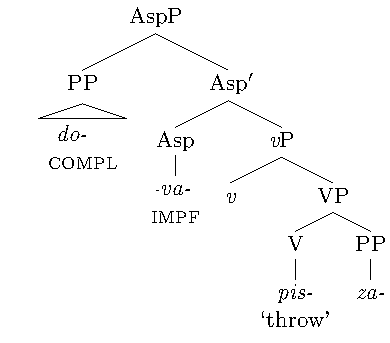
\includegraphics{dozapisyvat-Sven.pdf}
\begin{forest}
[AspP
 [PP [\Prefix{do-}\\\COMPL,align=center,roof]]
 [Asp'
   [Asp [-\textit{yva}-\\\IPF,align=center] ]
        [\textit{v}P
          [\textit{v}]
          [VP
            [V [\textit{pis}-\\`throw',align=center]]
            [PP [\textit{za}-]]
          ]
        ]
 ]
]
\end{forest}
\end{figure}

\begin{figure}
\caption{Tree for \textit{dozapisyvat'} `to (be) finish(ing) writing' according to the proposal in \citet{Tatevosov:07}\label{tree:tat}}
% % 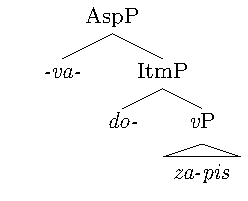
\includegraphics{dozapisyvat-Tat07.pdf}
\begin{forest}
[AspP
 [-\textit{yva}-]
 [ItmP
   [\textit{do}-] [\textit{v}P [\textit{za-pis},roof]]
 ]
]
\end{forest}
\end{figure}

% states, that when a \isi{lexical prefix} and a \isi{superlexical} co-occur with the \isi{secondary imperfective} suffix, the resulting word behaves like a perfective, i.e., the scoping is similar to what was proposed by \citet[ex.~(70)]{Svenonius:03}, corresponding to the rule (e) in the schema above.\\
Contrary to both \citet{Svenonius:04b} and \citet{Ramchand:04}, \citet{Tatevosov:07} arrives at a different aspectual classification of the same verb. This is because according to \citet{Tatevosov:07}, \textit{do}- occupies a special projection for \isi{intermediate prefixes} so that the resulting \isi{syntactic structure} is as on \figref{tree:tat}. As we see, the \isi{imperfective suffix} is in the highest position and the aspect of the whole verb must be imperfective. 

As is shown by the examples above, approaches such as \citet{Svenonius:04b}, \citet{Ramchand:04}, \citet{Romanova:06}, and \citet{Tatevosov:07} predict exactly one \isi{syntactic structure} for the verb \textit{dozapisyvat'}, as well as for any other verb. This holds even for the most detailed account by \cite{Tatevosov:09}. Here the existence of an exceptional group of \isi{superlexical} prefix uses is postulated. This group is the group of \isi{selectionally limited prefixes} and includes \isi{delimitative} \Prefix{po-}, \isi{cumulative} \Prefix{na-}, \isi{distributional} \Prefix{pere-} and \isi{inchoative} \Prefix{za-}. These prefixes, according to \citet{Tatevosov:09}, can take a position ``above'' or ``below'' the \isi{imperfective suffix} as long as the source verb is imperfective (which is not allowed in other approaches). However, this fact does not affect the overall prediction that there is a unique \isi{syntactic structure} assigned to each given complex verb (with fixed interpretation) due to the selectional restriction.

This conclusion is not immediately obvious, so let us consider an example. Verbs that follow the Scheme~\ref{form:do} contain the \isi{imperfective suffix} and two prefixes, the outermost of which, \Prefix{do-}, is, according to \citet{Tatevosov:09}, selectionally limited (can only be attached to a formally imperfective verb). As \isi{selectionally limited prefixes} can appear either higher or lower than the \isi{imperfective suffix}, there seems to be a potential for the \isi{structural ambiguity}. Examples of such verbs are \textit{zazapisyvat'} `to start writing down/recording' and  \textit{nazapisyvat'} `to write down/record a lot'. It turns out that for such verbs there is a unique order of affix attachment possible, as the second prefix cannot be attached earlier than the \isi{imperfective suffix} because of the selectional restriction.

One exception to the rule ``one verb -- one structure'' is a modification of \citet{Tatevosov:09} sketched in \citet{Tatevosov:13} that seems to implicitly react to problematic examples first mentioned in \citet{Zinova:12}. \citet{Tatevosov:13} proposes that the \isi{completive} prefix \Prefix{do-} (\isi{for a certain group of Russian speakers}) does not have any restrictions on its attachment. If, however, such modification is adopted without further restrictions, the predicted class of \isi{biaspectual verbs} ends up beeing too large. This problem may be solvable, but, as no solution is offered by the author, I will not discuss this proposal further.

%
%Let us suppose that we modify the syntactically based approaches in such a way that they would allow syntactic ambiguity. Even giving them the benefit of doubt that their analyses can be extended, this still leads to the following problem. Let us consider two verbs following the pattern in (1): dozapisyvat’ ‘to finish writing down’ and dovyshivat’ ‘to finish embroidering.’ These verbs have exactly the same affixes involved: a \isi{lexical prefix}, a \isi{superlexical} prefix \isi{do-} with \isi{completive} meaning and the \isi{imperfective suffix}. However, these verbs exhibit a clear difference in their usage: dozapisyvat’ is primary imperfective (about one half of the speakers accept it as being both perfective and imperfective, all accept it as an imperfective verb) while dovyshivat’ is primary perfective (all naïve native speakers that were questioned accept it as a perfective verb and most do not accept it as an imperfective verb). Such behaviour is completely unexpected under any syntactic theory, as from the syntactic point of view these verbs are identical and must exhibit the same properties.\\
In sum, the notion of a structural position is helpful in motivating at least certain facts about the formation of \isi{complex verbs} (as shown by example \ref{ex:pred}). For this reason syntactic approaches were a necessary step in the process of understanding Russian \isi{prefixation} system. However, the problematic part of these approaches is that, as I have shown, they exclude the existence of \isi{biaspectual affixed verbs}. The reason for this is that the postulated structural assumptions force a given complex verb to be assigned exactly one structure. This structure, in turn, determines the aspect of the verb independently of any other factors. An attempt to overcome the ``one verb -- one structure'' restriction without subdividing the class of \isi{superlexical} prefixes even further  \citep{Tatevosov:13} leads to massive overgeneration. The problem, in my view, lies in the assumption of a strict distinction between lexical and \isi{superlexical} prefixes. In Chapter~\ref{Chapter4} we will discuss in detail properties that are assigned to each class and I will show that there is no evidence for a strict classification, as each property is true of a different set of prefix usages.

\subsection{Diagnostics for aspectual classes}\label{sec:tests:old}
Several \isi{tests are commonly used} to establish the aspect of a given verb in Russian. Surprisingly, all of them are designed to exclude the possibility that it is perfective. Hence, they focus on the negative formal properties of \isi{perfective verbs}. The following test set is provided by \citet{Schoorlemmer:95}: 
\ex.\label{tests} \a.[(i)] \label{sttest1} \isi{perfective verbs} \textit{do not} get an ``ongoing'' interpretation in nonpast tense; 
\b.[(ii)] \label{sttest2} \isi{perfective verbs} \textit{cannot} be used as complements of \isi{phasal verbs} (e.g., \textit{na\v{c}at'} `to begin'); 
\b.[(iii)] \label{sttest3} \isi{perfective verbs} \textit{cannot} form \isi{present participles}.

\subsubsection{Non-past tense reading test}
This test is concerned with the interpretation possibilities for verbs with present tense morphology. Perfective verbs, as illustrated by \ref{ex:fut:2}, cannot receive present \isi{progressive interpretation}, as opposed to imperfectives \ref{ex:fut:1}.

\ex.\label{ex:fut}\ag.\label{ex:fut:1}Vasja pi\v{s}et\textsuperscript{\IPF} pis'mo.\\
Vasja write.\glb{pres.3.sg} letter\\
`Vasja is writing a letter.'
\bg.\label{ex:fut:2}Vasja napi\v{s}et\textsuperscript{\PF} pis'mo.\\
Vasja na.write.\glb{pres.3.sg} letter\\
`Vasja will write a letter.'
 
\subsubsection{Phase verbs}
There is a group of verbs that can take either nominals or infinitives as their complements. These verbs are called \textit{phase verbs}. In \cite{Borik:02} the following list of such verbs is provided:
\begin{itemize}[noitemsep]
\item \textit{na\v{c}inat'} `begin'
\item \textit{prodol\v{z}at'} `continue'
\item \textit{zakan\v{c}ivat'} `finish'
\item \textit{kon\v{c}at'} `finish'
\item \textit{perestavat'} `stop'
\end{itemize}
The test uses the fact that only \isi{imperfective verbs} can be complements of the phrase verbs, as illustrated by \ref{ex:phrase}.

\ex.\label{ex:phrase}\ag.Vasja na\v{c}al pisat'\textsuperscript{\IPF}/*napisat'\textsuperscript{\PF} pis'mo.\\
Vasja began write.\glb{inf} letter\\
Vasja began writing a letter
\bg.Ma\v{s}a zakon\v{c}ila \v{c}itat'\textsuperscript{\IPF}/*pro\v{c}itat'\textsuperscript{\PF} knigu.\\
Masha finished read.\glb{inf} book\\
Masha finished reading the book

\subsubsection{Present participles}
\textcite{Borik:02} offers a \isi{test for perfectivity} based on the fact that \isi{present participles} can only be derived from \isi{imperfective verbs}. There are four kinds of participles in Russian, as shown on Table~\ref{table:part}. They are characterised by two properties: tense (present or \isi{past}) and voice (active or passive).
\begin{table}
\caption{Verbal participles in Russian}\label{table:part}
\begin{tabularx}{\textwidth}{lQQ}
\lsptoprule
 & active & passive\\\midrule
  present &  \v{c}it-a-ju\v{s}\v{c}-ij `reading' & \v{c}it-a-em-yj `being read' \\
  \isi{past} & \v{c}it-a-v\v{s}-ij `reading' (\isi{past}); pro-\v{c}it-a-v\v{s}-ij `having read' & \v{c}it-a-nn-yj `being read' (\isi{past}); pro-\v{c}it-a-nn-yj `having been read'\\
\lspbottomrule
\end{tabularx}
\end{table}

Present active participles  (PAPs) are more common than present passive participles, so they are more convenient to use for aspect testing. As they denote ongoing progressive events, they can only be formed from imperfective stems. Examples~\ref{ex:part1} and \ref{ex:part2} illustrate how the test can be applied: \ref{ex:part11} shows the formation of a \isi{present active participle} of the imperfective verb \textit{\v{c}itat'} `to read'. Example \ref{ex:part12} shows that in case of the perfective verb \textit{pro\v{c}itat'} `to read through' such formation is not possible.\footnote{There are, however, some participles that are formed from \isi{perfective verbs} and are widely accepted (although not included in the literary norm), such as \textit{zainteresuju\v{s}\v{c}ij} `that will interest you' as evidenced by \ref{ex:PFP}.
\exg.\label{ex:PFP}vy mo\v{z}ete samostojatel'no zapisat'sja i pose\v{s}\v{c}at' zainteresuju\v{s}\v{c}ij vas kurs\\
you.\glb{nom} can {on your own} za.write.\glb{inf.refl} and visit.\glb{inf} za.interest.\glb{pap.sg.m} you.\glb{acc} course.\glb{acc}\\
\trans `you can on your own inscribe and visit a course that you will find interesting'\\\hbox{} \hfill \hbox{\url{https://www.nstu.ru/entrance/answers/view?num=39005}, accessed on 21.07.21}

} Example \ref{ex:part2} illustrates the same distribution for the verbs \textit{pisat'}\textsuperscript{\IPF} `to write' and \textit{napisat'}\textsuperscript{\PF} `to write down'.

\ex.\label{ex:part1}\ag.\label{ex:part11}\v{c}it-a-ju\v{s}\v{c}-ij\\
read\textsuperscript{\IPF}.\glb{PAP.sg.m}\\
reading
\bg.\label{ex:part12}*pro-\v{c}it-a-ju\v{s}\v{c}-ij\\
pro.read\textsuperscript{\PF}.\glb{PAP.sg.m}\\

\ex.\label{ex:part2}\ag.\label{ex:part21}pi\v{s}-u\v{s}\v{c}-ij\\
write\textsuperscript{\IPF}.\glb{PAP.sg.m}\\
writing
\bg.\label{ex:part22}*na-pi\v{s}-u\v{s}\v{c}-ij\\
write\textsuperscript{\PF}.\glb{PAP.sg.m}\\
\z.


\subsection{A positive test for perfectivity}\label{sec:tests:new}\largerpage
As we have just seen, \isi{perfective verbs} are commonly distinguished from imperfectives by tests that specify the properties that perfectives fail to have. While these tests delimit \isi{perfective verbs}, they cannot distinguish between imperfective and \isi{biaspectual verbs}. Based on the previous aspect research, there seem to be two more possible candidate \isi{tests for perfectivity}: one relies on \isi{past passive participle} formation and the other makes use of the properties of the \isi{narrative sequence}. %We will ultimately show that neither of them works. 

According to the first potential test, \isi{past} passive participles (PPPs) can only be formed from \isi{perfective verbs}. For example, in the pairs of verbs shown in \ref{pair} while the perfective member sanctions the derivation of a PPP \ref{ppp2}, the imperfective one is not supposed to do so \ref{ppp1}.
\exg.\label{pair}{gruzit'\textsuperscript{\IPF}} {$\rightarrow$} zagruzit'\textsuperscript{\PF}\\
{`to load'} {} {`to load completely'}\\

\ex.\ag.\label{ppp1}gruzit'\textsuperscript{\IPF} $\nrightarrow$ *gru\v{z}ennyj\\
{`to load'} {~} {~}\\
\bg.\label{ppp2}zagruzit'\textsuperscript{\PF} {$\rightarrow$} zagru\v{z}ennyj\\
{`to load'} {~} {`loaded'}\\

However, matters are not as simple as that. As has been pointed out by \citet{Schoorlemmer:95}, this test is applicable only to transitive and \isi{aspectually paired verbs}. Specifically, according to Schoorlemmer, no \isi{perfective verbs} with \isi{superlexical} prefixes form \isi{aspectual pairs}, which makes the test of little help for our purposes. Second, \citet{Romanova:06} provides a number of counterexamples of \isi{past} passive participles derived from \isi{imperfective verbs}, among others \ref{pppcontr}.
\exg.\label{pppcontr}kolonna avtoma\v{s}in, gru\v{z}ennyx buma\v{z}nymi paketami \\
column.\glb{nom} car.\glb{pl.gen} loaded.\glb{part.pass.pst.pl.gen} paper.\glb{pl.inst} bags.\glb{inst}\\
\trans `a string of cars, loaded with paper bags'\hfill\hbox{= ex. (9c) in \citet[5]{Romanova:06}}

As a consequence, the PPP formation test appears to be neither reliable nor general enough.\largerpage

The second possible positive test is connected to the phenomenon of \isi{aspectual pairs} and to the contribution of the verbal aspect to the \isi{narrative sequence}. Both are evoked in connection with what is referred to as the \textit{\isi{Maslov criterion},} which first appears in the following formulation \citep[][76--77]{Maslov:04}: 
\begin{quote}
``Pri perevode povestvovanija iz ploskosti pro\v{s}ed\v{s}ego vremeni v ploskost' istori\v{c}eskogo nastoja\v{s}\v{c}ego vse glagoly kak SV, tak i NSV, okazyvajutsja uravnennymi v formax nastoja\v{s}\v{c}ego vremeni NSV.'' [When the narrative is transformed from the \isi{past} into the \isi{historical present}, all the verbs, both perfective and imperfective, result in present tense forms of \isi{imperfective verbs}.] 
\end{quote}
However, the specific reference to Maslov's work is typically not given when the criterion is applied. Here is a citation from \citet[1]{Mikaelian:07}, who provide one of the clearest formulations:

\begin{quote}
``A perfective and an imperfective verb can be considered an \isi{aspectual pair} if and only if the imperfective verb can be substituted for the perfective verb in situations (such as descriptions of reiterated events or narration in \isi{historical present}) where the latter is not allowed.'' 
\end{quote}

\citet{Mikaelian:07} illustrate the above with the following contrast: 
\ex.\label{maslov}\ag.\label{maslov1}Pri\v{s}el\textsuperscript{\PF}, uvidel\textsuperscript{\PF}, pobedil.\textsuperscript{\PF}\\
come.\glb{\isi{past}.sg.m}, see.\glb{pst.sg.m}, conquer\glb{.pst.sg.m}\\
\trans `I came, I saw, I conquered.'
\bg.\label{maslov2}Prixo\v{z}u\textsuperscript{\IPF}, vi\v{z}u\textsuperscript{\IPF}, pobe\v{z}daju.\textsuperscript{\IPF}\\
come.\glb{pres.1.s}g, see.\glb{pres.1.sg}, conquer.\glb{pres.1.sg}\\
\trans `I come, I see, I conquer.'

The sentence \ref{maslov1} describes a sequence of events in the \isi{past}, suggesting that each event was completed before the next started. Now, if the speaker wants to represent the same state of affairs in the \isi{historical present} or as a \isi{habitual situation} (their ``reiterated event''), due to independently motivated constraints on the Russian aspectual system, only the corresponding\footnote{``Corresponding'' is understood as the imperfective verb that constitutes the \isi{aspectual pair} in the traditional sense with the original perfective verb.} \isi{imperfective verbs} can be used, as in \ref{maslov2}.

It is plausible to approach \isi{biaspectual verbs} by considering them as a kind of a covert \isi{aspectual pair} and then apply the \isi{Maslov criterion} in order to find them. One of the verbs that are often cited as a paradigm example of a native biaspectual verb is \emph{kaznit'} `to execute'. If the verbs in \ref{pairpref} and \ref{pairsuf} can be thought of as constituting an \isi{aspectual pair}, then the verb \textit{kaznit'} `to execute' in two different aspects in \ref{pairbi} might be thought of along the same lines, but of course in \ref{pairbi} the alleged members of the \isi{aspectual pair} just happen to be not phonologically differentiated.\largerpage

\ex.\ag.\label{pairpref}{pisat'\textsuperscript{\IPF}} {$\rightarrow$} {napisat'\textsuperscript{\PF}}\\
{`to write'} {} {`to write'}\\
\bg.\label{pairsuf}{zapisat'\textsuperscript{\IPF}} {$\rightarrow$} {zapisyvat'\textsuperscript{\PF}}\\
{`to write down'} {} {`to write/be writig down'}\\
\bg.\label{pairbi}{kaznit'\textsuperscript{\IPF}} {$\rightarrow$} {kaznit'\textsuperscript{\PF}}\\
{`to execute'} {} {`to execute'}\\

When one applies the test, illustrated by \ref{maslov}, to \textit{kaznit'} `to execute', one can see that it can be used in the \isi{narrative sequence}  \ref{maslovkaznit1}. This seems to suggest that it behaves like a perfective verb. The same verb can be used in the \isi{historical present} or the \isi{habitual situation} \isi{context}, strongly suggesting that in \ref{maslovkaznit2} \textit{kaznit'} `to execute' behaves like an imperfective verb.
\ex.\label{maslovkaznit}\ag.\label{maslovkaznit1}Pri\v{s}el\textsuperscript{\PF}, uvidel\textsuperscript{\PF}, pobedil\textsuperscript{\PF}, kaznil\textsuperscript{\PF} vragov.\\
come.\glb{pst.sg.m}, see.\glb{pst.sg.m}, conquer.\glb{pst.sg.m}, execute.\glb{pst.sg.m} enemies\\
\trans `I came, I saw, I conquered, I executed the enemies.'
\bg.\label{maslovkaznit2}Prixo\v{z}u\textsuperscript{\IPF}, vi\v{z}u\textsuperscript{\IPF}, pobe\v{z}daju$^{I{\PF}}$, kaznju$^{IPF}$ vragov.\\
come.\glb{pres.1.sg}, see.\glb{pres.1.sg}, conquer.\glb{pres.1.sg}, execute.\glb{pres.1.sg} enemies\\
\trans `I come, I see, I conquer, I execute the enemies.'

This would seem to be in compliance with the \isi{Maslov criterion}, as formulated by \citet{Mikaelian:07}. Therefore, \ref{maslovkaznit} seems to indicate that \isi{biaspectual verbs} like \textit{kaznit'} `to execute' could be treated as covert \isi{aspectual pairs}: in \ref{maslovkaznit1} the verb is perfective, while in \ref{maslovkaznit2} it is imperfective.

However, in the same contexts (\isi{narrative sequence} and \isi{historical present}\slash \isi{habitual situation}) it is also possible to use \isi{imperfective verbs} like \textit{dumat'} `to think', as illustrated by the examples \ref{maslovdumat1} and \ref{maslovdumat2}.
\ex.\label{maslovdumat}\ag.\label{maslovdumat1}Pri\v{s}el\textsuperscript{\PF}, uvidel\textsuperscript{\PF}, pobedil\textsuperscript{\PF}, dumal\textsuperscript{\IPF} o budu\v{s}\v{c}em.\\
come.\glb{pst.sg.m}, see.\glb{pst.sg.m}, conquer.\glb{pst.sg.m}, think.\glb{pst.sg.m} about future\\
\trans `I came, I saw, I conquered, I thought about the future.'
\bg.\label{maslovdumat2}Prixo\v{z}u\textsuperscript{\IPF}, vi\v{z}u\textsuperscript{\IPF}, pobe\v{z}daju\textsuperscript{\IPF}, dumaju\textsuperscript{\IPF} o budu\v{s}\v{c}em.\\
come.\glb{pres.1.sg}, see.\glb{pres.1.sg}, conquer.\glb{pres.1.sg}, execute.\glb{pres.1.sg} about future\\
\trans `I come, I see, I conquer, I think about the future.'

This shows that such contexts cannot be used as diagnostics for perfectivity and imperfectivity. The \isi{Maslov criterion} requires a perfective verb as an input condition, so it is also negative for perfectivity. It allows to delimit the class of exclusively \isi{perfective verbs}, but does not allow to distinguish between biaspectual and \isi{imperfective verbs}. In \ref{maslovkaznit} the same verb is used in both sentences due to its \isi{biaspectual nature}. At the same time the possibility of using the same verb in both sentences in \ref{maslovdumat} is explained by the imperfective aspect of \textit{dumal} `thought' in the first sentence. Moreover, there are other conceptual problems related to the application of the \isi{Maslov criterion}.\footnote{\citet[2]{Mikaelian:07} write that ``rather than a tool for establishing \isi{aspectual pairs}, the \isi{Maslov criterion} should be taken as a definition and raison d'\^etre of the aspectual correlation.''}

The crucial point to be made here is that no reliable positive \isi{test for perfectivity} has been proposed so far.\footnote{A new proposal to overcome this problem has been recently offered by \citet{Piperski:biasp}. The author suggests using gerund forms to identify the aspect of the verb, as each verb that is not biaspectual has exactly one gerund form, ``which denotes simultaneity for \isi{imperfective verbs} and precedence for \isi{perfective verbs}'' (p. 5). Moreover, the imperfective  and perfective gerunds are formally distinguishable, as the former ~~one~~ is marked by the \textit{-a/-ja} suffix, whereas the latter uses the \textit{-v/-v\v{s}i} suffix. It turns out that \isi{biaspectual verbs} can form the gerund in both ways, which allows us to identify them. The only drawback of this test is that, as the author notes himself, it does not work for all verbs, but only for those that contain the suffix \is{suffix!-ova-}\textit{-ova-} or the suffix \textit{-a-} (and does not work with verbs whose stems end in \textit{-e-} and \textit{-i-}).} Figure~\ref{circles} schematically represents the aspectual classes of Russian verbs. The standard tests listed in \ref{tests} are negative for perfectivity. They merely exclude the possibility that a given verb form is a member of Set 1. To separate the subset of \isi{biaspectual verbs} (Set 3) from true \isi{imperfective verbs} (Set 2), we need a positive \isi{test for perfectivity} (Set 1). In combination with the standard tests, we can then identify the class of the \isi{biaspectual verbs}.\largerpage

\begin{figure}
% % \includegraphics[scale=1]{EulerCircles}\\
\caption{\label{circles}Aspectual classes}
\begin{tikzpicture}[every fit/.style={ellipse,draw,inner xsep=-10pt,inner ysep=\baselineskip}]
\node at (0,0) (perfective) {(1) perfective};
\node [right=1.5cm of perfective] (biaspectual) {(3) biaspectual};
\node [right=1.5cm of biaspectual] (imperfective) {(2) imperfective};
\node [fit = (perfective) (biaspectual)] {};
\node [fit = (imperfective) (biaspectual)] {};
\end{tikzpicture}
\end{figure}

The new positive \isi{test for perfectivity} proposed in \citet{ZinovaFilip:13} capitalises on the notion of the \textit{Narration relation}, defined by \citet{Lascarides:93} as follows:

\begin{quote}
\textit{Narration($\alpha,\beta$)}: The event described in $\beta$ is a consequence of (but not strictly speaking caused by) the event described in $\alpha$. If \textit{Narration ($\alpha,\beta$)} holds, and $\alpha$ and $\beta$ describe eventualities \textit{e$_1$} and \textit{e$_2$}, respectively, then \textit{e$_1$} occurs before \textit{e$_2$}.
\end{quote}

The \textit{Narration} relation can be illustrated by \ref{textnar}: 
\ex.\label{textnar} Max woke up. He opened the window. 

In English, it is natural to use \isi{telic verb} phrases in non-progressive tense in the \textit{Narration} relation. A parallel Russian example \ref{narrus} contains two \isi{perfective verbs}. It is well-known  in the literature on aspect and \isi{discourse structure} that the main line of a narrative is constituted by sequences of perfective verb forms which move narrative time forward \citep[for Russian, see in particular][]{Paducheva:96, Paducheva:04}.

\exg.\label{narrus}Maksim prosnulsja\textsuperscript{\PF}. On otkryl\textsuperscript{\PF} okno.\\
Maksim woke.up.\glb{pst.sg.m}.refl he open.\glb{pst.sg.m} window.\glb{sg.acc}\\
\trans `Maksim woke up. He opened the window.'

The property the test relies on is that if the Narration relation holds and the second verb is perfective, the aspect of the first verb must be perfective as well. Example \ref{narrusbad} demonstrates that the combination of an imperfective and a perfective verb is uninterpretable. Under the most normal assumptions about how situations in the world take place, people do not open the windows while sleeping, nor is the event of opening a window normally interpreted as result or a continuation of the waking up event. Given that, the only possible relation between the two events (waking up and opening the window) is \textit{Narration}.
\exg.\label{narrusbad}$^{??}$Maksim prosypalsja\textsuperscript{\IPF}. On otkryl\textsuperscript{\PF} okno.\\
\hspaceThis{$^{??}$}Maksim woke.up.imp.\glb{pst.sg.m}.refl he open.\glb{pst.sg.m} window.\glb{sg.acc}\\
\trans\hspaceThis{$^{??}$}`Maksim was waking up. He opened the window.'\footnote{The English translation of this discourse seems to be much better than the Russian original. This effect is probably due to the different range of possible interpretations of the verbs \textit{prosypat'sja} `to wake up' and \textit{to wake up}. The Russian verb \textit{prosypat'sja} `to wake up' can only refer to the period before getting out of bed.}

\begin{table}
\caption{\label{table}Verbal aspect and the \textit{Narration} relation}
\begin{tabular}{llc}
\lsptoprule
\multicolumn{2}{c}{Verbal combination}& Acceptability judgment\\\midrule
perfective verb & \textit{i} `and' perfective verb~ & ok\hphantom{\textsuperscript{\textit{a}}}\\
imperfective verb & \textit{i} `and' perfective verb~ & ??\footnote{I use this sign to indicate a problem on the discourse level.}\\
biaspectual verb & \textit{i} `and' perfective verb~ & ok\hphantom{\textsuperscript{\textit{a}}}\\
\lspbottomrule
\end{tabular}
\end{table}

The idea of the test is summarised in Table~\ref{table}. \citet{ZinovaFilip:13} propose to use as test contexts sentences like \ref{test1} and \ref{test2}. The task is to enforce the Narration relation  between the two clauses (see more details below). In this case if the verb in the second clause is perfective, the first verb must be perfective as well. Example~\ref{test1} is in the non-\isi{past}, whereas \ref{test2} -- in the \isi{past} tense. This shows that tense is not relevant for the purpose of the test. Note that this is not to deny that the Narration relation may also hold in sequences with \isi{imperfective verbs} only, as in \ref{ex:nar:imp}.
\ex.\label{test1}\ag.\label{test11}Ja s''em\textsuperscript{\PF} zavtrak i pojdu\textsuperscript{\PF} na rabotu.\\
I s.eat.\glb{pres.1.sg} breakfast and po.go.\glb{pres.1.sg} on work\\
\trans `I will finish my breakfast and go to work.'
\bg.\label{test12}$^{??}$Ja em\textsuperscript{\IPF} zavtrak i pojdu\textsuperscript{\PF} na rabotu.\\ 
\hspaceThis{$^{??}$}I eat\glb{.pres.1.sg} breakfast and po.go.\glb{pres.1.sg} to work\\

\ex.\label{test2}\ag.\label{test21}Ja s''el\textsuperscript{\PF} zavtrak i po\v{s}el\textsuperscript{\PF} na rabotu.\\
I s.eat.\glb{pst.sg.m} breakfast and po.go.\glb{pst.sg.m} on work\\
\trans `I finished my breakfast and went to work.'
\bg.\label{test22}$^{??}$Ja el\textsuperscript{\IPF} zavtrak i po\v{s}el\textsuperscript{\PF} na rabotu.\\
\hspaceThis{$^{??}$}I eat.\glb{pst.sg.m} breakfast and po.go.\glb{pst.sg.m} to work\\

\exg.\label{ex:nar:imp}U\v{z}e 8:00. Ja em\textsuperscript{\IPF} zavtrak i idu\textsuperscript{\IPF} na rabotu.\\
already 8:00. I eat.\glb{pres.1.sg} breakfast and go.\glb{pres.1.sg} to work\\
\trans `It is already 8:00. I eat breakfast and go to work.'

Examples \ref{test11} and \ref{test21} illustrate the first line of the table, \ref{test12} and \ref{test22} -- the second line of the table. \ref{test12} and \ref{test22} are not interpretable, because neither the Narration relation nor any other \isi{coordinating relation}, e.g., a \isi{Background} relation, can be construed. 

Examples \ref{biasp} illustrate the third line of the table above, which is crucial in case of \isi{biaspectual verbs}. In a given \isi{context}, \textit{kaznit'} `to execute' can behave either as a perfective or as an imperfective verb. Given that in the test \isi{context} \isi{imperfective verbs} are odd, \isi{biaspectual verbs} pattern together with \isi{perfective verbs}. Thus, the proposed test \isi{context} allows us to distinguish between biaspectual and \isi{imperfective verbs}. 
\ex.\label{biasp}\ag.Pala\v{c} kaznit prestupnika i pojd\"et\textsuperscript{\PF} domoj.\\
hangman execute.\glb{pres.3.sg} criminal and po.go.\glb{pres.3.sg} home\\
`The hangman will execute the criminal and will go home.'
\bg.Pala\v{c} kaznil prestupnika i po\v{s}el\textsuperscript{\PF} domoj.\\
hangman execute.\glb{pst.sg.m} criminal and po.go.\glb{pst.sg.m} home\\
`The hangman executed the criminal and went home.'

Now that the basic workings of the test are explained, let me address the precise conditions under which it works as a positive \isi{test for perfectivity}. To enforce the \textit{Narration} relation, the following conditions are required to be met:
\begin{enumerate}
\item The main lexical verb in the second clause must have a \isi{temporal extent}.
\item The event denoted by the main lexical verb in the second clause must not be caused or considered a continuation of the event denoted by the main lexical verb in the first clause.
\item The clauses must be conjoined using plain \isi{conjunction} \textit{i} `and' without any temporal or modal (epistemic) adverbial.
\end{enumerate}
The conditions above reveal the workings of the test. When the clauses headed by two verbs, where the second one is perfective, are conjoined with \textit{i} `and' (condition 3), several coordinating \isi{discourse relations} can be established between them. Conditions 1 and 2 ensure that such coordinating relations as \isi{Background} or \isi{Cause} are excluded. After this the only possible relation between the two clauses is Narration. If the Narration relation  cannot be established, the discourse is infelicitous, as in \ref{test12} and \ref{test22}.

The reason for the first condition is that verbs denoting \isi{punctual events} could be construed as describing events that are temporally located within the time span of the first event. In such a case, it is not the Narration (but the \isi{Background}) relation that holds between the two clauses, and thus the rule expressed in the last line of the table above (Table~\ref{table}) is not applicable, as illustrated by \ref{test5}. This condition is relevant if the test is applied in the \isi{past} tense.
\exg.\label{test5}Ona igrala\textsuperscript{\IPF} v futbol i slomala\textsuperscript{\PF} nogu.\\
she play.\glb{pst.sg.f} in football and break.\glb{pst.sg.f} leg\\
\trans `While she was paying football, she broke her leg.'

\exg.\label{ex:cause}Ona xoro\v{s}o igrala\textsuperscript{\IPF} i zarabotala\textsuperscript{\PF} nagradu.\\
she well play.\glb{pst.sg.f} and za.work.\glb{pst.sg.f} reward\\
\trans `She was playing well and earned a reward.'

Examples like \ref{ex:cause} show the importance of the second condition: if the events denoted by the two main verbs are connected, the \isi{discourse relation} is not one of Narration. According to \citet{Txurruka:03}, the natural language \isi{conjunction} `and' marks a \isi{coordinating relation}, which means is a relation of Narration, \isi{Background}, Result, Continuation, Parallel or Contrast \citep{Asher:05}. To ensure a proper application of the test, one has to establish a \isi{context} where the \isi{Narration relation} is the only possible one between the two events. 

On the basis of the observation by \citet{Txurruka:03} that Narration is marked by \textit{then}, I propose to use the \isi{substitution} of \textit{potom} `then' instead of \textit{i} `and' to check whether it is in fact Narration that connects the two coordinated clauses. If it is, then the meaning of the two sentences is (nearly) identical (compare \ref{test1} with \ref{breakfast:potom}). If it is not, the meaning changes significantly after such a \isi{substitution}. To see this, compare \ref{test5} with \ref{football:potom} and \ref{ex:cause} with \ref{ex:cause:potom}: the sentences in \ref{football:potom} and \ref{ex:cause:potom} suggest that the second event is not caused or explained by the first one. These examples also illustrate why \textit{potom} `then' cannot be used for the purposes of the test directly: it establishes the \isi{Narration relation} even in case of the different aspects of the main verbs in the two clauses.

\ex.\ag.\label{breakfast:potom}Ja s''em\textsuperscript{\PF} zavtrak, potom pojdu\textsuperscript{\PF} na rabotu.\\
I s.eat.\glb{pres.1.sg} breakfast then po.go.\glb{pres.1.sg} on work\\
\trans `I will finish my breakfast, then I will go to work.'
\bg.\label{football:potom}Ona igrala\textsuperscript{\IPF} v futbol, potom slomala\textsuperscript{\PF} nogu.\\
she play.\glb{pst.sg.f} in football then break.\glb{pst.sg.f} leg\\
\trans `She was playing football, then she broke her leg.'
\bg.\label{ex:cause:potom}Ona xoro\v{s}o igrala\textsuperscript{\IPF}, potom zarabotala\textsuperscript{\PF} nagradu.\\
she well play.\glb{pst.sg.f} then za.work.\glb{pst.sg.f} reward\\
\trans `She was playing well, then she earned a reward.'

\ex.\label{test3}\ag.\label{test31}Ja em\textsuperscript{\IPF} zavtrak. Pojdu\textsuperscript{\PF} na rabotu.\\ 
I eat.\glb{pres.1.sg} breakfast po.go.\glb{pres.1.sg} to work\\
\trans `I'm eating breakfast. I will go to work.'
\bg.\label{test32}$^?$Ja em\textsuperscript{\IPF} zavtrak i potom pojdu\textsuperscript{\PF} na rabotu.\\ 
I eat.\glb{pres.1.sg} breakfast and afterwards po.go.\glb{pres.1.sg} to work\\
\trans `I'm eating breakfast and will go to work afterwards.'
\bg.\label{test33}$^?$Ja em\textsuperscript{\IPF} zavtrak i objazatel’no pojdu\textsuperscript{\PF} na rabotu.\\
I eat.\glb{pres.1.sg} breakfast and necessarily po.go.\glb{pres.1.sg} to work\\
\trans `I'm eating breakfast and I of course will go to work.'
\bg.\label{test34}Ja em\textsuperscript{\IPF} zavtrak. Potom pojdu\textsuperscript{\PF} na rabotu.\\
I eat.\glb{pres.1.sg} breakfast afterwards po.go.\glb{pres.1.sg} to work\\
\trans `I'm eating breakfast. I will go to work afterwards.'

Examples under \ref{test3} demonstrate why the second condition is important: a sequence of two sentences without a \isi{conjunction} or any explicit adverbial indicating their connection, as \ref{test31}, is acceptable in an appropriate \isi{context} (for example if someone is asked about his plans; a pause will be present between the two sentences in such a case). Sentences \ref{test32} and \ref{test33} are at least much better than \ref{test12} and \ref{test22}. The last sentence, \ref{test34}, is completely natural. In these cases the \isi{Narration relation} between the two clauses holds. In \ref{test32} and \ref{test34} it is explicit due to the presence of \textit{potom} `then' which, as mentioned above, is a marker of the \isi{Narration relation}. As the idea of the test is to exclude all the coordinating relations (the coordinating requirement is imposed by \textit{i} `and', so it must be present) except for Narration and see whether this relation can be established given that the verb in the second clause is perfective, it is important to not include an explicit marker of this relation in the test \isi{context} and, because that would force its application. Substituting  \textit{i} `and' with \textit{potom} `then' destroys the test \isi{context}, as the \isi{Narration relation} is enforced independently from the aspect of the verbs heading the clauses, as is evidenced by \ref{ex:potomcomma}.

\exg.\label{ex:potomcomma}Ja em\textsuperscript{\IPF} zavtrak, potom pojdu\textsuperscript{\PF} na rabotu.\\
I eat.\glb{pres.1.sg} breakfast afterwards po.go.\glb{pres.1.sg} to work\\
\trans `I'm eating breakfast, afterwards I will go to work.'

A similar situation is observed in the \isi{past} tense: \ref{test41} is perfectly acceptable in a \isi{context} in which the speaker remembers what he or she did on a given occasion, but only if there is a distinct pause between the two sentences; for \ref{test42}, there do not seem to be any clear judgments; and \ref{test43} is a plausible discourse.
\ex.\label{test4}\ag.\label{test41}Ja el\textsuperscript{\IPF} zavtrak. Po\v{s}el\textsuperscript{\PF} na rabotu.\\
I eat.\glb{pst.sg.m} breakfast. po.go.\glb{pst.sg.m} to work\\
\trans `I was eating breakfast. I went to work.'
\bg.\label{test42}$^?$Ja el\textsuperscript{\IPF} zavtrak i potom po\v{s}el\textsuperscript{\PF} na rabotu.\\
I eat.\glb{pst.sg.m} breakfast and afterwards po.go.\glb{pst.sg.m} to work\\
\trans `I was eating breakfast and went to work afterwards.'
\bg.\label{test43}Ja el\textsuperscript{\IPF} zavtrak. Potom po\v{s}el\textsuperscript{\PF} na rabotu.\\
I eat.\glb{pst.sg.m} breakfast. Afterwards po.go.\glb{pst.sg.m} to work\\
\trans `I was eating breakfast. I went to work afterwards.'

%\bg.\label{test52}Ona igrajet\textsuperscript{\IPF} v futbol i obyazatel'no slomajet\textsuperscript{\PF} nogu.\\
%She play.pres.3.sg in football and necesserely break.pres.3.sg leg\\
%She plays football and she will definitely break her leg once.
% The verb in the second clause is perfective and requires a time moment as an input. Such time moment, if not provided by an adverbial (condition 1), must be provided by the verb in the first clause, thus this verb must be perfective in order for the sentence to be felicitous.\\
Such examples should suffice to illustrate the basic intuition behind the test. The main idea of the test is the generalisation given by \citet{Jespersen:24} that, if the verb is imperfective, it does not trigger narrative progression (in our case it is the verb in the first clause). Theoretically speaking, the relevant background for the workings of the test is best outlined in \citet{Altshuler:12}.
His account of the discourse properties of the Russian imperfective  relies on a multi-coordinate approach to aspect. He proposes interpretations for the \textsc{narr} operator and for the aspectual operators and explains why only \isi{perfective verbs} are acceptable in \ref{ex:daniel:a} (ex. (73-a) in \citealt{Altshuler:12}), which is an example similar to our test \isi{context}.

\ex.\label{ex:daniel}\ag.\label{ex:daniel:a}Lev ko mne \textsuperscript{\JudgeOK}priexal\textsuperscript{\PF} / {{$^{\#}$}priez\v{z}al\textsuperscript{\IPF}}\\
Lev to me {\hspaceThis{\textsuperscript{\JudgeOK}}pri.arrive.\glb{pst.3.sg}} / {{\textcolor{white} {$^{\#}$}}pri.arrive.imp.\glb{pst.3.sg}}\\
\bg.i srazu po\v{s}el\textsuperscript{\PF} ku\v{s}at'.\\
and right.away po.go.\glb{pst.3.sg} eat\\
\trans `Lev arrived at my place and went to eat right away.'\\
\hbox{}\hfill\hbox{(73-a) in \citet{Altshuler:12}}


%A good way of testing whether a verb is perfective is to identify contexts that only allow perfectives and contexts in which perfectives are excluded. Such contexts are those where a narration relation is established between the verb in question and a clearly perfective/imperfective verb, as in \ref{context1} and \ref{context2}:\\
%
%\ex.\label{context1} \ag. \label{context1:1}*Ja dopisyvaju\textsuperscript{\IPF} text i pojdu\textsuperscript{\PF} domoj.\\
%I do.write.imp\glb{prs.1.sg} text and go.\glb{pres.1.sg} home\\
%\bg. \label{context2:1}Ja dopisyvaju\textsuperscript{\IPF} text i idu\textsuperscript{\IPF} domoj.\\
%I do.write.imp\glb{prs.1.sg} text and go.\glb{pres.1.sg} home\\
%I plan to finish writing the text and go home.
%
%\ex.\label{context2} \ag. \label{context1:2}Ja dozapisyvaju\textsuperscript{\PF} disk i pojdu\textsuperscript{\PF} domoj.\\
%I do.za.write.imp\glb{prs.1.sg} CD and go.\glb{pres.1.sg} home\\
%I will finish recording the CD and go home.
%\bg. \label{context2:2}Ja dozapisyvaju\textsuperscript{\IPF} disk i idu\textsuperscript{\IPF} domoj.\\
%I do.za.write.imp\glb{prs.1.sg} and go.\glb{pres.1.sg} home\\
%I plan to finish recording the CD and go home.

\subsection{Applying the test}\label{subsection:bi:apply}
Now let us apply the test to the verbs \textit{dopisyvat'} `to finish/be finishing writing' and \textit{dozapisyvat'} `to finish/be finishing recording'. According to the \isi{syntactic theories}, one aspect is always assigned to both verbs: either perfective \citep{Ramchand:04, Romanova:04, Svenonius:04b} or imperfective \citep{Tatevosov:07, Tatevosov:09}. However, as examples \ref{context1} and \ref{context2} show, these two verbs pattern differently with respect to the narration relation test. If the verb \textit{dopisyvat'} `to finish/be finishing writing' is inserted in the test \isi{context} in the non-\isi{past} tense, as in \ref{context1:1}, or in the \isi{past} tense, as in \ref{context1:2}, both sentences are infelicitous. When the same contexts are populated with the verb \textit{dozapisyvat'} `to finish/be finishing recording', both resulting sentences are non-problematic.
\ex.\label{context1} \ag. \label{context1:1}$^{??}$Ja dopisyvaju tekst i pojdu\textsuperscript{\PF} domoj.\\
{\hspaceThis{$^{??}$}}I do.write.imp.\glb{pres.1sg} text and po.go.\glb{pres.1.sg} home\\
\bg. \label{context2:1}Ja dozapisyvaju disk i pojdu\textsuperscript{\PF} domoj.\\
I do.za.write.imp.\glb{pres.1.sg} CD and po.go.\glb{pres.1.sg} home\\
\trans `I will finish recording the CD and go home.'

\ex.\label{context2} \ag. \label{context1:2}$^{??}$Ja dopisyval text i po\v{s}el\textsuperscript{\PF} domoj.\\
{\hspaceThis{$^{??}$}}I do.write.imp.\glb{pst.sg.m} tekst and po.go.\glb{pst.sg.m} home\\
\bg. \label{context2:2}Ja dozapisyval disk i po\v{s}el\textsuperscript{\PF} domoj.\\
I do.za.write.imp.\glb{pst.sg.m} CD and go.\glb{pst.sg.m} home\\
\trans `I finished recording the CD and went home.'

Examples \ref{context3:1} and \ref{context3:2} show that the same results as for \textit{dozapisyvat'} are obtained for other verbs formed following the same pattern for \isi{biaspectual verbs} \ref{form:do}. A good example is the verb \textit{dovy\v{s}ivat'} `to finish embroidering'. Notice that a verb with the same root but without the inner prefix \Prefix{vy-}, namely, \textit{do\v{s}ivat'}, `to finish/be finishing sewing', is not acceptable in the test \isi{context}, as shown by examples \ref{context3:3} and \ref{context3:4}.
\ex.\label{context3}\ag.\label{context3:3}$^{??}$Ja do\v{s}ivala platje i podarila\textsuperscript{\PF} ego sestre.\\
{\hspaceThis{$^{??}$}}I do.sew.imp.\glb{pst.sg.f} dress and po.present.\glb{pst.sg.f} it sister\\
$^{??}$`I was finishing sewing this dress and I presented it to my sister.'
\bg.\label{context3:1}Ja dovy\v{s}ivala kartinu i povesila\textsuperscript{\PF} e\"e.\\
I do.embroid.imp.\glb{pst.sg.f} picture and po.hang.\glb{pst.sg.f} it\\
\trans `I finished embroidering the picture and hung it (on the wall).'

\ex.\label{context31}\ag.\label{context3:4}$^{??}$Ja do\v{s}ivaju platje i podarju\textsuperscript{\PF} ego sestre.\\
{\hspaceThis{$^{??}$}}I do.sew.imp.\glb{pres.1.sg} dress and po.present.\glb{pres.1.sg} it sister\\
$^{??}$`I am finishing sewing this dress and I will present it to my sister.'
\bg.\label{context3:2}Ja dovy\v{s}ivala kartinu i povesila\textsuperscript{\PF} e\"e.\\
I do.embroid.imp.\glb{pst.sg.f} picture and po.hang.\glb{pst.sg.f} it\\
\trans `I finished embroidering the picture and hung it (on the wall).'

To summarise, I have shown that the verbs formed according to the pattern in \ref{form:do}, e.g., \textit{dozapisyvat'} `to finish/be finishing recording', behave like verbs that are traditionally considered biaspectual (e.g., \textit{kaznit'} `to execute') and are intractable in the syntactic approaches.

% Chapter 3

\section{Derivational graph}\label{section:graph}
\subsection{Introduction}
As we have seen in the previous section, the existing approaches to Russian \isi{prefixation} do not account for the full range of prefixed verbs data. Moreover, they often do not agree on the data or some important datapoint is missing or disregarded. This section is dedicated to the description of a structure that allows to reach an agreement on the \isi{prefixation} data and easily check the proposed generalisations, if a database, organised according to the definition provided here, is implemented. Material presented in this section is partially covered in \citet{ZinovaFilip:14b}.

In the last part of this section, \sectref{subsection:predict}, I will show how the aspect of the verb can be easily predicted if we have the \isi{derivational graph}, which is proposed here, at hand. In most cases such prediction is possible for a verb that is stored in the graph node exclusively on the basis of the information about the incoming edges. The cases where additional information (such as the aspect of the verb in the parent node) may be needed are discussed in Section~\ref{section:new:perfectivity}.

\subsection{Definitions}\label{section:chains:definition}
As we have seen in the previous chapter, some prefixed verbs can be derived in various ways. I propose to observe these possibilities carefully before excluding some of them that, at first glance, do not fit neatly into the common model of verbal \isi{prefixation}.

The notion of a ``\isi{derivational chain}'' used here is inspired by \citet{Karcevski:27} who proposed that ``[l]a valeur aspective d'un verbe d\'{e}pend de la place qu'il occupe dans la cha\^{i}ne de la d\'{e}rivation d\'{e}verbative'' [the aspectual value of a verb depends on its place in the chain of verbal derivation].

In the spirit of \citet{Karcevski:27}, the basic idea I pursue here is to infer the aspectual value (perfective or imperfective) of a given verb form from the \isi{derivational chain},\footnote{In \citet{ZinovaFilip:14b} we call it \textit{derivational history}.} rather than from the pure \isi{syntactic structure}, as it is done in contemporary syntactic analyses. I also want to put forward the idea that the \isi{derivational chain} does not have to be unique for a given verb. To formalise \citeauthor{Karcevski:27}'s (\citeyear{Karcevski:27}) suggestions about what constitutes a \isi{derivational chain}, I propose the following definition:\largerpage

\begin{definition}\label{def:history}
A verb V$_2$ is derived from a verb V$_1$ if and only if
\begin{enumerate}[noitemsep,nosep]
\item both V$_1$ and V$_2$ are attested in the language;
\item there is a \isi{morphological operation} (the extensive list of such operations is provided by \citealt{Shvedova:82}) such that it takes as an input the verb V$_1$ and provides as an output the verb V$_2$;
\item the meaning of V$_2$ can be monotonically (possibly not entirely \isi{compositionally}) derived from the meaning of V$_1$;
\item there is no other verb V$_3$ such that V$_3$ is derived from V$_1$ and V$_2$ is derived from V$_3$.
\end{enumerate}
\end{definition}

To illustrate the above definition of a \isi{derivational chain}, let us consider the verbs \textit{kupit'\textsuperscript{\PF}} and \textit{pokupat'\textsuperscript{\IPF}} `to buy'. There are three possible ways in which these verbs might be related, shown in \ref{chain:pokupat}.

\ex.\label{chain:pokupat}\ag.\label{chain:pokupat1}kup-i-t'\textsuperscript{\PF} $\rightarrow$ *po-kup-i-t' $\rightarrow$ po-kup-a-t'\textsuperscript{\IPF}\\	
{to buy} $\rightarrow$ $\cdots$ $\rightarrow$ {to buy/to be buying}\\
\bg.\label{chain:pokupat2}kup-i-t'\textsuperscript{\PF} $\rightarrow$ po-kup-a-t'\textsuperscript{\IPF}\\
{to buy} $\rightarrow$ {to buy/to be buying}\\
\bg.\label{chain:pokupat3}kup-i-t'\textsuperscript{\PF} *$\rightarrow$ kup-a-t'\textsuperscript{\IPF} *$\rightarrow$ po-kup-a-t'\textsuperscript{\IPF}\\
{to buy} *$\rightarrow$ {to bathe} *$\rightarrow$ {to buy/to be buying}\\

The derivation in \ref{chain:pokupat1} is excluded, because *\textit{pokupit'} does not exist (violation of the first condition). The derivation in \ref{chain:pokupat2} is fine with respect to the first and the second conditions, so what we have to check for is the third condition. I.e., that there is no other verb such that it is derived from \textit{kupit'}\textsuperscript{\PF} `to buy'.  A candidate verb, formally speaking, would be \textit{kupat'\textsuperscript{\IPF}}, but it has an unrelated meaning `to bathe someone' (violation of the third condition). This also means that \ref{chain:pokupat3} cannot be considered to constitute a \isi{derivational chain}.  

As we have just seen, the second chain, \ref{chain:pokupat2}, is a valid \isi{derivational chain}, according to the three conditions above. However, it includes simultaneous (happening at one derivational step) attachment of two morphemes (the prefix \Prefix{po-} and the suffix \textit{-a-}). In this work I will not deal with such derivations that include a simultaneous addition of two or more morphemes (including cases of \isi{prefixation} accompanied by the addition of the \isi{postfix}) or discontinuous morphemes. I will limit myself to providing a computational account of verbal derivational morphology only for derivations that include an attachment of a single morpheme at each derivational step.

To provide an extension to the example~\ref{chain:pokupat}, let us also consider the candidate \isi{derivational chains} for the verb \textit{napokupat'} `to buy a lot', presented in \ref{ex:napokupat}. The first candidate chain, \ref{ex:napokupat1}, demonstrates a violation of the third condition: there exists another verb (\textit{pokupat'} `to buy/be buying') such that it is derived from the verb \textit{kupit'} `to buy' and serves as a \isi{derivational base} for obtaining the verb \textit{napokupat'} `to buy a lot'. So, despite the fact that the verb \textit{napokupat'} `to buy a lot' is (indirectly) derived from the verb \textit{kupit'} `to buy', the derivation in \ref{ex:napokupat1} is not a valid \isi{derivational chain}. On the other hand, the chain in \ref{ex:napokupat2} is a \isi{derivational chain}, according to the definition above, although only the second step of it will receive an analysis in this work.\largerpage[-1]

\ex.\label{ex:napokupat}\ag.\label{ex:napokupat1}kup-i-t'\textsuperscript{\PF} $\rightarrow$ na-po-kup-a-t'\textsuperscript{\PF}\\	
{to buy} $\rightarrow$ {to buy a lot}\\
\bg.\label{ex:napokupat2}kup-i-t'\textsuperscript{\PF} $\rightarrow$ po-kup-a-t'\textsuperscript{\IPF} $\rightarrow$ na-po-kup-a-t'\textsuperscript{\PF}\\
{to buy} $\rightarrow$ {to buy/to be buying} $\rightarrow$ {to buy a lot}\\

There is also another way to represent and store the information carried by the \isi{derivational chains}, that is useful for computational purposes: a graph. Let us consider the following directed graph $D$: 
\begin{definition}\label{def:chain}
$D = (V,A)$, where V is a set of nodes labeled with verbs that are attested in the language and A is a set of ordered pairs of nodes. $\forall x,y \in V, (x,y) \in A$ iff  the verb that labels the node y can be derived from the verb that labels the node x (according to the \defref{def:history}).
\end{definition}

In what follows, I will call such graph $D$ a \textit{\isi{derivational graph}.} Paths in this graph are \isi{derivational chains} that are defined by \defref{def:history}. The number of connected components of the graph $D$ equals the number of verbal stems in the object language.

There exists a graph that is similar to the \isi{derivational graph} described here. It represents derivational relations between Russian verbs and is a part of the OSLIN database\footnote{\textit{Open source lexical information network}, available online at \url{}}, described in \cite{Borik:12}. The problem with this graph is that it is far from being complete, as the lexical items included are taken from dictionaries and, as we have already discussed, this covers a relatively small amount of prefixed verbs and almost none of the multiply prefixed verbs.

Let me also mention another database of Russian prefixed verbs\footnote{Available at \url{http://emptyprefixes.uit.no/}} provided by the CLEAR (Cognitive Linguistics: Empirical Approaches to Russian) group at the University of Troms{\o}. According to the description on the website, ``[t]his database contains information on 1,981 \isi{imperfective verbs} in Russian that form \isi{aspectual pairs} via \isi{prefixation}'', aggregating entries from \citet{MAS}, \citet{Ozegov:01},  and \citet{Cubberly:82} that were approved by a panel of native speakers. This database, however, was constructed for the purpose of exploring the ``empty'' prefixes and thus is not a full \isi{derivational graph} as it contains only verbs that form \isi{aspectual pairs} (imperfective and \isi{perfective verbs} with the same lexical meaning) via \isi{prefixation}.

\subsection{Motivation}\label{section:chains:motivation}
Let me provide some motivation for the decisions made with respect to the (non) inclusion of the certain types of potential edges in the graph. The notion of a derivation graph can be understood in different ways. For the broader picture, one may want to have a full graph with all the possible connections. Such a graph will include edges connecting the nodes occupied by the verbs that are possibly semantically related but the relation is not evident for a native speaker (removing the third condition). Another option is a graph with all the connections as long as the verbs are semantically connected. If no restriction on the complexity and the direction of morphological transitions is imposed, forms that are not directly derived from each other will be connected, and the resulting structure will be a collection of ``nests'', not ``chains'' (removing the fourth condition). Such a structure, for example, is discussed in \citealt{Janda:10}. A more restricted graph can also be useful: for example, a graph where only the most transparent relations are marked (those where semantic transitions are compositional). 

Another graph is extracted from the dictionary data by \citet{Janda:07a} for her analysis of the structure of aspectual clusters (for a restricted list of verbs). For each source verb, \citeauthor{Janda:07a} lists not all the derived verbs but only one or two for each of the categories she distinguishes (Natural, Specialised, Complex Act, and Single Act Perfectives), thus reducing the complexity of the graph. In addition, the graph can be either directed or non-directed. 
 
The graph I propose to use is one with ``chain'' structures, which means that only direct connections are present and the nodes that can be reached through the transitive relations are not additionally directly connected. The second important point is that these chains will later be used to learn the rules of aspectual changes that happen at one derivational step. That is why it is good to include more relations, even those with non-\isi{compositional semantic} steps. On the other hand, it does not make sense to include those transitions where the semantic relation between the verbs is not transparent at all: as this is not a regular process, such verbs are listed in the dictionaries and do not allow for generalisations. 

I have decided to include also the derivations with simultaneous attachment of \isi{multiple affixes}. They are not analysed here, but among such derivations there are cases that must be taken into consideration in future work. For instance, it is claimed that some prefixes are attached simultaneously with postfixes. An example of such prefix is the \isi{cumulative} \Prefix{na-}: if it is attached to the verb \textit{jest'} `to eat', two verbs can be derived: \textit{najest'sja} `to eat until becoming full' and \textit{najest'} `to gain fat in some part of the body as the result of eating' (colloquial). The semantics of the first verb cannot be  monotonically derived from the semantics of the second one, as the component of gaining fat would have to be absent in the derived verb (\ref{ex:najestsja1} is not a \isi{derivational chain}). So we have to accept that the verb \textit{najest'sja} `to eat until becoming full' is derived directly from the verb \textit{jest'} `to eat' by simultaneous attachment of the prefix and the \isi{postfix}, as illustrated by the chain \ref{ex:najestsja2}. Such verbs are not studied in this work, so I propose to include them in the \isi{derivational graph}, but set them aside for the moment.
 
 \ex.\label{ex:najestsja}\ag.\label{ex:najestsja1}es-t'\textsuperscript{\IPF} $\rightarrow$ na-es-t'\textsuperscript{\PF} *$\rightarrow$ na-es-t'-sja\textsuperscript{\PF}\\	
{to eat} $\rightarrow$ {to gain fat} *$\rightarrow$ {to eat until becoming full}\\
\bg.\label{ex:najestsja2}es-t'\textsuperscript{\PF} $\rightarrow$ na-es-t'-sja\textsuperscript{\PF}\\
{to eat} $\rightarrow$ {to eat until becoming full}\\

The \isi{derivational graph}, built in accordance with \defref{def:chain}, would be a perfect starting point for the investigation of the individual prefixes, as one could use \isi{derivational chains} for making generalisations. For example, it would be easy to check whether a certain prefix allows a subsequent \isi{imperfectivisation} or can be attached on top of the other prefix: would only have to check the properties of the verbs that are connected with the edges labeled with the prefix in question in the \isi{derivational graph}. 

Consider the verb \textit{pisat'} `to write' and the verb \textit{dopisyvat'} `to finish writing'. There is only one possible path from the verb \textit{pisat'} `to write' to the verb \textit{dopisyvat'} `to finish writing' in the \isi{derivational graph} fragment illustrated by \figref{tree:dopisyvat}. This path is written as a \isi{derivational chain} under \ref{deriv1-1}. Although the nodes for another way, shown in \ref{deriv1-2}, are present in the \isi{derivational graph}, one of the edges (between the verb \textit{pisyvat'} `to write occasionally' and the verb \textit{dopisyvat'} `to finish/be finishing writing') is missing because of the \isi{semantic restriction} (third condition in \defref{def:history}).

\ex.\label{deriv1} \ag.\label{deriv1-1}pisat'\textsuperscript{\IPF} $\rightarrow$ dopisat'\textsuperscript{\PF} $\rightarrow$ dopisyvat'\textsuperscript{\IPF}\\
{to write} $\rightarrow$ {to finish writing} $\rightarrow$ {to finish/be finishing writing}\\
\bg.\label{deriv1-2}pisat'\textsuperscript{\IPF} $\rightarrow$ pisyvat'\textsuperscript{\IPF} $\nrightarrow$ dopisyvat'\\
{to write} $\rightarrow$ {to write occasionally} $\rightarrow$ {to finish/be finishing writing}\\

\begin{figure}
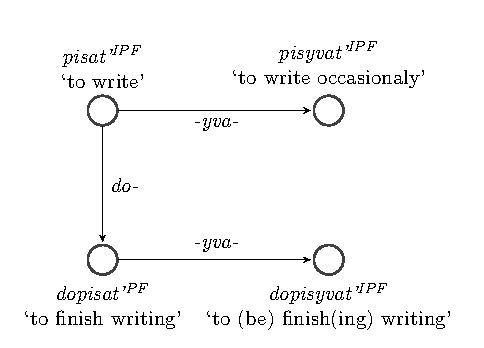
\includegraphics{graphPisat.pdf}
\caption{A fragment of the derivational graph: \textit{pisat'} `to write'\label{tree:dopisyvat}}
\end{figure}

The fragment of the \isi{derivational graph}, presented on \figref{tree:dopisyvat}, provides evidence for the hypothesis that, if a verb contains both the prefix \Prefix{do-} and the \isi{imperfective suffix}, it is imperfective. However, this hypothesis is quickly rejected on the basis of the other part of the graph: if one searches through the paths from the verb \textit{pisat'} `to write' to the verb \textit{dozapisyvat'} `to finish/be finishing writing down/recording', one finds two different \isi{derivational chains} in the \isi{derivational graph}, as shown in \figref{tree:dozapisyvat}. The first \isi{derivational chain}, linearised in \ref{deriv:dozapisyvat1}, provides evidence against the proposed hypothesis, as the verb at the end of this chain is perfective and contains both the \isi{imperfective suffix} and the prefix \Prefix{do-}.\largerpage[-1]

\ex.\label{deriv:dozapisyvat}\ag.\label{deriv:dozapisyvat1}pisat'\textsuperscript{\IPF} $\rightarrow$ zapisat'\textsuperscript{\PF} $\rightarrow$ zapisyvat'\textsuperscript{\IPF} $\rightarrow$ dozapisyvat'\textsuperscript{\PF}\\
{to write} $\rightarrow$ {to record} $\rightarrow$ {to (be) record(ing)} $\rightarrow$ {to finish recording}\\
\bg.\label{deriv:dozapisyvat2}pisat'\textsuperscript{\IPF} $\rightarrow$ zapisat'\textsuperscript{\PF} $\rightarrow$ dozapisat'\textsuperscript{\PF} $\rightarrow$ dozapisyvat'\textsuperscript{\IPF}\\
{to write} $\rightarrow$ {to record} $\rightarrow$ {to finish recording} $\rightarrow$ {to (be) finish(ing) recording}\\				

\begin{figure}
\begin{center}
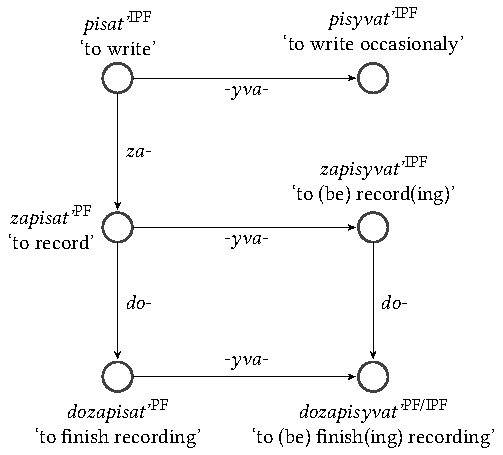
\includegraphics[scale=1]{graphDozapisyvat.pdf}
\caption{A fragment of the derivational graph: \textit{pisat'} `to write' and \textit{dozapisyvat'} `to (be) finish(ing) recording'\label{tree:dozapisyvat}}
\end{center}
\end{figure}			

The example above is just one illustration of how a \isi{derivational graph} defined by \defref{def:chain} can be used to check possible generalisations about the properties of Russian prefixed verbs. Such a graph, however, does not exist in the form of a human-created resource\footnote{The graph itself exists by definition, so what I mean here is some resource that stores this graph and allows to extract information from it.} and some researchers doubt even the possibility of writing it down in an overt form. For example, \citet[625]{Janda:07a} claims that ``exhaustive listings of verbs would be unwieldy, and, given the ad-hoc open-class nature of Specialised Perfectives and Complex Acts, such lists could never be definitive''. \citet[626]{Janda:07a} also regards most of the verbs that are not listed in the dictionaries and constructed spontaneously by the speakers not to be a core part of the \isi{verbal cluster}.

I do not agree with the claim about the marginal status of such verbs and consider them one of the core components of the Russian verbal system. Moreover, I claim that there is a way to construct a \isi{derivational graph} defined above. To do this, I propose to take the following approach: I base the generalisations in this and the following chapters on the data about parts of this graph that are built using introspection and corpora/search engine data. Afterwards, in Chapters~\ref{Chapter7} and \ref{Chapter8}, I propose a formal account that is capable of predicting which vertices and edges, apart from those already included on the basis of dictionary data, should be added to the \isi{derivational graph} (at the moment only with respect to the five prefixes I analyse in this work). I also check these predictions at least partially against corpora and search engine data. The output of the computational system I propose can later be used to build a larger version of the \isi{derivational graph}. An implemented database that is constructed on the basis of the dictionary data, such as OSLIN, can serve as a starting point for the proposed construction.

\subsection{Predicting the aspect of the derived verb}\label{subsection:predict}
As discussed in Section~\ref{subsection:bi:predictions}, the property that drives the analysis proposed here and is implicitly rejected by the \isi{syntactic theories} of Russian \isi{prefixation} is that a given verb does not need to be associated with a unique \isi{derivational chain}. For example, the biaspectual verb \textit{dozapisyvat'} `to (be) finish(ing) recording/writing down' appears as the last node of two \isi{derivational chains} given in \ref{deriv:dozapisyvat}, where one of them motivates the perfective aspect of the whole verb \ref{deriv:dozapisyvat1}, while the other motivates the imperfective aspect of the same verb \ref{deriv:dozapisyvat2}.

For a verb to have two \isi{derivational chains} implies that it may be \isi{ambiguous with respect to grammatical aspect}: each \isi{derivational chain} yields exactly one grammatical aspect for the derived verb, either perfective or imperfective. The \isi{context} then presumably selects one of the \isi{derivational chains}, and consequently, either the perfective or imperfective aspect of the verb, contrary to the syntactic approaches (in their existing form), which can only provide one \isi{derivational chain} for any given complex verb form due to formal restrictions on the positions of different affixes.

This is desirable given that, judging from the data, the verb \textit{dozapisyvat'} `to (be) finish(ing) recording/writing down' is genuinely ambiguous with respect to the perfective/imperfective distinction, and it is the \isi{context} that enforces one or the other grammatical aspect assignment. Note that the two \isi{derivational chains} in \ref{deriv:dozapisyvat1} and \ref{deriv:dozapisyvat2}, discussed above, straightforwardly follow from the two general patterns that are widely accepted as governing the formation of Russian verbs, although there are also some exceptions to them that will be discussed in Section~\ref{section:new:perfectivity}:

\begin{enumerate}
\item the output of a \isi{prefixation} is perfective;   
\item adding the \isi{imperfective suffix} to a verb yields an imperfective verb. 
\end{enumerate}

The root verb in \ref{deriv:dozapisyvat1} and \ref{deriv:dozapisyvat2} is the primary imperfective verb \textit{pisat'} `to write/to be writing'. Adding the prefix \textit{za}- to it yields a perfective verb, in compliance with (1), and the attachment of the \isi{imperfective suffix} -\textit{yva}- yields a \isi{secondary imperfective} verb, following (2). This verb in turn serves as the basis for the \isi{prefixation} with the \isi{completive} prefix \Prefix{do-}. The result is the perfective verb \textit{dozapisyvat'} `to finish recording/writing down', in compliance with (1).  In \ref{deriv:dozapisyvat2}, the second and the third steps are reversed, leading to the imperfective category assignment to the derived verb \textit{dozapisyvat'} `to finish/be finishing recording/writing down'.

Let me explain why the approach outlined here leads to different predictions than the syntactic accounts despite the fact that in both cases it is the final step of the derivation that determines the aspect of the whole complex verb. The crucial assumption of the syntactic approaches to \isi{prefixation} in Russian is that each prefix (with fixed interpretation) occupies a particular position in the \isi{syntactic tree}. From this it follows that structural properties of the verbs that have the same outermost prefixes are always the same. For example, the verbs that we have just considered, \textit{dopisyvat'}\textsuperscript{\IPF} `to (be) finish(ing) writing' and \textit{dozapisyvat'}\textsuperscript{\IPF\slash\PF} `to finish/be finishing recording/writing down', are either both perfective or both imperfective on any existing syntactic \isi{prefixation} account, as they contain the same outermost prefix \Prefix{do-} and its position in the tree determines the aspect of the whole verb. On the account advocated here, there is an evident difference between these verbs, as the order of the derivational steps is determined based on all possible \isi{derivational chains} that are constructed in compliance with \defref{def:history}. While the verb \textit{dozapisyvat'}\textsuperscript{\IPF\slash\PF} `to (be) finish(ing) writing down/recording' has two \isi{derivational chains}, as has been shown by \ref{deriv:dozapisyvat1} and \ref{deriv:dozapisyvat2}, which motivates its \isi{biaspectual nature}, the imperfective verb \textit{dopisyvat'}\textsuperscript{\IPF} `to finish/be finishing writing' has only one, as has been shown by \ref{deriv1}, so it can be only assigned the imperfective aspect.

Another example, already mentioned in Section~\ref{subsection:bi:apply}, is the verb \textit{dovy\v{s}ivat'} `to finish embroidering'. It contains the same type of affixes as the verb \textit{dozapisyvat'} `to finish recording/writing down'. Namely, a \isi{completive} prefix \Prefix{do-}, one more prefix commonly characterised as a \isi{lexical prefix}, and the \isi{imperfective suffix}. The verbs \textit{dovy\v{s}ivat'} `to finish embroidering' and \textit{dozapisyvat'} `to finish recording/writing down' are morphologically alike and thus there is no structural difference between them on any existing syntactic account of Russian verbal \isi{prefixation}, as the structure of the verb and the order of the affix attachment is determined only on the basis of the syntactic properties of the affixes (with fixed interpretation).\largerpage
 
It turns out that these verbs are clearly different for most native speakers: while the perfective uses of the verb \textit{dozapisyvat'} `to finish recording/writing down' may be judged odd by some speakers (as claimed by Sergei Tatevosov, personal communication\footnote{Note that such behaviour can be explained on the account proposed here by assuming that these speakers use a stronger version of a general \isi{pragmatic principle} that is used to account for the non-existence of a range of verbs (more information in Chapters~\ref{Chapter5} and~\ref{Chapter6}). This principle says that a more complex morphological form cannot be used to express the same meaning that a less marked form has. As a default, the domain of available \isi{alternatives} is restricted to the verbs belonging to one \isi{derivational chain} (where the complexity is directly connected to the place in the chain). In the stronger version, however, one can widen the domain to all the chains that start from the same source node. This modification will allow to account for the variation in the acceptability of various verbs.}), all the native speakers that I have consulted with agree that the verb \textit{dovy\v{s}ivat'} `to finish embroidering' can be used as a perfective verb. Moreover, most of these speakers do not accept \textit{dovy\v{s}ivat'} `to finish embroidering' as an imperfective verb. The same group of people rejects the existence of the verb $^?$\textit{dovy\v{s}it'}\textsuperscript{\PF} `to finish embroidering'. This behaviour is easily explained by means of the relevant part of the \isi{derivational graph}, presented on \figref{tree:dovyshivat}. For the group of speakers who reject the existence of the verb $^?$\textit{dovy\v{s}it'}\textsuperscript{\PF} `to finish embroidering', the derivation in \ref{deriv:dovyshivat2} is not available, as it requires the verb $^?$\textit{dovy\v{s}it'}\textsuperscript{\PF} `to finish embroidering' to be attested. Thus the verb \textit{dovy\v{s}ivat'} `to finish embroidering' cannot be assigned the imperfective aspect. On the other hand, at least some of the speakers that accept the verb $^?$\textit{dovy\v{s}it'}\textsuperscript{\PF} `to finish embroidering' also have access to the imperfective aspect of the verb \textit{dovy\v{s}ivat'} `to finish embroidering'.

\ex.\label{deriv:dovyshivat}\ag.\label{deriv:dovyshivat1}\v{s}it'\textsuperscript{\IPF} $\rightarrow$ \Prefix{vy-}\v{s}it'\textsuperscript{\PF} $\rightarrow$ \Prefix{vy-}\v{s}-iva-t'\textsuperscript{\IPF} $\rightarrow$ \Prefix{do-}\Prefix{vy-}\v{s}-iva-t'\textsuperscript{\PF}\\
{to sew} $\rightarrow$ {to embroider} $\rightarrow$ {to embroider/be embroidering} $\rightarrow$ {to finish embroidering}\\
\bg.\label{deriv:dovyshivat2}\v{s}it'\textsuperscript{\IPF} $\rightarrow$ \Prefix{vy-}\v{s}it'\textsuperscript{\PF} $\rightarrow$ \Prefix{do-}\Prefix{vy-}\v{s}it'\textsuperscript{\PF} $\rightarrow$ \Prefix{do-}\Prefix{vy-}\v{s}-iva-t'\textsuperscript{\IPF}\\
{to sew} $\rightarrow$ {to embroider} $\rightarrow$ {to finish embroidering} $\rightarrow$ {to finish/be finishing embroidering}\\

\begin{figure}
\begin{center}
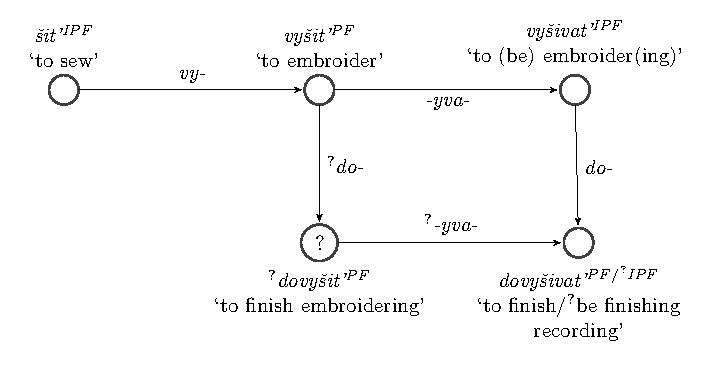
\includegraphics[scale=1]{graphDovyshivat.pdf}
\caption{A fragment of the derivational graph: \textit{\v{s}it'} `to sew' and \textit{dovy\v{s}ivat'} `to finish embroidering'\label{tree:dovyshivat}}
\end{center}
\end{figure}		

I would like to also point out another question that naturally arises in connection with the possible paths in the \isi{derivational graph}. One may ask whether there are prefixes that can be considered perfectivity markers. The first step towards answering this question would be to look for a prefix such that whenever a verb contains it, there are no outgoing edges from the node corresponding to this verb in the \isi{derivational graph}. Although this is a reformulation of one of the classical characteristics of the \isi{superlexical} prefixes,\footnote{See, e.g. \citet{Ramchand:04}, \citet{Svenonius:04a}, and \citet{Romanova:06}, who assume that \isi{superlexical} prefixes occupy the highest position in the verbal structure.} \citet{Tatevosov:07, Tatevosov:09} provides numerous counterexamples to such a constraint. In the account proposed in \citealt{Tatevosov:09}, the main constraints on the attachment of the \isi{superlexical} prefixes are formulated in different terms: they must be attached either before the \isi{imperfective suffix} or to a formally imperfective verb. Only the \isi{distributive} prefix \textit{po}- that, according to \citet{Tatevosov:09}, occupies the \isi{left periphery} of the verb, is then a prefix of such a type that the verb that contains it is necessarily perfective and no other morpheme can be attached higher than it. I will further investigate the ability of the individual prefixes discussed here to constitute a part of an imperfective verb in Chapter~\ref{Chapter5}.\footnote{Note that even if we find such prefixes that can be encountered only on the last derivational step, they are not necessarily perfectivity markers, as there may be other reasons (e.g. semantic, pragmatic, phonological) why further derivational steps are not possible.}

\section{Prefixation and perfectivity}\label{section:new:perfectivity}

\subsection{Introduction}
It is generally assumed in Russian morphology that, if the last step of the verbal derivation is \isi{prefixation}, the verb comes out perfective. This fact does not depend on the point where the perfectivity comes in: in both aspect-low \citep[][among others]{Verkuyl:95, Pinon:01, Ramchand:04} and aspect-high \citep{Paslawska:03, Gronn:10, Tatevosov:11} theories, prefixes carry some property that either immediately or later leads to the perfective aspect of the verb. In this section we will discuss cases that seem to provide exceptions to this pattern.

In the first part, Section~\ref{subsection:perf:borrowed}, we will look at the \isi{prefixation} of \isi{borrowed biaspectual verbs} with native prefixes. Then, in Section~\ref{subsection:perf:imperf}, we will examine what happens if an imperfective verb derived from a borrowed root gets prefixed. Next, in Section~\ref{subsection:perf:native}, we will discuss the case of native \isi{biaspectual verbs} and their \isi{prefixation}. The discussion will be followed by some information on borrowed prefixes, as they do not affect the aspect of the verb they are attached to (Section~\ref{subsection:perf:prefixes}). We will then close with considering the problem of motion verbs that are often said to resist \isi{perfectivisation} when prefixed (Section~\ref{subsection:perf:motion}, also published as \citealt{ZinovaOsswald:paper}).

\subsection{Prefixation of borrowed biaspectual verbs}\label{subsection:perf:borrowed}
Consider the verbs \textit{perezapisat}'\textsuperscript{\PF} `to rerecord' and \textit{zapisyvat'}\textsuperscript{\IPF} `to  record/be recording'. Both verbs are attested and commonly used by native speakers. Intuitively, the verb \textit{perezapisyvat'} `to rerecord/be rerecording' can be formed from either of them: one can add the \isi{imperfective suffix} to the verb \textit{perezapisat}'\textsuperscript{\PF} `to rerecord' or the \isi{repetitive} prefix \Prefix{pere-} to the verb \textit{zapisyvat'}\textsuperscript{\IPF} `to (be) record(ing)'. This is schematically shown in \ref{schema:perezapisyvat'}.

\ex.\label{schema:perezapisyvat'}\ag.\label{schema:perezapisyvat'1}pisat'\textsuperscript{\IPF} {$\rightarrow$} zapisat'\textsuperscript{\PF} {$\rightarrow$} perezapisat'\textsuperscript{\PF} {$\rightarrow$} perezapisyvat'\textsuperscript{\IPF} \\
{`to write'} {} {`to record'} {} {`to rerecord'} {} {`to rerecord/be rerecording'}\\
\bg.\label{schema:perezapisyvat'2}pisat'\textsuperscript{\IPF} {$\rightarrow$} zapisat'\textsuperscript{\PF} {$\rightarrow$} zapisyvat'\textsuperscript{\IPF} {$\rightarrow$} perezapisyvat'\textsuperscript{\IPF} \\
{`to write'} {} {`to record'} {} {`to record/be recording'} {} {`to rerecord/be rerecording'}\\

The \isi{derivational chain} in \ref{schema:perezapisyvat'2} is excluded under all accounts for verbal \isi{prefixation}, since it violates the assumption that adding a prefix as a last derivational step makes the derived verb perfective. However, on the intuitive level, the derivation in \ref{schema:perezapisyvat'2} is acceptable. This leads to us to question the hypothesis of a uniform perfectivising function of all the verbal prefixes in Russian. In order to address this question, we have to look at some derivations where there is no potential for switching the order of the derivational steps.

A case in point are \isi{borrowed biaspectual verbs}. Consider the biaspectual verb \textit{kvalificirovat'} `to qualify/to classify'. It is formed with the native verbal suffix -\textit{irova}-, which instantiates one of the systematic patterns of formation of borrowed verbs. This verb can be prefixed with the \isi{repetitive} prefix \Prefix{pere-}. The result of such a \isi{prefixation} is the verb \textit{perekvalificirovat'} `to requalify/to recategorise', which is, in turn, also biaspectual.

In order to show that in this case \isi{prefixation} does not lead to the perfective aspect of the verb, I have to prove two things: (1) that the verb \textit{perekvalificirovat'} `to requalify/to recategorise' is indeed biaspectual and (2) that there is no other way to derive the verb \textit{perekvalificirovat'} `to requalify/to recategorise' than by attaching the prefix \Prefix{pere-} to the verb \textit{kvalificirovat'} `to qualify/to classify'.

To show that the prefixed verb \textit{perekvalificirovat'} `to requalify/to reclassify' is  biaspectual, let me provide evidence of its usage both as a perfective and as an imperfective verb. Example \ref{ex:perekvalificirovat:perf} illustrates the usage of the verb \textit{perekvalificirovat'} `to requalify/to reclassify' in the perfective aspect and the constructed sentence \ref{ex:perekvalificirovat:perf2} shows that perfective aspect is available according to the test offered in Section~\ref{sec:tests:new}.

\ex.\ag.\label{ex:perekvalificirovat:perf}Krome togo, vynosja prigovor, sud'ja perekvalificiroval\textsuperscript{\PF} obvinenie i snizil s ``osobo krupnogo'' na ``krupnyj'' objem nefti, v xi\v{s}\v{c}enii kotoroj obvinjajutsja podsudimye.\\
apart this, vy.carry.\glb{part.pres} sentence.\glb{sg.acc} judge.\glb{sg.nom} pere.classify.\glb{pst.sg.m} accusation.\glb{sg.acc} and lower.\glb{pst.sg.m} from ``particularly large'' on ``large'' volume.\glb{sg.acc} oil.\glb{gen} in theft.\glb{sg.prep} which.\glb{f.sg.prp} accuse.\glb{pres.3.pl.}refl defendant.\glb{pl.nom}\\
\trans `Apart from this, when pronouncing the sentence, the judge reclassified the accusation, changing the amount of oil that the defendants are accused of stealing from ``particularly large'' into ``large''.'\\
\hbox{}\hfill\hbox{\url{https://www.vesti.ru/article/2093393}, accessed on 03.08.2021}
\bg.\label{ex:perekvalificirovat:perf2}Sud'ja perekvalificiroval\textsuperscript{\PF} delo i po\v{s}\"{e}l domoj.\\
judge.\glb{sg.nom} pere.classify.\glb{pst.sg.m} case.\glb{sg.acc} and po.go.\glb{pst.sg.m} home\\
\trans `The judge reclassified the case and went home.'

To show that the verb \textit{perekvalificirovat'} `to requalify/to reclassify' can also be used as an imperfective verb, I apply to it the four common tests that delimit \isi{imperfective verbs}. It turns out that in an appropriate \isi{context} the verb \textit{perekvalificirovat'} `to requalify/to reclassify' can have a \isi{progressive interpretation}, as shown by example \ref{ex:qualify1}, it can be used as a complement of a \isi{phasal verb}, as in \ref{ex:qualify2}, form periphrastic \isi{future}, as in the sentence \ref{ex:qualify3}, and form a \isi{present participle}, as in \ref{ex:qualify4}. 

\ex.\label{ex:qualify}\ag.\label{ex:qualify1}V dannyj moment on perekvalificiruet\textsuperscript{\IPF} svoju {``Armiju Maxdi''} v politi\v{c}eskoe dvi\v{z}enie.\\
in given moment he pere.qualify.\glb{pres.3.sg} his {``Armija Maxdi''} in political movement\\
\trans `Right now he is re-categorising his ``Armija Maxdi'' into a political movement.'\hbox{}\hfill\hbox{\url{https://www.km.ru/glavnoe/2005/06/14/politika/rossiiskii-posol-v-irake-vstretilsya-s-muktadoi-sadrom}, accessed on 03.08.2021}
\bg.\label{ex:qualify2}Sej\v{c}as advokaty na\v{c}nut perekvalificirovat'\textsuperscript{\IPF} delo v politi\v{c}eskoje.\\
now advocates start.\glb{pres.3.pl} iter.qualify.\glb{inf} case in political\\
\trans `Now the advocates will start to re-classify this case as a political one.'\hfill\hbox{\url{https://pikabu.ru/story/v_polshe_zaderzhali_prokurora_ignatenko_396297/author}, accessed on 03.08.2021}
\bg.\label{ex:qualify3}Policejskix budut perekvalificirovat'\textsuperscript{\IPF} v buxgalterov.\\	
policemen will.be pere.qualify\glb{.inf} in accountant.\glb{pl.acc}\\
\trans `Policemen will be re-trained and become accountants.'\hbox{}\hfill\hbox{\url{https://pikabu.ru/story/politseyskikh_budut_perekvalifitsirovat_v_bukhgalterov_169505}, accessed on 03.08.2021}
\bg.\label{ex:qualify4}Ne pozvoljaetsja smotret’ na perekvalificiruemye sdelki s pozicii togo, \v{c}to nalogoplatel’\v{s}\v{c}ik mog sdelat’ v tex uslovijax.\\
not allow look on pere.qualify.\glb{part.pres.pl.acc} deals from position that, that tax.payer can.\glb{pst.sg.m} s.do.\glb{inf} in that conditions\\
\trans `We cannot view the deals which are subject to reclassification on the basis of what a tax-payer would have done under the same circum\-stances.'\hbox{}\hfill\hbox{\url{http://lesregion.ru/main/1455-osobennosti-rascheta-summy-nds-iznutri-summy-sdelki-pri-ee-nalogovoy-perekvalifikacii.html}, accessed on 03.08.202}

Now let us examine other potential ways of deriving the verb \textit{perekvalificirovat'} `to requalify/to reclassify' such that \isi{prefixation} is not the last derivational step. The first idea is to allow the possibility of the suffix \is{suffix!-ova-}\textit{-ova-} to be attached after the prefix \Prefix{pere-}. This is not possible, since there is no verb *\textit{kvalificirit'} (i.e., \textit{kvalificirovat'} without the suffix -\textit{ova}-) and also no verb  *\textit{perekvalificirit'} that can be imperfectivised by the addition of the \isi{imperfective suffix}.

Another possibility that must be considered is illustrated by \ref{chain:kvalificirovat'}. In this potential \isi{derivational chain}, the verb \textit{kvalificirovat'} `to qualify/to classify' is first turned into the noun \textit{kvalifikacija} `qualification\slash classification', then the noun is prefixed with the prefix \Prefix{pere-} to obtain the noun \textit{perekvalifikacija}  `requalification/reclassification' (example \ref{ex:kvalifikacija} illustrates its usage) and then the verb \textit{perekvalificirovat'} `to requalify/to reclassify' is derived from this noun. 
\exg.\label{chain:kvalificirovat'}kvalificirovat'\textsuperscript{\PF\slash\IPF} {$\rightarrow$} kvalifikacija {$\rightarrow$} perekvalifikacja {$\rightarrow$} {perekvalificirovat'\textsuperscript{\PF\slash\IPF}}\\
{`to qualify'} {} {`qualfication'} {} {`requalification'} {} {`to requalify'}\\

\exg.\label{ex:kvalifikacija}Process trudoustrojstva mo\v{z}et uprostit' perekvalifikacija.\\
process.\glb{sg.acc} placement.\glb{sg. gen} can.\glb{pres.3.sg} simplify.\glb{inf} pere.qualification.\glb{sg.nom}\\
\trans `The re-training can simplify the process of placement.'\\\hbox{}\hfill\hbox{\url{http://worldofscience.ru/menedzhment.html?start=120}, accessed on 03.08.2021}

The chain in \ref{chain:kvalificirovat'} should be compared with \ref{chain:kvalifikacija}, where the \isi{prefixed noun} is derived from the prefixed verb, and not vice versa, but requires us to assume a \isi{non-perfectivising} usage of the prefix \Prefix{pere-}.

\exg.\label{chain:kvalifikacija}kvalificirovat'\textsuperscript{\PF\slash\IPF} {$\rightarrow$} {perekvalificirovat'\textsuperscript{\PF\slash\IPF}} {$\rightarrow$} perekvalifikacja\\
{`to qualify'} {} {`to requalify'} {} {`requalification'}\\

Each of the steps of the proposed derivation in \ref{chain:kvalificirovat'} is attested in the Russian derivational morphology. The noun \textit{kvalifikacija} `qualification\slash classification' is no doubt derived from the verb \textit{kvalificirovat'} `to qualify/to classify'. \citet{Shvedova:82} writes in this respect that nouns with the suffix \textit{-acij-} are motivated mostly by the borrowed verbs with the stem ending in \textit{-irovat'}. Examples \citep[taken from][159]{Shvedova:82} include the following pairs: \textit{simulirovat'} `to feign' -- \textit{simuljacija} `simulation', \textit{idealizirovat'} `to idealise'  -- \textit{idealizacija} `idealization', \textit{abstragirovat'} `to abstract' -- \textit{abstrakcija} `abstraction'.

The second step, \isi{prefixation} of the noun \textit{kvalifikacija} `qualification\slash classifica\-tion' with the prefix \Prefix{pere-}, is also allowed by the Russian morphological system: \citet[226]{Shvedova:82} writes that nouns that formed with the prefix \Prefix{pere-} ``nazyvajut povtornost' dejstvija ili javlenija, nazvannogo motiviruju\v{s}\v{c}im slovom'' [name the \isi{repetition} of an action or a phenomenon that is named by the motivating word].

The third step, derivation of a verb ending in \textit{-irovat'} from the noun, is also a possible \isi{morphological operation} in Russian. For example, in the pair \textit{sklad} `warehouse' -- \textit{skladirovat'}\textsuperscript{\PF\slash\IPF} `to store' the verb is obtained by \isi{suffixation} of the noun and it is biaspectual.

So far it seems that the derivation in \ref{chain:kvalificirovat'} is a possible one. To test this hypothesis further, let us consider the \isi{completive} prefix \Prefix{do-}. Analogously to the noun \textit{perekvalifikacija} `requalification/reclassification' and the verb \textit{perekvalificirovat'} `to requalify/to reclassify', there exist a noun \textit{dokvalifikacija} `qualification improvement', as in \ref{ex:dokvalifikacija}, and a verb \textit{dokvalificirovat'} `to improve qualification'. If the derivation in \ref{chain:kvalificirovat'} is a valid derivation, so must be the one in \ref{chain:dokvalificirovat'}.

\exg.\label{ex:dokvalifikacija}Avtoservis primet na rabotu avto\`{e}lektrika. V perspektive vozmo\v{z}na dokvalifikacija.\\
{auto.service} take.\glb{pres.3.sg} on work {auto.electrician.\glb{sg.acc}} in perspective possible do.qualification.\glb{sg.nom}\\
\trans `Auto service is hiring an auto electrician. Future additional training possible.' \hfill\hbox{\url{https://forum.novgorod.ru/q92686.html}, accessed on 03.08.2021}

\exg.\label{chain:dokvalificirovat'}kvalificirovat'\textsuperscript{\PF\slash\IPF} {$\rightarrow$} kvalifikacija {$\rightarrow$} dokvalifikacja {$\rightarrow$} dokvalificirovat'\textsuperscript{\PF\slash\IPF}\\
{`to qualify'} {} {`qualfication'} {} {`qualification improvement'} {} {`to improve qualification'}\\

It is obvious that the verb \textit{dokvalificirovat'} `to improve qualification' can be used as a perfective verb, as in \ref{ex:dokvalificirovat':perf}. The surprising part is that some speakers accept it also as an imperfective verb. Examples of the imperfective usage of this verb are found on the internet: the verb \textit{dokvalificirovat'} `to improve qualification' can have a \isi{progressive interpretation} \ref{ex:dokvalificirovat':ongoing} and form a \isi{present participle} \ref{ex:dokvalificirovat':part} and periphrastic \isi{future} \ref{ex:dokvalificirovat':future}. 

\exg.\label{ex:dokvalificirovat':perf}Ja okon\v{c}il Veterinarnuju akademiju, a armija dokvalificirovala menja do normal'nogo medika.\\
I finish.\glb{pst.sg.m} veterinary.\glb{f.sg.acc} academy.\glb{sg.acc}, but army.\glb{sg.nom} do.qualify.\glb{pst.sg.f} me.\glb{acc} to normal.\glb{m.sg.gen} physician.\glb{sg.gen}\\
\trans `I graduated from the vererinary academy and in the army I improved my qualification enough to become a physician.'\hbox{}\hfill\hbox{\url{https://www.kommersant.ru/doc/2288059}, accessed on 03.08.2021}

\ex.\label{ex:dokvalificirovat':imperf}\ag.\label{ex:dokvalificirovat':ongoing}My vs\"{e} vremja u\v{c}im, pereobu\v{c}aem na\v{s}i kadry, dokvalificiruem, perekvalificiruem.\\
we all time teach.\glb{pres.3.sg}, pere.ob.teach.\glb{pres.3.sg} our personnel.\glb{pl.acc}, do.qualify.\glb{pres.3.sg}, pere.quaify.\glb{pres.3.sg}\\
\trans `We always teach and reteach our personnel, train them to the new levels, re-train them.'\hbox{}\hfill\hbox{\url{http://rus-yaz.niv.ru/doc/gallism-dictionary/fc/slovar-202-15.htm}, accessed on 03.08.2021}
\bg.\label{ex:dokvalificirovat':part}Pri \`{e}tom kak nastavnikam novoprinjatyx kolleg, tak i dokvalificiruemyx proizvoditsja premial'naja oplata za rabo\v{c}ee vremja, posvja\v{s}\v{c}ennoe obu\v{c}eniju.\\
with this as mentor.\glb{pl.dat} new.accepted.\glb{pl.gen} colleague.\glb{pl.gen}, so and do.qualify.\glb{part.pass.pres.pl.gen} make.\glb{pres.3.sg.}refl premium payment.\glb{sg.nom} behind work.\glb{sg.n.acc} time.\glb{sg.acc}, dedicate.\glb{part.pass.pst.sg.n.nom} education.\glb{dat}\\
\trans `Wherein both mentors of the new recruits as well as mentors of those workers that are being given extra-trained are paid additionally for the working time they spend on educational purposes.'\\\hbox{}\hfill\hbox{\url{https://kurs.znate.ru/docs/index-170298.html?page=5}, accessed on 03.08.2021}
\bg.\label{ex:dokvalificirovat':future}Kto budet dokvalificirovat' kadry?\\
Who will do.qualify.\glb{inf} personnel.\\
\trans `Who will train the personnel to the new level?'\\\hbox{}\hfill\hbox{\url{https://twitter.com/hashtag/smartcitykazan}}

\largerpage As there are few examples like these in \ref{ex:dokvalificirovat':imperf} on the internet, I have run a mini-survey, asking native speakers of Russian if the sentences in \ref{ex:dokvalificirovat':imperf} are acceptable for them. Out of 11 respondents, 4 accepted \textit{dokvalificirovat'} `to improve qualification' as an imperfective verb, while 7 did not.

What some speakers suggested was to attach the \isi{imperfective suffix} to the verb \textit{dokvalificirovat'} `to improve qualification', which they consider exclusively perfective, and derive the imperfective verb \textit{dokvalificirovyvat'} `to improve qualification', as in \ref{ex:dokvalificirovyvat}). 

\exg.\label{ex:dokvalificirovyvat}Vodil nado dokvalificirovyvat' v vy\v{s}ibal, \v{c}tob oni prinimali v takix slu\v{c}ajax kardinal'nye mery.\\
driver.\glb{pl.acc} need do.qualify.imp.\glb{inf} in doorman.\glb{pl.acc}, that they take.\glb{pst.pl} in such case.\glb{pl.prp} drastic measure.\glb{pl.acc}\\
\trans `Drivers should be re-trained as bouncers, so that they could take drastic measures.'\hbox{}\hfill\hbox{\url{journals.ru}}

The derived verb is not very natural from a phonological point of view and hardly used. \citet[590]{Shvedova:82} writes that \isi{suffixation} with \textit{-iva-} is possible for the verbs with the \is{suffix!-ova-}\textit{-ova-/-irova-} suffix only if the last syllable of the suffix is stressed.\footnote{\citet[590]{Shvedova:82}: ``pribavlenie morfa \textit{-­iva-} vozmo\v{z}no tol'ko v tom slu\v{c}ae, kogda udarenie padaet na vtoroj slog suf. \textit{-­ova-/-irova-}'' [the addition of the \textit{-iva-} morpheme is possible only if the second syllable of the \textit{-­ova-/-irova-} suffix is stressed], but from the examples that follow it is clear the she means either the second syllable of the \textit{-ova-} suffix or the last syllable of the \is{suffix!-ova-}\textit{-irova-} suffix.} In sum, it seems that \isi{imperfectivisation} with the suffix \textit{-iva-} is allowed from a morphological point of view, but blocked for phonological reasons.
 
A behaviour similar to the one of \Prefix{do-} is observed for the prefix \Prefix{pod-}. Consider, for example, the borrowed biaspectual verb \textit{amortizirovat'} `to cushion'. The verb \textit{podamortizirovat'} `to cushion slightly' can be grammatically perfective verb, as in \ref{ex:cushion1}, or, in some cases like \ref{ex:cushion2}, imperfective. Again, there exists a noun \textit{podamortizacija} `slight cushioning', as in \ref{ex:podamortizacija}, that could serve as a source of derivation of the prefixed verb, but is accepted only by some native speakers of Russian.

\ex.\label{ex:cushion}\ag.\label{ex:cushion1}…krome togo, mo\v{z}no e\v{s}\v{c}e snizu porolon\v{c}ikom \v{z}\"{e}stkim podamortizirovat'\textsuperscript{\PF}\\		
…aside that, possible also below {foam rubber} hard pod.cushion.\glb{inf}\\
\trans `it is also possible to put some hard foam rubber below as a cushion'\\\hbox{}\hfill\hbox{\url{forum.guitarplayer.ru}}
\bg.\label{ex:cushion2}\v{C}to tolku podamortizirovat'\textsuperscript{\IPF} perednee koleso, esli zadnie \v{z}estko sidjat na rame.\\
what sense pod.cushion.\glb{inf} front wheel if back hardly sit.\glb{pres.pl} on frame\\
\trans `What's the point to cushion the front wheel when the back ones are sitting hard on the frame?'\hbox{}\hfill\hbox{\url{www.pnevmohod.ru}}

\exg.\label{ex:podamortizacija}Ili, ska\v{z}em, v BTR-ax su\v{s}\v{c}estvuet podamortizacija sidenij: dlja togo, \v{c}toby v slu\v{c}ae naezda na minu desantnika ne tak sil'no trjaxnulo.\\
Or, say.\glb{pres.1.pl}, in BTR.\glb{pl.prep} exist.\glb{pres.3.sg} pod.cushioning.\glb{sg.nom} seat.\glb{pl.gen}: for that, that in case hitting on bomb paratrooper not as strongly shake.\glb{pst.sg.n}\\
\trans `Or, say, BTRs have a slight seat cushioning: so if it drives over a bomb the paratrooper won't be shaken so much.'\hbox{}\hfill\hbox{\url{topwar.ru}}

It might seem that for some speakers biaspectual borrowed verbs ending in \mbox{\textit{-irova}} lack aspect and remain underspecified in this respect when prefixed with any prefix. This is not the case, as apart from the three prefixes discussed above, \isi{biaspectual verbs} become perfective after \isi{prefixation}. 

As an example, let us consider the verb \textit{otkvalificirovat'} `to finish classifying'. It is formed by prefixing the verb \textit{kvalificirovat'} `to qualify/to classify' with the \isi{terminative} prefix \Prefix{ot-}. This verb can be only used as a perfective verb, as illustrated by \ref{ex:otkvalificirovat'}. Interestingly, in this case there is no noun *\textit{otkvalifikacija}, so a chain like the ones in \ref{chain:kvalificirovat'} and \ref{chain:dokvalificirovat'} cannot be constructed. 

\exg.\label{ex:otkvalificirovat'}Ja li\v{s} otkvalificiroval na osnovanii tipi\v{c}nyx voprosov.\\
I only ot.qualify.\glb{pst.sg.m} on basis typical question.\glb{pl.gen}\\
\trans `I only got re-qualified on the basis of the typical questions.'\\\hbox{}\hfill\hbox{\url{forum.nag.ru}}

It also has to be mentioned that, besides \isi{borrowed biaspectual verbs} with the \mbox{\textit{-irova}} suffix, there are also \isi{borrowed biaspectual verbs} with the suffix \is{suffix!-ova-}\textit{-ova-}, such as \textit{organizovat'} `to organise' in \ref{ex:organizovat1}.\largerpage[-1]

\exg.\label{ex:organizovat1}Pervyj kanal organizoval\textsuperscript{\PF} v Tule grandioznyj prazdnik dlja detej.\\
first channel organise.\glb{pst.sg.m} in Tula.\glb{prp} colossal celebration for children.\glb{gen}\\
\trans `Channel 1 organised a colossal celebration for children in Tula.'\\\hbox{}\hfill\hbox{\url{www.1tv.ru}}

The verb \textit{organizovat'} `to organise' does not fall under the \isi{phonological restriction} on the attachment of the \isi{imperfective suffix}, so an imperfective verb \textit{organizovyvat'}\textsuperscript{\IPF} `to organise/to be organising' does exist. Due to the presence of an unambiguously imperfective verb, \textit{organizovat'} `to organise' seems to be partially losing its biaspectuality, as I could find no examples of uttering \textit{organizovat'} `to organise' as an imperfective verb in the \isi{past} tense. However, in the non-\isi{past} tense imperfective usages of the verb \textit{organizovat'} `to organise' are natural and common (see example \ref{ex:organizovat}).

\exg.\label{ex:organizovat}Kak ja organizuju\textsuperscript{\IPF} informaciju pri prodvi\v{z}enii sajtov.\\
how I organise.\glb{pres.1.sg} information.\glb{acc} at promotion.\glb{sg.prp} website.\glb{pl.gen}\\
\trans `How do I organise information when promoting a website.'\hbox{}\hfill\hbox{shakin.ru}

This asymmetry may be due to the different ways of constructing the tensed forms of the verbs. In the \isi{past} tense, the personal forms of the verbs \textit{organizovat'} `to organise' and \textit{organizovyvat'}\textsuperscript{\IPF} `to organise/to be organising' differ by one syllable (\textit{organizoval} `he organised' vs. \textit{organizov\textbf{yv}al} `he organised/was organising'). In the non-\isi{past} tense, the phonological and \isi{morphological distance} is bigger: personal forms of the \isi{secondary imperfective} verb (e.g., \textit{organizo\textbf{vyva}ju} `I organise/am organising') are two syllables and two morphemes longer than the respective personal forms of the source verb (e.g., \textit{organizuju} `I organise'). Due to this, the cost of using the suffixed and not the original biaspectual verb (in a \isi{context} that requires the imperfective aspect) is less for the \isi{past} tense.

Both biaspectual and \isi{imperfective verbs} can be prefixed with the \isi{repetitive} prefix \Prefix{pere-}, producing the biaspectual verb \textit{pereorganizovat'} `to reorganise/be reorganising' and the imperfective verb \textit{pereorganizovyvat'} `to reorganise/be reorganising'. Potential \isi{derivational chains} for the imperfective verb \textit{pereorganizovyvat'} `to reorganise/be reorganising' are shown in \ref{chain:pereorg}. 

\ex.\label{chain:pereorg}\ag.organizovat'\textsuperscript{\PF\slash\IPF} {$\rightarrow$} {pereorganizovat'\textsuperscript{\PF\slash\IPF}} {$\rightarrow$} pereorganizovyvat'\textsuperscript{\IPF}\\
{`to organise'} {} {`to reorganise'} {} {`to reorganise/be reorganising'}\\
\bg.organizovat'\textsuperscript{\PF\slash\IPF} {$\rightarrow$} {organizovyvat'\textsuperscript{\IPF}} {$\rightarrow$} pereorganizovyvat'\textsuperscript{\IPF}\\
{`to organise'} {} {`to organise/be organising'} {} {`to reorganise/be reorganising'}\\

When the \isi{completive} prefix\largerpage\ \Prefix{do-} is attached to the same verbs, the verb \textit{doorganizovat'} `to finish organising' is clearly perfective and the verb \textit{doorganizovyvat'} `to finish/be finishing organising' is biaspectual, as evidenced by the examples in \ref{ex:doorganizovyvat}.

\ex.\label{ex:doorganizovyvat}\ag.sam budu doorganizovyvat'\textsuperscript{\IPF} obu\v{c}enie\\
myself will do.organise.imp.\glb{inf} education.\glb{acc}\\
\trans `I will finish organising the education process myself'\\\hbox{}\hfill\hbox{\url{deco-house.ru}}
\bg.Ja da\v{z}e svoju gil'diju do six por ne doorganizovyval\textsuperscript{\PF}, ne to, \v{c}to celoe kom'juniti\\
I also my guild.\glb{sg.acc} until this time not do.organise.imp.\glb{pst.sg.m}, not that, that whole community\\
\trans `I still have not finished organising my guild, let alone the whole community.'\hbox{}\hfill\hbox{\url{http://forum.tera-online.ru}}

\ex.\label{chain:doorg}\ag.organizovat'\textsuperscript{\PF\slash\IPF} {$\rightarrow$} {doorganizovat'\textsuperscript{\PF}} {$\rightarrow$} doorganizovyvat'\textsuperscript{\IPF}\\
{`to organise'} {} {`to finish organising'} {} {`to finish organising/be finishing organising'}\\
\bg.organizovat'\textsuperscript{\PF\slash\IPF} {$\rightarrow$} {organizovyvat'\textsuperscript{\IPF}} {$\rightarrow$} doorganizovyvat'\textsuperscript{\PF}\\
{`to organise'} {} {`to organise/be organising'} {} {`to finish organising/be finishing organising'}\\

If one compares the \isi{derivational chains} in \ref{chain:pereorg} and \ref{chain:doorg}, the difference between the behaviour of the prefix \Prefix{do-} and the behaviour of the prefix \Prefix{pere-} becomes evident: verbs containing the respective prefixes and not containing the extra \isi{imperfective suffix} have different aspectual characteristics. One may again try to adopt the path offered in \ref{chain:kvalificirovat'}: assume that biaspectual prefixed verb is formed on the basis of the \isi{prefixed noun} \ref{chain:pereorganizacija}.
 
\exg.\label{chain:pereorganizacija}organizovat'\textsuperscript{\PF\slash\IPF} {$\rightarrow$} organizacija {$\rightarrow$} pereorganizacija {$\rightarrow$} {pereorganizovat'\textsuperscript{\PF\slash\IPF}}\\
{`to organise'} {} `organisation' {} `reorganisation' {} {`to reorganise'}\\

It turns out that this hypothesis must be rejected. If \ref{chain:pereorganizacija} is a valid \isi{derivational chain}, so must be \ref{chain:doorganizacija}. In the latter case, however, the last verb in the chain, which is by hypothesis derived from the noun, lacks imperfective aspect. 

\exg.\label{chain:doorganizacija}organizovat'\textsuperscript{\PF\slash\IPF} {$\rightarrow$} organizacija {$\rightarrow$} doorganizacija {*$\rightarrow$} {doorganizovat'$^{{\PF}/^*{\IPF}}$}\\
{`to organise'} {} `organization' {} {`final stage of organization'} {} {`to finish organising'}\\

From this we have to conclude that the derivations \ref{chain:kvalificirovat'} and \ref{chain:dokvalificirovat'} do not seem to be empirically motivated and another explanation is needed. 

In sum, in this section I have shown that \isi{loaned} \isi{biaspectual verbs} exhibit unexpected behaviour when they are prefixed with one of the prefixes \Prefix{do-}, \Prefix{pere-}, and \Prefix{pod-}: they may remain biaspectual. This is especially prominent in the case of the prefix \Prefix{pere-} (with \isi{repetitive} interpretation) and less so in case of the prefixes \Prefix{do-} and \Prefix{pod-}. The \isi{non-perfectivising} behaviour of the prefix \Prefix{pere-} will be further discussed in Section~\ref{subsection:semantics:pere}. The cases where verbs prefixed with \Prefix{do-} remain biaspectual must be explained separately. Detailed investigation of this phenomena remains outside the scope of this book.\footnote{My primary hypothesis would be based on phonological considerations. I think that in these cases the formation of the \isi{secondary imperfective} from the prefixed borrowed biaspectual verb is possible from the point of view of both syntax and semantics. However, such forms are blocked for phonological reasons. One can hypothesise that in this case the less complex form (originally perfective) acquires the role of the blocked derivative (imperfective). I suppose that this is only possible when the suffix \is{suffix!-ova-}\textit{-ova-} marking borrowed verbs, that resembles the \isi{imperfective suffix}, is present.}
	
%In sum, there is a correlation between the existence of a \isi{prefixed noun} and the biaspectuality of the prefixed verb (only \isi{borrowed biaspectual verbs} ending in \textit{-irovat'} are considered here). This correlation is, however, not enough to conclude that \ref{chain:kvalificirovat'} and \ref{chain:dokvalificirovat'} are valid. It may be the case that the derivation of deverbal nouns is dependent on the derivation of a biaspectual prefixed verb, as nominalizations with the suffix \textit{-cij} are only possible if the source verb is imperfective or biaspectual. 

%In fact, this seems to be the most probable derivational variant. First reason is that it is more natural to assume the parallelism in the derivation of nouns with the suffix \textit{-cij-}: if \textit{kvalifikacija} `qualification/classification' is derived from \textit{kvalificirovat'} `to qualify/to classify', then it is likely that \textit{perekvalifikacija} `requalification/reclassification' is derived from \textit{rekvalificirovat'} `to requalify/to reclassify.' The second reason is that native speakers are less eager to accept the noun \textit{dokvalifikacija} `qualification improvement' than the verb \textit{dokvalificirovat'} `to improve qualification.'

\subsection{Prefixation of imperfective verbs with a borrowed root}\label{subsection:perf:imperf}
Let us now consider the verb \textit{planirovat'} `to plan/be planning'. It is an imperfective verb derived from the noun \textit{plan} `plan'. It turns out that the verb \textit{pereplanirovat'} `to replan/be replanning' is biaspectual. The perfective usage is exemplified in \ref{ex:pereplanirovat'} and the diagnostic cases for the imperfective usage are shown in \ref{ex:pereplanirovat:imperf}: one can use it to form periphrastic \isi{future} (examples \ref{ex:pereplanirovat:future1} and \ref{ex:pereplanirovat:future2}), it can be combined with a \isi{phasal verb} \ref{ex:pereplanirovat:start}, it can receive \isi{progressive interpretation} \ref{ex:pereplanirovat:prog}, and there exists a \isi{present participle} formed from it \ref{ex:pereplanirovat:part}.\largerpage[-2]

\exg.\label{ex:pereplanirovat'}Arendator samovol'no pereplaniroval\textsuperscript{\PF} ofisnye pome\v{s}\v{c}enija.\\
tenant.\glb{sg.nom} {without permit} pere.plan.\glb{pst.sg.m} office room.\glb{pl.acc}\\
\trans `The tenant replanned the office space without permission.'\\\hbox{}\hfill\hbox{\url{ppt.ru/news/90927}}

\ex.\label{ex:pereplanirovat:imperf}\ag.\label{ex:pereplanirovat:future1}A poka budu pereplanirovat'\textsuperscript{\IPF} u\v{c}astok pod budu\v{s}\v{c}uju posadku.\\
but now will pere.plan.\glb{inf} {garden plot} under future planting\\
\trans `In the meanwhile I will replan the garden plot for future planting.'\hbox{}\hfill\hbox{\url{forum.vinograd.info}}
\bg.\label{ex:pereplanirovat:future2}Budu pereplanirovat' mar\v{s}rut s u\v{c}\v{e}tom ostanovok i vylazok s mesta dislokacii po radiusu.\\
will pere.plan.\glb{inf} route with accounting stop.\glb{pl.gen} and outing.\glb{pl.gen} with place location.\glb{sg.gen} on radius\\
\trans `I will replan the route, taking into account the stops and radial outings from our location.'\hbox{}\hfill\hbox{\url{forum.awd.ru}}
\bg.\label{ex:pereplanirovat:start}Soglasilsja. Na\v{c}al pereplanirovat' svoi dela na vyxodnye.\\
agree.\glb{pst.sg.m.refl} start.\glb{pst.sg.m} pere.plan.\glb{inf} my affairs on weekend\\
\trans `I agreed. I started replanning my weekend activities.'\\\hbox{}\hfill\hbox{\url{market.yandex.ru}}
\bg.\label{ex:pereplanirovat:prog}Imeetsja kvartira (5 komnat), kotoruju v dannyj moment pereplanirujut i pereoformljajut, kak 2 i 3.\\
have.\glb{pres.3.sg.refl} flat.\glb{sg.nom} (5 room\glb{.pl.gen}) that in given moment pere.plan.\glb{pres.3.pl} and pere.register.\glb{pres.3.pl} as 2 and 3\\
\trans `There is a flat (5 rooms) that is now being replanned and reregistered, as one 2-room and one 3-room flat.'\hbox{}\hfill\hbox{\url{m.disput.az}}
\bg.\label{ex:pereplanirovat:part}Tol'ko ja svoju pereplanirovku sdala v \`{e}kspluataciju v 2004 godu i polu\v{c}ila pravo sobstvennosti na pereplaniruemyj ob'ekt.\\
only I my pere.planning.glb{sg.acc} s.give.\glb{pst.sg.f} in operation in 2004 year and receive.\glb{pst.sg.f} right property on pere.plan.\glb{part.pass.pres.sg.m.acc} object\\
`But my replanning was put into operation in 2004 and I received the right of property for the replanned site.'
\hbox{}\hfill\hbox{\url{www.zonazakona.ru}}

From the biaspectual verb \textit{pereplanirovat'} `to replan/be replanning', a deverbal noun \textit{pereplanirovanie} `replanning' can be derived by means of the suffix \textit{-anij-}. An example from the internet that includes this noun is provided in \ref{ex:pereplanirovanie}.\pagebreak

\exg.\label{ex:pereplanirovanie}\`{E}ksperty pristupili k pereplanirovaniju territorij ob''edinennogo stoli\v{c}nogo regiona.\\
expert.\glb{pl.nom} start.\glb{pst.pl} to pere.planning.\glb{sg.dat} territory.\glb{pl.gen} joint capital region\\
\trans `Experts started to replan the area of the joint capital region.'\\\hbox{}\hfill\hbox{\url{realty.newsru.com}}

In contrast to the case of \isi{loaned} \isi{biaspectual verbs}, native biasectual verbs such as \textit{splanirovat'} `to plan', \textit{naplanirovat'} `to plan a lot of', and \textit{doplanirovat'} `to finish planning' that undergo \isi{prefixation} by means of prefixes other than the \isi{repetitive} \Prefix{pere-}, are perfective only. Even speakers that accept imperfective usages of the verb \textit{dokvalificirovat'} `to improve qualification' do not accept imperfective usages of the verb \textit{doplanirovat'} `to finish planning'. In particular, all native speakers of Russian that were exposed to the sentence \ref{ex:doplaniruju}, where the verb \textit{doplanirovat'} `to finish planning' has to get an \isi{ongoing interpretation}, marked it as ungrammatical.

\exg.*Ja sej\v{c}as si\v{z}u na turisti\v{c}eskix sajtax i doplaniruju na\v{s}u poezdku.\label{ex:doplaniruju}\\
I now seat.\glb{pres.1.sg} on touristic website.\glb{pl.prep} and do.plan.\glb{pres.1.sg} our trip\\
\trans `I am now browsing through tourist websites and finishing planning our trip.'\largerpage

These observations point again towards the special status (the absence of the \isi{perfectivisation} effect) of the prefix \Prefix{pere-} with respect to the aspect of the derived verb.

\subsection{Prefixation of native biaspectual verbs}\label{subsection:perf:native}
Another category of verbs that should be examined are native \isi{biaspectual verbs}. The question is how \isi{prefixation} with the \isi{repetitive} prefix \Prefix{pere-} affects the aspect of such verbs. The first group of native \isi{biaspectual verbs} are verbs ending in \textit{-it'}: \textit{\v{z}enit'} `to marry off', \textit{kaznit'} `to execute', \textit{ranit'} `to wound'. Whenever one searches for the verbs \textit{pere\v{z}enit', perekaznit'} or \textit{pereranit'}, the prefix \Prefix{pere-} appears to acquire a \isi{distributive} interpretation and the verbs mean `marry off all of', `execute all of' and `wound all of', respectively. As for the \isi{repetitive} interpretation of the prefix, it is hardly compatible with the semantics of the verbs listed above. This is due to the fact that \isi{repetition} has to be bound to cancelling the outcome of the first event (this is the requirement of the prefix \Prefix{pere-} that we will discuss in Chapter~\ref{Chapter5}). For the events of executing and wounding it would mean that the death and the wounds must be cancelled, which is not compatible with world knowledge. In case of an event of marriage, its \isi{repetition} has to be a marriage between the same persons because the first ritual was in some sense unsuccessful, which is possible, so let us consider the verb \textit{\v{z}enit'} `to marry off' in more detail. 

Examples \ref{ex:peremarry1} and \ref{ex:peremarry2} illustrate the \isi{biaspectual nature} of this verb (along with the examples in \ref{ex:biaspectual:native} provided earlier in this chapter). Despite the most natural interpretation of the \Prefix{pere-}prefixed native \isi{biaspectual verbs} being \isi{distributive}, we will now try to prefix the verb \textit{\v{z}enit'} `to marry off' with the prefix \Prefix{pere-} with \isi{repetitive} interpretation. With some ingenuity, one can think about a situation in which a couple was married but, for example, the ritual was wrong and they have to be married again. Then a sentence like \ref{ex:peremarry3} can be successfully uttered (this is a constructed example). The imperfective usage of the same verb in the same situation is not allowed (see sentence in \ref{ex:peremarry4} with enforced \isi{progressive interpretation} of the verb). However, some speakers find it possible to imperfectivise the verb \textit{pere\v{z}enit'} `to marry off \isi{anew}' and derive the verb \textit{pere\v{z}enivat'} `to marry/be marrying off \isi{anew}.' An example is provided in \ref{ex:perezenivat'}. 

\ex.\ag.\label{ex:peremarry1}V dannyj moment sotrudnik \v{z}enil\textsuperscript{\IPF} nemoloduju paru.\\
in given moment employee marry.off.\glb{pst.sg.m} {not young} pair\\
\trans `At the moment, the employee was conducting the marriage of a mature couple.'
\bg.\label{ex:peremarry2}Zavtra ego \v{z}enjat\textsuperscript{\PF} na neljubimoj \v{z}en\v{s}\v{c}ine i on, navernoje, sop'\"{e}tsja.\\
tomorrow he.\glb{acc} marry.off.\glb{pres.3.pl} on non-loved woman.\glb{prp} and he probably {become.drunkard.\glb{pres.3.sg}}\\
\trans `Tomorrow he will be married off to a woman he does not love and most probably he will become a drunkard.'
\bg.\label{ex:peremarry3}Zavtra ix pere\v{z}enjat\textsuperscript{\PF} v sootvetstvii s mestnymi tradicijami.\\
tomorrow they.\glb{acc} pere.marry.off.\glb{pres.3.pl} in accordance with local.\glb{pl.inst} tradition.\glb{pl.inst}\\
\trans `Tomorrow they will be married again according to the local traditions.'
\bg.*V dannyj moment ix pere\v{z}enjat$^{*{\IPF}}$ v sootvetstvii s mestnymi tradicijami.\label{ex:peremarry4}\\
in given moment they\glb{.acc} pere.marry.off.\glb{pres.3.pl} in accordance with local.\glb{pl.inst} tradition.\glb{pl.inst}\\

\exg.\label{ex:perezenivat'}Esli troix detej net, nasil'no brak rastorgat' i pere\v{z}enivat'.\\
if three child.\glb{pl.gen} no by.force marriage cancel.\glb{inf} and pere.marry.off.\glb{inf}\\
\trans `If a couple does not have three children, cancel their marriage by force and marry them off again.'\hbox{}\hfill\hbox{\url{forum.guns.ru}}

From this we can conclude that native \isi{biaspectual verbs} ending in \textit{-it'} become perfective when prefixed with the \isi{repetitive} prefix \Prefix{pere-}, if such \isi{prefixation} is possible at all. This is reflected in the \isi{derivational chain} \ref{ex:peremarry}.

\exg.\label{ex:peremarry}\v{z}enit'\textsuperscript{\IPF\slash\PF} $\rightarrow$ pere\v{z}enit'\textsuperscript{\PF} $\rightarrow$ $^?$pere\v{z}enivat'\textsuperscript{\IPF} \\
%marry.off.\glb{inf} $\rightarrow$ pere.marry.off.\glb{inf} $\rightarrow$ pere.marry.off.imp\glb{inf}\\
{`to marry/be marrying off'} {} {`to marry off \isi{anew}'} {} {`to marry/be marrying off \isi{anew}'}\\

Another neat example involving a verb belonging to the same group (\textit{krestit'}\textsuperscript{\IPF\slash\PF} `to baptise') is given in \ref{ex:krestit'}. The derivation of the verb \textit{perekre\v{s}\v{c}ivat'}\textsuperscript{\IPF\slash\PF} `to rebaptise/be rebaptising' is shown in \ref{chain:baptise}.

\exg.\label{ex:krestit'}Potrebuem perekre\v{s}\v{c}ivat' vsex mladencev i pereotpevat' vsex pokojnikov? Pereven\v{c}ivat' i pereispovedovat'?\\
po.demand.\glb{pres.1.pl} pere.baptise.imp.\glb{inf} all infant.\glb{pl.gen} and pere.ot.sing.imp.\glb{inf} all deceased.\glb{pl.gen} pere.baptise.imp.\glb{inf} and pere.profess.\glb{inf}\\
\trans `Will we demand that they rebaptise all the infants and reread the burial service for all the deceased? Rebaptise and reprofess?'\\\hbox{}\hfill\hbox{\url{www.dobroeslovo.ru}}


\exg.\label{chain:baptise}krestit'\textsuperscript{\IPF\slash\PF} $\rightarrow$ perekrestit'\textsuperscript{\PF} $\rightarrow$ $^?$perekre\v{s}\v{c}ivat'\textsuperscript{\IPF}\\
%baptise.\glb{inf} $\rightarrow$ pere.baptise.\glb{inf} $\rightarrow$ pere.baptise.imp.\glb{inf}\\
{`to baptise/be baptising'} {} {`to rebaptise'} {} {`to rebaptise/be rebaptising'}\\

Another class of native \isi{biaspectual verbs} consists of just one verb \textit{obe\v{s}\v{c}at'} `to promise'. When this verb is prefixed with the \isi{repetitive} prefix \Prefix{pere-}, the derived verb is considered biaspectual at least by some speakers, which is evidenced by the examples in \ref{ex:promise}: in \ref{ex:promise:ipf} the verb \textit{pereobe\v{s}\v{c}at'} `to promise \isi{anew}' is used as an imperfective verb in the periphrastic \isi{future} construction \textit{budu pereobe\v{s}\v{c}at'} `will repromise' and in \ref{ex:promise:pf} the same verb is used as a perfective verb. 

\ex.\label{ex:promise}\ag.\label{ex:promise:ipf}Devu\v{s}ka, kotoroj obe\v{s}\v{c}an dar mol\v{c}it, esli {v te\v{c}enii} nedeli ne otvetit -- budu pereobe\v{s}\v{c}at'.\\
girl.\glb{sg.nom} which promise.\glb{part.pass.sg.m} gift keep.silent.\glb{pres.3.sg} if during week not answer.\glb{pres.3.sg} {}  will pere.promise.\glb{inf}\\
\trans `The girl to whom I promised the gift, remains silent, if she does not reply within a week -- I will repromise.'
\hbox{}\hfill\hbox{\url{darudar.org}}
\bg.\label{ex:promise:pf}Poobe\v{s}\v{c}ali perezvonit', \v{c}to ja pereobe\v{s}\v{c}al v svoju o\v{c}ered' Rome...\\
po.promise.\glb{pst.pl} pere.call.\glb{inf}, what I pere.promise.\glb{pst.sg} in my turn Roma.\glb{dat}\\
\trans `They promised to call back and I, in my turn, promised that to\linebreak Roma...' \hfill\hbox{\url{yphooteem.kidalia.com}}

To my ear, the usage in \ref{ex:promise:ipf} is strange and I would mark the verb \textit{pereobe\v{s}\v{c}at'} `to promise \isi{anew}' as a perfective one, but, as evidenced by the examples found in the internet, some speakers accept this verb as belonging to the imperfective aspect as well.

The last group of verbs consists of those verbs that are formed with the suffix \is{suffix!-ova-}\textit{-ova-} and are mostly derived from nominal roots. Examples of such verbs are \textit{issledovat'} `to investigate' (derived from the noun \textit{sled} `trace'), \textit{ispol'zovat'} `to use' (derived from the noun \textit{pol'za} `benefit'), \textit{ispovedovat'} `to profess', \textit{naputstvovat'} `to counsel' (derived from the noun \textit{put'} `path'). It is not always possible to prefix such verbs with the \isi{repetitive} prefix \Prefix{pere-}, but in case it is possible, the resulting verb is biaspectual. We have already seen one such example in \ref{ex:krestit'}, where the verb \textit{ispovedovat'} `to profess', prefixed with \Prefix{pere-}, is used as an imperfective verb. An example of how the same verb can be used as a perfective verb is provided in \ref{ex:reprofess}.

\exg.\label{ex:reprofess}Zanovo pereispovedoval i e\v{s}\v{c}\"{e} dolgo ute\v{s}al sladkimi slovami o spasenii i radosti bogoljubija.\\
Anew pere.profess.\glb{pst.sg.m} and more long comfort.\glb{psd.sg.m} sweet word.\glb{pl.inst} about salvation and joy godliness.\glb{gen}\\
\trans `He professed me \isi{anew} and spent a long time comforting me with sweet words about the salvation and the joy of godliness.'\hbox{}\hfill\hbox{\url{lib.pravmir.ru}}


\subsection{Borrowed prefixes}\label{subsection:perf:prefixes}
%Previous hypothesis: 
%\begin{itemize}
%\item \isi{prefixation} by iterative \Prefix{pere-} leads to a change of aspect for a simplex imperfective verb;
%\item it does not affect the aspect for all the other verbs.
%\end{itemize}
%
%In the light of the new data this hypothesis does not hold anymore, as in case of the verb \textit{pereplanirovat'} `to replan/be replanning' \isi{prefixation} of an imperfective verb with \Prefix{pere-} leads to a biaspectual verb. 
%
%So I need the hypothesis to be corrected. Any ideas?
%
%Another question is whether it is only \Prefix{pere-} that behaves like this and why then exactly it? 
Apart from borrowed nouns and verbs, Russian language also includes some borrowed prefixes.  One can find them in dictionaries, but they are not discussed in theoretical work. Examples of such prefixes are \textit{de(z)-}, \Prefix{dis-}, \Prefix{re-}, \Prefix{so-}. The prefix \Prefix{de-}/\Prefix{dez-} with the meaning of undoing or canceling what is described by the source verb can be attached to imperfective and to \isi{biaspectual verbs}. Derived verbs with this prefix are always biaspectual, as exemplified by the following pairs: \textit{maskirovat'}\textsuperscript{\IPF} `to mask' -- \textit{demaskirovat}\textsuperscript{\IPF\slash\PF} `to unmask', \textit{orientirovat}\textsuperscript{\IPF\slash\PF} `to orient' -- \textit{dezorientirovat}\textsuperscript{\IPF\slash\PF} `to disorient'. The next prefix, \Prefix{dis-}, has the same meaning as the prefix \Prefix{de-}/\Prefix{dez-}, but it does not affect the aspect of the source verb: \isi{imperfective verbs} \isi{remain imperfective} (\textit{garmonirovat'}\textsuperscript{\IPF} `to be in harmony' -- \textit{disgarmonirovat'}\textsuperscript{\IPF} `to not be in harmony') and \isi{biaspectual verbs} are still biaspectual after \isi{prefixation} (\textit{kvalificirvat'}\textsuperscript{\IPF\slash\PF} `to qualify' -- \textit{diskvalificirovat}\textsuperscript{\IPF\slash\PF} `to disqualify'). The semantics of the prefix \Prefix{re-} is \isi{repetitive}, similarly to the \isi{repetitive} usage of the prefix \Prefix{pere-}. According to \citet[369]{Shvedova:82}, it attaches exclusively to \isi{biaspectual verbs}, and the derived verbs are also biaspectual, as in the pair \textit{organizovat'}\textsuperscript{\IPF\slash\PF}  `to organise' -- \textit{reorganizovat'}\textsuperscript{\IPF\slash\PF}  `to reorganise'. The last prefix in the borrowed group, \textit{so-}, which does not change the aspect of the verb it attaches to, has the semantics of the English prefix \textit{co-}, as in the pair  \textit{u\v{c}astvovat'}\textsuperscript{\IPF}  `to participate' -- \textit{sou\v{c}astvovat'}\textsuperscript{\IPF}  `to co-participate'.

When it comes to the theoretical literature, such prefixes are usually not considered to be a part of the system. For example, \citet[101-105]{Krongauz:98} lists five conditions under which a prefix is taken to belong to Russian verbal \isi{prefixation} system: it must be capable of forming verbs, combine with verbs, perfectivise, be productive and be atomic. Since the prefixes listed above do not perfectivise, \citet[103]{Krongauz:98} does not consider them as part of this system.

As I have shown with the behaviour of the prefix \Prefix{pere-} with \isi{repetitive} interpretation, \isi{perfectivization} is not the crucial property of a prefix that belongs to the Russian \isi{prefixation} system. It seems, however, that the verbs prefixed with \Prefix{dis-}, \Prefix{dez-}, \Prefix{re-}, listed above, also exist in other languages, so there is no reliable evidence that \isi{prefixation} took place after the verb had been \isi{loaned}. As for the last prefix, \Prefix{so-}, it is more often attached to nouns than to verbs (e.g., \textit{brat} `brother' -- \textit{sobrat} `fellow') and should probably not be regarded as a verbal prefix (in this case \textit{sou\v{c}astvovat'} `to co-participate' would be derived from \textit{sou\v{c}astnik} `accomplice/partner'). 

More detailed examination of the subsystem of borrowed prefixes and their interaction with borrowed verbs remains outside the scope of this thesis, although I believe it can reveal some interesting properties of the Russian verbal \isi{prefixation} system in general and thus should not be completely ignored in future studies. In particular, I think it would be interesting to look at the historical linguistics data with respect to the \isi{repetitive} interpretation of the prefix \Prefix{pere-} and the \isi{loaned} prefix \Prefix{re-}: as these forms share part of the phonological structure, have the same semantics, and do not change the aspect of the verb, it would be interesting to check whether these properties of the \isi{repetitive} prefix \Prefix{pere-} might be due to some crosslinguistic \isi{inference}. 

%I would like to take the position that these prefixes, despite being \isi{non-perfectivising}, are part of Russian \isi{prefixation} system. It is true that they are only attached to the borrowed verbs, but they are analysed as prefixes and productive within the borrowed verbs class. Consider, for instance, the pair \textit{maskirovat'}\textsuperscript{\IPF} `to mask' -- \textit{demaskirovat}\textsuperscript{\IPF\slash\PF} `to unmask.' As there is no verb $^*$\textit{demask}\footnote{If such verb would be present, we could hypothesise that the verb \textit{demaskirovat}\textsuperscript{\IPF\slash\PF} `to unmask' is a borrowed verb and not the result of the \isi{prefixation} of the verb \textit{maskirovat'}\textsuperscript{\IPF} `to mask' with the prefix \Prefix{de-}.} in English, it is clear that \isi{prefixation} of the verb \textit{maskirovat'}\textsuperscript{\IPF} `to mask' took place within Russian morphological system. 

\subsection{Prefixed verbs of motion}\label{subsection:perf:motion}

Now that we have discussed cases of non-perfectivising \isi{prefixation} due to the nature of prefixes or \isi{loaned} status of verbal stems, let us consider a phenomenon that is often considered to be an exception in the \isi{prefixation} system. This is the case of motion verbs, six of which seem to \isi{remain imperfective} when prefixed with certain prefixes.\footnote{The material presented in this section is published in \cite{ZinovaOsswald:paper}.}

Russian verbs of motion consist of a limited set of basic \isi{imperfective verbs} which exist in two forms: determinate (also called directed or unidirectional) and indeterminate (or multi-directional, non-directed). A couple of examples is provided in \ref{ex.verbs} and the whole list of such pairs and their interpretations is given in Table~\ref{fig.det-indet-pairs}.

\ex.\label{ex.verbs}\ag. idti -- xodit'\\
{go (one direction)} -- {go (non-directional)}\\
\bg. letet' -- letat'\\
{fly (one direction)} -- {fly (non-directional)}\\

\citet[3f]{Stilman:51} gives the following informal characterisation of the meaning and usage differences between determinate and \isi{indeterminate verbs}. According to him, \isi{determinate verbs} describe ``motion in a definite direction, actually taking place at a given time'' and \isi{indeterminate verbs}, on the other hand, are used to describe either ``a given type of \isi{locomotion} in general, without reference to progress in any particular direction'', or ``motion in a definite direction when it is repeated or habitual'', or ``a completed round trip (having gone somewhere and returned)'' in the \isi{past} tense.\largerpage

\begin{table}[h]
\caption{Determinate/indeterminate motion verb pairs in Russian\label{fig.det-indet-pairs}}
\begin{tabular}{lll}
\lsptoprule
determinate & indeterminate & \\\midrule
\txt{idt\'{i}} &
\txt{xod\'{i}t'} &
\qtxt{walk, go} \\
\txt{be\v{z}\'{a}t'} &
\txt{b\'{e}gat'} &
\qtxt{run} \\
\txt{let\'{e}t'} &
\txt{let\'{a}t'} &
\qtxt{fly} \\
\txt{plyt'} &
\txt{pl\'{a}vat'} &
\qtxt{swim, sail} \\
\txt{brest\'{i}} &
\txt{brod\'{i}t'} &
\qtxt{stroll, trudge} \\
\txt{polzt\'{i}} &
\txt{p\'{o}lzat'} &
\qtxt{crawl} \\
\txt{kat\'{i}t'sja} &
\txt{kat\'{a}t'sja} &
\qtxt{roll} \\
\txt{lezt'} &
\txt{l\'{a}zit'} &
\qtxt{climb, clamber} \\
\txt{\'{e}xat'} &
\txt{\'{e}zdit'} &
\qtxt{ride} \\
\txt{gn\'{a}t'sja} &
\txt{gonj\'{a}t'sja} &
\qtxt{chase} \\
\txt{nest\'{i}s'} &
\txt{nos\'{i}t'sja} &
\qtxt{rush} \\
\midrule
% (inherently transitive,3 denoting transposition of object):
\txt{nest\'{i}} &
\txt{nos\'{i}t'} &
\qtxt{carry} \\
\txt{ta\v{s}\v{c}\'{i}t'} &
\txt{task\'{a}t'} &
\qtxt{drag} \\
\txt{kat\'{i}t'} &
\txt{kat\'{a}t'} &
\qtxt{roll, convey in a wheeled vehicle} \\
\txt{gnat'} &
\txt{gonj\'{a}t'} &
\qtxt{drive} \\
\txt{vest\'{i}} &
\txt{vod\'{i}t'} &
\qtxt{lead} \\
\txt{vezt\'{i}} &
\txt{voz\'{i}t'} &
\qtxt{haul, carry by conveyance} \\
\lspbottomrule
\end{tabular}
\end{table}

Verbs of motion pose a challenge to the traditional view of Russian verbal morphology. It has been noticed that some verbs that seem to be derived from the \isi{indeterminate verbs} of motion by \isi{prefixation} \isi{remain imperfective}. \citet{Titelbaum:90} describes the phenomenon as follows:
``Six \isi{indeterminate verbs}, however -- \textit{xodit, letat', vozit', vodit', gonjat',} and \textit{nosit'} -- [...] seem in some cases to \isi{remain imperfective} when prefixed, serving as secondary imperfectives of their prefixed determinate counterparts \textit{idti, letet', vezti, vesti, gnat'}, and \textit{nesti}.'' 

%The apparent resistance of these six ``anomalous''' \isi{indeterminate verbs} to \isi{perfectivization} when prefixed represents analogy \citep{Saxmatov:41, Isachenko:60}. That is, the primary pair \textit{nesti/nosit'} is the model for the prefixed pair \textit{prinesti/prinosit'}.''
%Note: as Isachenko is actually ``on the other side'', the citation has to be used more carefully.

As an example, consider the pair of motion verbs \textit{letet'/letat'} `to fly'. According to the traditional view, if the prefix \Prefix{pri-} is combined with \textit{letet'}\textsubscript{\DET} `to fly', the resulting verb is \textit{priletet'}\textsuperscript{\PF} `to arrive by flying' and when the source verb is \textit{letat'}\textsubscript{\INDET} `to fly', the derived verb is \textit{priletat'}\textsuperscript{\IPF} `to arrive/be arriving by flying'. Thus, the two derived verbs are of different aspect: \textit{priletet'} `to arrive by flying', in accordance with the standard view on \isi{prefixation}, is perfective, while \textit{priletat'} `to arrive/be arriving by flying' is not. This is schematically illustrated in \ref{scheme:fly-pri} and examples of the usage of the two prefixed motion verbs are provided in \ref{ex:fly-pri}. In \ref{ex:fly-pri1} the prefixed \isi{determinate verb} is used to describe a single event of arrival that happened in the \isi{past}. In \ref{ex:fly-pri2} the prefixed \isi{indeterminate verb} denotes a \isi{series of} arrivals that happened regularly.

\ex.\label{scheme:fly-pri}\ag. let\'{e}t'\textsuperscript{\IPF}~$\to$~ prilet\'{e}t'\textsuperscript{\PF}\\
{`to fly'} {`to arrive by flying'}\\
\bg.let\'{a}t'\textsuperscript{\IPF}~$\to$~ prilet\'{a}t'\textsuperscript{\IPF}\\
{`to fly'} {`to arrive/be arriving by flying'}\\

\ex.\label{ex:fly-pri}\ag.\label{ex:fly-pri1}On priletel\textsuperscript{\PF} v Berlin.\\
he pri.fly.\glb{pst}.\glb{sg}.\glb{m} in Berlin\\
\trans `He came to Berlin (by plane).'
\bg.\label{ex:fly-pri2}On priletal\textsuperscript{\IPF} v Berlin po voskresenjam.\\
he pri.fly.\glb{pst}.\glb{sg}.\glb{m} in Berlin on Sunday.\glb{pl}\\
\trans `He came to Berlin on Sundays (by plane).'

The phenomenon illustrated in \ref{scheme:fly-pri} has attracted a lot of attention without receiving any final solution. Two main views are continuously advocated in the literature. The first is illustrated above with the citation from \citet{Titelbaum:90}. It amounts to postulating an exceptional group of verbs that, when prefixed with certain prefixes, \isi{remain imperfective}. Examples of this view include \citet[46]{Meillet:1902}, \citet[5]{Mazon:1908}, and \citet{Vondrak:1908}, and later supported by \citet{Shaxmatov:41}, \citet{Gvozdev:73}, \citet{Vinogradov:72}, \citet{Townsend:75}, \citet{Shvedova:82}, \citet{Wade:92}, \citet{Nesset:08}, and \citet{Janda:10}, among others. The second view considers these verbs that seem exceptionally imperfective to be secondary imperfectives derived from the prefixed determinate motion verbs, as illustrated by the chain \ref{chain:priletat'}. Examples of this view include \citet{Regnell:44}, \citet[337-344]{Isachenko:60}, \citet[87-95]{ZaliznjakShmelev:00}, \citet{Romanova:06}, and others.

\exg.\label{chain:priletat'}{let\'{e}t'\textsuperscript{\IPF}} {$\to$} {prilet\'{e}t'\textsuperscript{\PF}} {$\to$} prilet\'{a}t'\textsuperscript{\IPF}\\
{`to fly'} {} {`to arrive by flying'} {} {`to arrive/be arriving by flying'}\\

%As is evident from the lists above, the first explanation has more proponents. However, we would like to adopt the second point of view and thus in what follows we present the arguments in favor of it and answer the criticism that appeared in the recent works \citep{Nesset:08, Janda:10} and, to the best of our knowledge, has not yet been discussed further.

First let us assume that some motion verbs are exceptional and do \isi{not become perfective} when prefixed. Since this is the oldest and more widespread view, in what follows I will call it \textit{the traditional view}. As an example, consider the pair of verbs \textit{letet'/letat'} `to fly'. The result of the \isi{prefixation} of these verbs with \Prefix{pri-} are the verbs \textit{priletat'}\textsuperscript{\IPF} `to arrive/be arriving by flying' and \textit{priletet'\textsuperscript{\PF}} `to arrive by flying', as has been shown in \ref{scheme:fly-pri}. 

%TODO: mention re\v{s}it'-re\v{s}at', vklju\v{c}it'-vklju\v{c}at'

Now let us look at two more cases of \isi{prefixation}. When the \isi{determinate verb} \textit{letet'}\textsuperscript{\IPF} `to fly' is prefixed with \Prefix{pro-}, the derived verb \textit{proletet'}\textsuperscript{\PF} `to pass by flying' is perfective. Example \ref{ex:fly-pro1} illustrates one usage of this verb. If the \isi{indeterminate verb} \textit{letat'}\textsuperscript{\IPF} `to fly' is combined with \Prefix{pro-}, two verbs are obtained: a perfective verb \textit{proletat'}\textsuperscript{\PF} `to spend some time flying' and an imperfective verb \textit{proletat'}\textsuperscript{\IPF} `to fly/be flying \isi{past} something'.  This is schematically represented in \ref{scheme:fly-pro}. The usage of the perfective verb \textit{proletat'}\textsuperscript{\PF} `to spend some time flying' is illustrated by \ref{ex:fly-pro2} and the usage of the imperfective verb \textit{proletat'}\textsuperscript{\IPF} `to fly/be flying \isi{past} something' is illustrated by \ref{ex:fly-pro3}. 

\ex.\label{scheme:fly-pro}\ag.let\'{e}t'\textsuperscript{\IPF}~$\to$~ prolet\'{e}t'\textsuperscript{\PF}\\
{`to fly'} {`to fly some \isi{distance} or \isi{past} something'}\\
\bg.let\'{a}t'\textsuperscript{\IPF}~$\to$~ prolet\'{a}t'\textsuperscript{\IPF\slash\PF}\\
{`to fly'} {`to be flying \isi{past} something'\,$/$\,`to spend some time flying'}\\

\ex.\label{ex:fly-pro}
\ag.\label{ex:fly-pro1}My proleteli\textsuperscript{\PF} mimo Berlina.\\
we pro.fly.\glb{pst}.\glb{pl} \isi{past} Berlin\\
\trans `We flew over Berlin.'
\bg.\label{ex:fly-pro2}V 3 \v{c}asa my proletali\textsuperscript{\IPF} nad lesom.\\
in 3 hours we pro.fly.\glb{pst}.\glb{pl} over forest\\
\trans `At 3 o'clock we were flying over the forest.'
\bg.\label{ex:fly-pro3}My proletali\textsuperscript{\PF} nad lesom celyj den'.\\
we pro.fly.\glb{pst}.\glb{pl} over forest whole day\\
\trans `We have spent the whole day flying over the forest.'

One more case that completes the set of crucial examples is \isi{prefixation} with \Prefix{po-}. It turns out that the derived \Prefix{po-}prefixed verbs are always perfective, as illustrated by \ref{scheme:fly-po}. The verb \textit{polet\'{e}t'\textsuperscript{\PF}} (derived from the \isi{determinate verb} \textit{let\'{e}t'\textsuperscript{\IPF}}) denotes the start of flying \ref{ex:fly-po1}. The verb \textit{polet\'{a}t'\textsuperscript{\PF}} (derived from the \isi{indeterminate verb} \textit{let\'{a}t'\textsuperscript{\IPF}}) denotes a flying event that lasted for a relatively short time \ref{ex:fly-po2}.

\ex.\label{scheme:fly-po}\ag.let\'{e}t'\textsuperscript{\IPF}~$\to$~ polet\'{e}t'\textsuperscript{\PF}\\
{`to fly'} {`to start flying'}\\
\bg.let\'{a}t'\textsuperscript{\IPF}~$\to$~ polet\'{a}t'\textsuperscript{\PF}\\
{`to fly'} {`to spend short time flying'}\\

\ex.\label{ex:fly-po}
\ag.\label{ex:fly-po1}Ptenec poletel.\\
nestling po.fly.\glb{pst}.\glb{sg}.\glb{m}\\
\trans `The nestling started to fly.'
\bg.\label{ex:fly-po2}Ja poletaju i vernus'.\\
I po.fly.\glb{pres}.\glb{1sg} and come.back\\
\trans `I will fly a bit and come back.'

So, under the traditional view, one has to assume that the result of \isi{prefixation} of a \isi{determinate verb} is always a perfective verb while the result of \isi{prefixation} of an \isi{indeterminate verb} depends on the prefix: it can be either an imperfective verb in case of the prefix \Prefix{pri-}, both perfective and \isi{imperfective verbs} in case of the prefix \Prefix{pro-}, and a perfective verb in case of the prefix \Prefix{po-}. An illustration, summarising the examples above, is provided in \figref{fig.traditional}.

\begin{figure}
\begin{minipage}{0.475\linewidth}\centering
\begin{forest}
for tree={edge=->,calign=child, calign child=2}
[let\'{e}t'\textsuperscript{\IPF}
  [prilet\'{e}t'\textsuperscript{\PF}]
  [prolet\'{e}t'\textsuperscript{\PF}]
  [polet\'{e}t'\textsuperscript{\PF}]
]
\end{forest}\end{minipage}%
\begin{minipage}{0.525\linewidth}\centering
\begin{forest}
for tree={edge=->,calign=child, calign child=2}
[let\'{a}t'\textsuperscript{\IPF}
  [prilet\'{a}t'$^{\DR{{\IPF}}}$]
  [prolet\'{a}t'$^{\DR{{\IPF}/{\PF}}}$]
  [polet\'{a}t'$^{\DR{{\PF}}}$]
]
\end{forest}\end{minipage}%
\caption{Traditional analysis}
\label{fig.traditional}
\end{figure}

Adopting the traditional view requires us to provide some explanation why only indeterminate motion verbs do not follow the common pattern of turning perfective when prefixed (with certain prefixes). The only candidate explanation (apart from bare postulations that some pairs of verbal prefixes and motion verbs constitute an exception) is offered in \citealt{Janda:10}. It is based on the approach to the Russian aspectual system offered in \citealt{Janda:07a}. This approach uses a \isi{cluster model} instead of the binary opposition of perfective/\isi{imperfective verbs}. The theory of \citet{Janda:10} also makes use of the notion of \textit{completability} introduced in \citealt{Janda:07a}. A completable situation, according to \citet[129]{Janda:10}, ``is one that makes progress and will usually reach a natural conclusion if it is continued''. The key idea is that, while most Russian verbs are ambiguous with respect to completability, motion verbs are specialised in this respect: \isi{determinate verbs} are used to denote completable functions and \isi{indeterminate verbs} are used for non-completable functions. \citet[138]{Janda:10} concludes, that due to non-completability, \isi{indeterminate verbs} form prefixed imperfectives and ``three types of perfectives: Complex Act Perfectives that express engagement in an activity that is bounded in time; Single Act Perfectives that express a single cycle of a repeated action, namely a single round trip; and Specialised Perfectives that narrow reference to only a subset of the action described by the stem''.

Now let us consider a subclass of motion verbs that differ from pairs like \textit{letat'\textsubscript{\INDET}-letet'\textsubscript{\DET}} `to fly' with respect to the position of the stress, e.g., \textit{b\'{e}gat'\textsubscript{\INDET}-be\v{z}\'{a}t'\textsubscript{\DET}} `to run'. The argument that follows is mentioned by \citet{Isachenko:60}, but is not considered in detail there, so I would like to go through it thoroughly. 

It is assumed that, among the pairs of verbs of motion listed in
Table~\ref{fig.det-indet-pairs}, there are seven pairs that behave like \txt{letat'\textsubscript{\INDET}\slash letet'\textsubscript{\DET}} `to fly'. Table~\ref{tab.seven-pairs} shows the result of \isi{prefixation} of both members in each pair with the prefix \Prefix{pro-}. Now let us consider the pair \textit{b\'{e}gat'\textsubscript{\INDET}/be\v{z}\'{a}t'\textsubscript{\DET}} `to run' (the pair \textit{p\'{o}lzat'\textsubscript{\INDET}/polzt\'{i}\textsubscript{\DET}} `to crawl' behaves similarly). The crucial difference from the verbs in Table~\ref{tab.seven-pairs} is that in the pair of verbs \textit{b\'{e}gat'\textsubscript{\INDET}/be\v{z}\'{a}t'\textsubscript{\DET}} `to run' the position of the stress in the \isi{determinate verb} is different from the position of stress in the \isi{indeterminate verb}. So the imperfective and perfective prefixed verbs that were phonologically identical in the case we have considered before (\textit{proletat'}\textsuperscript{\PF} `to spend some time flying' and \textit{proletat'}\textsuperscript{\IPF} `to fly/be flying \isi{past} something') now look the same in written form but have different stress positions. Due to this fact, there is no way to represent \textit{probegat'} as being one verb. There are two \isi{homographs}: \textit{prob\'{e}gat'}\textsuperscript{\PF} `to spend some time running' and \textit{probeg\'{a}t'}\textsuperscript{\IPF} `to be running \isi{past} something'.

\begin{table}
\begin{tabular}{llllll}
\lsptoprule
type of motion & indet & pro+indet & det & pro+det\\
\midrule
go & xodit' & proxodit'\textsuperscript{\IPF\slash\PF} & idti & projti\\
fly & letat' & proletat'\textsuperscript{\IPF\slash\PF} & letet' & proletet'\\
chase & gonjat' & progonjat'\textsuperscript{\IPF\slash\PF} & gnat' & prognat'\\
haul & vozit' & provozit'\textsuperscript{\IPF\slash\PF} & vesti & provesti\\
carry & nosit' & pronosit'\textsuperscript{\IPF\slash\PF} & nesti & pronesti\\
rush & nosit'sja & pronosit'sja\textsuperscript{\IPF\slash\PF} & nestis' & pronestis'\\
lead & vodit' & provodit'\textsuperscript{\IPF\slash\PF} & vesti & provesti\\
\lspbottomrule
\end{tabular}
\caption{Prefixation with \Prefix{pro-}: traditional view\label{tab.seven-pairs}}
\end{table}

\citet{Janda:10} does not draw a distinction between the verbs of the \txt{letat'\textsubscript{\INDET}\slash letet'\textsubscript{\DET}} (`to fly') and \textit{b\'{e}gat'\textsubscript{\INDET}/be\v{z}\'{a}t'\textsubscript{\DET}} (`to run') type. The problem that arises is an unexpected \isi{stress shift} that happens when prefixed imperfectives are formed from indeterminate stems, like in \textit{probeg\'{a}t'}\textsuperscript{\IPF} `to run/be running \isi{past} something'. In the case where a prefixed perfective is formed from the same verb with the same prefix (\textit{prob\'{e}g{a}t'}\textsuperscript{\PF} `to run for some time'), no \isi{stress shift} happens. This is illustrated by the \isi{derivational chains} \ref{chain:probegat1} and \ref{chain:probegat2}. This \isi{stress shift} is not explained in \citet{Janda:10}.

\ex.\ag.\label{chain:probegat1}b\'{e}gat'\textsuperscript{\IPF} $\rightarrow$ prob\'{e}gat'\textsuperscript{\PF}\\
{`to run'} {~} {`to run for some time'}\\
\bg.\label{chain:probegat2}b\'{e}gat'\textsuperscript{\IPF} $^?\rightarrow$ probeg\'{a}t'\textsuperscript{\IPF}\\
{`to run'} {~} {`to run/be running \isi{past} something'}\\

Unlike \citet{Janda:10}, most researchers that accept the traditional view assume that the verb \textit{probeg\'{a}t'}\textsuperscript{\IPF} `to be running \isi{past} something' is not an exceptional imperfective verb formed from the \isi{indeterminate verb}  \textit{b\'{e}gat'}\textsuperscript{\IPF}, but the \isi{secondary imperfective} of the prefixed \isi{determinate verb} \textit{be\v{z}\'{a}t'}\textsuperscript{\IPF}. It would then follow that the exceptional status of the six verbs listed in the Table~\ref{tab.seven-pairs} as opposed to the pairs \textit{b\'{e}gat'/be\v{z}\'{a}t'} (`to run') and \textit{p\'{o}lzat'/polzt\'{i}} (`to crawl') is based only on the same \isi{stress position} in both verbs of the pair. 

\begin{figure}
\hfill
\begin{forest}
for tree={edge=->}
[let\'{e}t'\textsuperscript{\IPF},calign=child, calign child=2
    [prilet\'{e}t'\textsuperscript{\PF} [prilet\'{a}t'$^{\DR{{\IPF}}}$]]
    [prolet\'{e}t'\textsuperscript{\PF} [prolet\'{a}t'$^{\DR{{\IPF}}}$]]
    [polet\'{e}t'\textsuperscript{\PF}]
]
\end{forest}
\hfill
\begin{forest}
for tree={edge=->}
[let\'{a}t'\textsuperscript{\IPF}
  [prolet\'{a}t'$^{\DR{{\PF}}}$]
  [polet\'{a}t'$^{\DR{{\PF}}}$]
]
%\node[text width=15ex] (provt)  at (-1.1, -3.55) {`to spend some \textbf{time} flying'};
%\draw[dashdotted, ->] (prov) -- (provt); 
\end{forest}
\hfill
\caption{Reanalysis of the traditional view (cf.~\figref{fig.traditional})\label{fig.reanalysis}}
\end{figure}

%\citet[328]{Isachenko:60} writes that \citet{Regnell:44} has shown 
%nesti:nositi - \textit{nositi} is formed from \textit{nesti} (which is older) by making the route vowel longer. The correlation is indoeuropean. 
%``Das \"{u}bliche Ansicht ist, dass imperfektive Formen wie \textit{prinositi} und \textit{napadati} Zusammensetzungen mit dem ``iterativen'' \textit{nositi} und \textit{padati} sind. Demgem\"{a}ss betrachtet man sie als Ausnahmen von der Regel, dass ``ein einfaches Verbum durch Zusammensetzung perfectiv wird''.''
%Another kind of argumentation is provided by \citet[146]{Romanova:06}. She argues that the point of view under which prefixed \isi{imperfective verbs} are thought of as being the result of the \isi{prefixation} of an \isi{indeterminate verb}, is wrong. However, the argumentation seems to be theory-\isi{internal}: it is based on the assumption that indeterminate motion verbs cannot be combined with the \isi{lexical prefixes} because the necessary syntactic position is occupied. 

Being left without any explanation in the literature defending the traditional view, let us turn to the alternative view, schematically represented in \figref{fig.reanalysis}. \citet{Regnell:44} provides the following two arguments in favor of analysing prefixed \isi{imperfective verbs} of motion as secondary imperfectives of the prefixed \isi{determinate verbs}. First, indeterminate motion verbs, such as \textit{nosit'}\textsubscript{\INDET} `to carry', contain (at least originally) a component of iterativity, while the corresponding prefixed \isi{imperfective verbs}, such as \textit{prinosit'} `to bring/be bringing', lack it (this was noticed already by \citealt{Mazon:1928}). Second, some verbs clearly do not follow the pattern ``\isi{indeterminate verb}+prefix''. For example, \textit{priplyvat'} `to come/be coming by swimming' is not formed by \Prefix{pri-} + \textit{*plyvat'}, as the latter does not exist. Generally speaking, only one subclass of motion verbs demonstrates what seems to be an exceptional behaviour, while the other subclass produces regular \isi{secondary imperfective} forms. Another point is that, in other Slavic languages, verbs similar to the Russian ``exceptional'' ones are clearly \isi{secondary imperfective} forms, and all the verbs that are the result of direct \isi{prefixation} of motion verbs are perfective.

Another kind of argumentation is provided by \citet[146]{Romanova:06}. She argues that prefixed \isi{imperfective verbs} cannot occur as a result of \isi{prefixation} of indeterminate motion verbs because those verbs cannot be combined with \isi{lexical prefixes}. Consider the verbs \textit{probeg\'{a}t'}\textsuperscript{\IPF} `to be running \isi{past} something' and \textit{prob\'{e}g{a}t'}\textsuperscript{\PF} `to run for some time'. According to the theory advocated by \citet{Romanova:06}, the first verb contains a \isi{lexical prefix}, whereas the second verb contains a \isi{superlexical} prefix. Romanova's analysis of motion verbs includes the assumption that the position for \isi{lexical prefixes} is already occupied in the structure of a \isi{non-prefixed} indeterminate \isi{motion verb}. From this it follows that the verb \textit{probeg\'{a}t'}\textsuperscript{\IPF} `to be running \isi{past} something', that contains a \isi{lexical prefix}, cannot be derived from the indeterminate \isi{motion verb} \textit{begat'} `to run'. This argument is based on the assumption of \isi{syntactic differences} between \isi{superlexical} and \isi{lexical prefixes} as well as specific differences in the \isi{internal} \isi{syntactic structure} of motion verbs. As this assumption is examined in Chapter~\ref{Chapter4} and I propose to abandon it in its current form, I will not go into further details of such an approach here.

\begin{figure}
\hfill
\begin{forest}
for tree={edge=->}
[let\'{e}t'$^{{\IPF}}_{\text{\DET}}$,calign=child,calign primary child=3
  [prilet\'{e}t'\textsuperscript{\PF} [prilet\'{a}t'\textsuperscript{\IPF}]]
  [perelet\'{e}t'\textsuperscript{\PF} [perelet\'{a}t'\textsuperscript{\IPF}]]
  [prolet\'{e}t'\textsuperscript{\PF} [prolet\'{a}t'\textsuperscript{\IPF}]]
  [zalet\'{e}t'\textsuperscript{\PF} [zalet\'{a}t'\textsuperscript{\IPF}] ]
  [polet\'{e}t'\textsuperscript{\PF}  ]
]
%\node[text width=22ex] (provit)  at (0, -3) {`to fly some \textbf{distance}  or \isi{past} something'};
%\draw[dashdotted, ->] (provi) -- (provit);
\end{forest}\medskip\\
\begin{forest}
for tree = {edge=->}
[let\'{a}t'$^{{\IPF}}_{\text{\INDET}}$
  [perelet\'{a}t'\textsuperscript{\PF}]
  [prolet\'{a}t'\textsuperscript{\PF} ]
  [zalet\'{a}t'\textsuperscript{\PF}  ]
  [polet\'{a}t'\textsuperscript{\PF}  ]
]
%\node[text width=15ex] (provt)  at (-1.1, -3.55) {`to spend some \textbf{time} flying'};
%\draw[dashdotted, ->] (prov) -- (provt);
\end{forest}
\hfill
\caption{Derivational trees for motions verbs\label{fig.reanalysis-all}}
\end{figure}

From the discussion in the literature and the facts examined above I conclude that there are no solid reasons to consider \isi{prefixation} of indeterminate motion verbs to be exceptional and \isi{non-perfectivising}. So let us stick to the derivations as they are presented in \figref{fig.reanalysis-all}, where all the motion verbs that are obtained by \isi{prefixation}, whether determinate or indeterminate, are perfective, and some can be consequently imperfectivised.

It is worth mentioning that the \isi{imperfectivisation} step that is included in the analysis represented on \figref{fig.reanalysis-all} is attested in Russian, though it is not very common with \isi{unprefixed verbs}. The following pairs illustrate this way of deriving \isi{imperfective verbs} from the perfective source verbs: \textit{brosit'\textsuperscript{\PF} -- brosat'\textsuperscript{\IPF}} `to throw', \textit{li\v{s}it'\textsuperscript{\PF} -- li\v{s}at'\textsuperscript{\IPF}} `to deprive', \textit{re\v{s}it'\textsuperscript{\PF} -- re\v{s}at'\textsuperscript{\IPF}} `to solve', \textit{kon\v{c}it'\textsuperscript{\PF} -- kon\v{c}at'\textsuperscript{\IPF}}, \textit{prostit'\textsuperscript{\PF} -- pro\v{s}\v{c}at'\textsuperscript{\IPF}} `to forgive', \textit{pustit'\textsuperscript{\PF} -- puskat'\textsuperscript{\IPF}} `to let', \textit{obidet'\textsuperscript{\PF} -- obi\v{z}at'\textsuperscript{\IPF}} `to offend', \textit{voskresit'\textsuperscript{\PF} -- voskre\v{s}at'\textsuperscript{\IPF}} `to resurrect'.

There are still several verbs for which the formation of an imperfective from the prefixed perfective does not follow a regular pattern: \textit{prinesti}\textsuperscript{\PF} `to bring' -- \textit{prinosit'}\textsuperscript{\IPF} `to bring/be bringing' or \textit{prijti}\textsuperscript{\PF} `to come' -- \textit{prixodit'}\textsuperscript{\IPF} `to come/be coming'. The common suggestion is to explain the \isi{imperfectivisation} process in such cases by analogy, as it is done, e.g., by \citet{Regnell:44} and \citet[589]{Shvedova:82}. This problem lies in the area of historical linguistics as it requires understanding of the relative timing of different processes (emergence of certain verbs vs. formation of the aspect category in the contemporary sense) as well as information about phonological rules applied throughout the centuries when the verbs in question were present in the language. As such, I will stick to the schema provided in \figref{fig.reanalysis-all} and leave the problem of irregular \isi{secondary imperfective} formation aside.
%\fi

%\iffalse
\section{Prefixation and telicity}\label{section:new:telicity}
Whenever prefixes and perfectivity are mentioned, the issue of telicity arises. Although a thorough discussion of the relation between verbal aspect and telicity is beyond the scope of this thesis, at least a few observations are in order. %For this reason I will only outline the problems that arise in connection with applying the notion of telicity to Russian, possible ways to go, and reasons why a conclusive discussion of this topic is not mandatory for achieving the goals of the current study and can be postponed.

Let us take a look at how telicity is characterised in the literature. For instance, \citet[3]{Rothstein:08a} writes that ``[t]here is an intuitive agreement that telic predicates are completed or inherently bounded, but what exactly that means is very much under debate''. This also means that there is no single definition of telicity on which everybody agrees. The second main issue has to do with a disagreement about the level of grammatical description at which the notion of telicity ought to be applied. Both these issues make it hard to apply any characterisation of telicity across different languages. 
%  with Before the notion of telicity can be applied to Russian (or any other language) data, we need to have a definition at hand. However, as \citet[3]{Rothstein:08a} writes, ``There is an intuitive agreement that telic predicates are completed or inherently bounded, but what exactly that means is very much under debate.'' Another question that has to be answered is the level on which the notion of telicity is applied. The uncertainty about the exact definition and the domain of application makes it particularly hard to transfer the notion to other languages. 

Several paths can be adopted in this situation. First, a number of linguists take telicity in Slavic languages to be tightly connected to perfectivity and \isi{prefixation}. For example, \citet{Borer:03} and \citet{vanHout:08}, among others, assume that Slavic prefixes encode telicity on the verb, from which it follows that all prefixed verbs are telic. This assumption was challenged by \citet{Filip:03} who pointed out that, although it is plausible to regard all \isi{perfective verbs} as semantically telic, prefixes cannot be viewed as perfectivity or telicity markers.  

Another approach, offered by \citet{PaduchevaPentus:08}, follows the opposite path: separate telicity and aspect. The authors talk about telicity of \isi{aspectless verbal} predicates. I find this approach interesting but unnatural, as aspect in Russian is not an inflectional category. 

The notion of telicity has been originally developed on the basis of English data. The main \isi{tests used to identify telic} predicates are (i) compatibility with temporal adverbials (\textit{in x time/for x time}) and (ii) interpretation in the progressive aspect. The second test obviously cannot be applied to Russian data, because Russian does not have a grammaticalised progressive aspect. Moreover, the existence of true \isi{aspectual pairs} (pairs of verb forms that only differ in aspect, but not in their lexical content) in Russian is controversial.
% unless one accepts the ``\isi{aspectual pairs}'' model of Russian verbal system, there is no unique correspondences between the imperfective and \isi{perfective verbs}. 
What is left then is the first test, that indeed is often transferred to Russian as a semantic test for telicity: if an \isi{accusative time measure phrase} (e.g., \textit{X \v{c}asov/minut} `for X hours/minutes') can be added to the verbal phrase, the verbal predicate is considered atelic; if a prepositional measure phrase (e.g., \textit{za X \v{c}asov/minut} `in X hours/minutes') can be added, the predicate is considered telic.

Example \ref{ex:navarila} illustrates the application of the test in the basic case: the verb is formally perfective, semantically telic, and compatible with \Prefix{za-}headed temporal adverbials. 

\exg.\label{ex:navarila}Ona svarila\textsuperscript{\PF} sup za 3 \v{c}asa.\\
she s.boil.\glb{pst.sg.f} soup.\glb{acc} behind 3 hours\\
\trans `She cooked the soup in 3 hours.'

%\TODO:change everything to pochitat knigu
This test, however, does not work with all perfective \isi{telic verbs}. It is neither obligatory for the telic verbal description to be compatible with the \textit{za}-headed temporal adverbial nor does such compatibility indicate that the predicate denotes a set of single completed events. Consider the prefix \Prefix{po-}. The verb \textit{po\v{c}itat'}\textsuperscript{\PF} `to read for some time' is perfective and it denotes a set of \isi{bounded reading events}, but it is only compatible with \isi{accusative temporal adverbials}, as illustrated by \ref{ex:pobrosal}.

\ex.\label{ex:pobrosal}\ag.\label{ex:pobrosal:delim}On po\v{c}ital knigu pjat' minut.\\
he po.read.\glb{pst.sg.m} book.\glb{sg.acc} five.\glb{acc} minute.\glb{pl.gen}\\
\trans `He read the book for 5 minutes.'
\bg.*On po\v{c}ital knigu za pjat' minut.\\
he po.read.\glb{pst.sg.m} book.\glb{sg.acc} behind five.\glb{acc} minute.\glb{pl.gen}\\

%On the other hand, an imperfective verb \textit{begat'} `to run' denotes sets of unbounded running events, but it is compatible with \Prefix{za-}headed time adverbial (under coerced interpretation as an unbounded \isi{series of} bounded running events

%In case the direct object is plural, both \isi{delimitative} and \isi{distributive} interpretations of the verb are available. In case of the \isi{delimitative} interpretation, similarly to \ref{ex:pobrosal}, only an accusative measure phrase can be used \ref{ex:pobrosal:pl:delim}. In case of the \isi{distributive} interpretation, as in \ref{ex:pobrosal:pl:distr}, only the prepositional (\Prefix{za-}headed) measure phrase can be attached in order to indicate the time it took to throw all of the balls one by one. 
%
%\ex.\ag.\label{ex:pobrosal:pl:delim}On po\v{c}ital knigi pjat' minut.\\
%he \glb{po}.read.\glb{pst.sg.m} book.\glb{pl.acc} five.\glb{acc} minute.\glb{pl.gen}\\
%\vspace{0.5em}
%`He was throwing the ball for 5 minutes.'
%\bg.\label{ex:pobrosal:pl:distr}On po\v{c}ital knigi za tri \v{c}asa.\\
%he \glb{po}.read.\glb{pst.sg.m} book\glb{.pl} behind three.\glb{gen} hour.\glb{sg.gen}\\
%\vspace{0.5em}
%`He threw all the balls in 3 hours.'
%
%The \isi{distributive} interpretation of the prefix \Prefix{po-} is also enforced if the direct object contains an overt quantifier, e.g. \textit{vse} `all.' In this case the \isi{delimitative} interpretation is not available together with the possibility to add an \isi{accusative time measure phrase}, as illustrated by \ref{ex:pobrosat:vse}.
%
%\ex.\label{ex:pobrosat:vse}\ag.*On pobrosal vse mja\v{c}i pjat' minut.\\
%he \glb{po}.threw.\glb{pst.sg.m} all.\glb{pl.acc} ball.\glb{pl.acc} five.\glb{acc} minute.\glb{pl.gen}\\
%\bg.On pobrosal vse mja\v{c}i za tri chasa.\\
%he \glb{po}.threw.\glb{pst.sg.m} all.\glb{pl.acc} ball\glb{.pl} behind three.\glb{gen} hour.\glb{sg.gen}\\
%\vspace{0.5em}
%`He threw all the balls in 3 hours.'

So if the compatibility with different temporal adverbials is regarded as a test for telicity for Russian, we would have to assume that some \isi{perfective verbs} and even verb phrases (on the assumption that telicity is determined on the VP level, e.g. \citealt{Borer:05}) could be atelic. This is not a problem per se, but does not agree with the semantic definition: if, according to the definition of \citet[3]{Rothstein:08a}, any predicate that denotes a set of either completed or \isi{bounded events} is telic, then the verb \textit{po\v{c}itat'} `read for some time' and the verbal phrase \textit{po\v{c}itat' knigu} `read the book for some time' in \ref{ex:pobrosal:delim} are telic. From this it follows that compatibility with temporal adverbials in Russian cannot serve as a test for telicity in the sense of \citet{Rothstein:08a}.

%This is clear if one compares \ref{ex:pobrosal0} with \ref{ex:brosal}, as these two examples differ exactly by the boundedness of the event of throwing the balls.

%\ex.\ag.\label{ex:pobrosal0}On pobrosal mja\v{c}.\\
%he \glb{po}.threw.\glb{pst.sg.m} ball.\glb{sg.acc}\\
%`He threw the ball for some time.'
%\bg.\label{ex:brosal}On brosal mja\v{c}.\\
%he threw.\glb{pst.sg.m} ball.\glb{sg.acc}\\
%`He was throwing the ball.'

%On Rothstein's definition pochitat' comes out telic + it is perfective, so the adverbial test is not a test.

Now the only path we are left with is the pure semantic definition of telicity: telic predicates are predicates that denote sets of \isi{bounded events}. However, the application of this definition is not straightforward: there are cases for which it is hard to decide whether the set of events denoted by the verbal phrase contains only \isi{bounded events}, especially when tenseless predicates are considered. For example, let us determine the telicity of the predicates in \ref{ex:telicity}.

\ex.\label{ex:telicity}\ag.\label{ex:telicity:soup}est' sup\\
eat.\glb{inf} soup.\glb{sg.nom}\\
eat soup
\bg.\label{ex:telicity:apple}est' jabloko\\
eat.\glb{inf} apple.\glb{sg.nom}\\
eat an/the apple

There will be probably no disagreement that the description \ref{ex:telicity:soup} (in absence of a \isi{context} that would lead to a portion interpretation of the noun) is atelic. The second case is far less obvious: on the one hand, the description involves a quantised object and the corresponding English description is telic, so it is tempting to consider the predicate \ref{ex:telicity:apple} to be telic. On the other hand, an event of partial consumption of an apple also falls under the denotation of \ref{ex:telicity:apple}. In addition, the combination of the verb \textit{est'} `to eat' with explicit measure phrases is not possible (without strong contextual support and inclusion of a time measure phrase), as illustrated by \ref{ex:telicity:2}. 

\ex.$^\#$est' dva litra supa \label{ex:telicity:2}\\
\hspaceThis{$^\#$}eat.\glb{inf} two.\glb{m.acc} litre.\glb{sg.gen} soup.\glb{sg.gen}\\
\hspaceThis{$^\#$}eat two litres of soup

This is unexpected if one considers that the telicity of the verb \textit{eat'} `to eat' is determined not by the verb, but by the properties of the direct object (\isi{incremental theme}). My intuition is that \ref{ex:telicity:apple} is an atelic description, as the theme does not contribute the measure, only the type of the object that is being consumed. The difference between the acceptability of \ref{ex:telicity:apple} and \ref{ex:telicity:2} is, in my opinion, due to the flexibility of the interpretation of nouns: \textit{jabloko} `apple' can be viewed as a type description and it can be viewed as a measure (where area and volume of the apple can be used for establishing the boundary of the respective scale). At the same time \textit{sup} `soup' (unless it is used in the sense of `a portion of soup') is a pure type description and \textit{dva litra supa} `two litres of soup' is an overt measure description. These intuitions are summarised in Table~\ref{table:nouns}.

\begin{table}
\caption{Interpretation of \is{noun phrase}noun phrases \label{table:nouns}}
\begin{tabular}{llcc}
\lsptoprule
nouno phrase & translation & type description & measure description\\\midrule
\textit{sup} & `soup' & + & \textminus \\
\textit{jabloko} & `apple' & + & + \\
\textit{dva litra supa} & `two litres of soup' & \textminus & +\\
\lspbottomrule
\end{tabular}
\end{table}

%The question addressed in numerous papers is whether (and how) one can predict the (a)telicity of a verbal predicate based on the information about its aspectual class (usually one of the four Vendler classes).
 
%A particular problem for the conception of telicity is posed by the \isi{perfective verbs} with \isi{delimitative} semantics, such as \textit{poletat'} `to fly for some time,' which refer to bounded and completed events of flying that can last arbitrary time (time boundary in not inherent and often not specified by the \isi{context}, but nevertheless present). 
 
I will leave further discussion of telicity in Russian for future work. However, I will provide some answers to the questions that are related to the notion of telicity. For English, saying that a predicate is telic is equivalent to saying that it is compatible with certain time measure adverbials and gives rise (or not) to the \isi{imperfective paradox}, as those properties are tied together. While leaving the notion of telicity outside of the upcoming discussion in Chapter~\ref{Chapter5}, I will provide a (somewhat implicit) answer to the question of compatibility of verbal predicates with various types of \isi{time frame adverbials}: as soon as we have semantic representations of verbs, prefixes, \is{noun phrase}noun phrases, and time measure phrases (see Chapter~\ref{Chapter7}), the compatibility or incompatibility will be predicted without using any extra features.

As for the conceptual part of the notion of telicity, it too will be present in my account, but without the name that raises additional questions. The whole account that I offer is based on \isi{scales} and measurement and, as was pointed out in \citet[60]{Rothstein:08}, ``Information about measurement cannot be ignored and the calculation of telicity is fully compositional, working from the verbal head upwards." So I will not label predicates except with the types that will be used in the semantic representations (and they will resemble Vendler classes, as there are \textit{processes, states, events,} and \textit{transitions}) and I will use \isi{scales} and measurement and composition to calculate the possible combinations of various elements. I will also use terms \emph{bounded} and \emph{unbounded} and define them with respect to the semantic representation of predicates. I will leave the mapping of these categories to the traditional notion of telicity and to the behaviour of the corresponding English verbs for future work.
 
\section{Summary}
In this chapter we have discussed the main issues related to perfectivity. First, I have presented the basic facts about aspectual opposition in Russian. Then we have explored the existing approaches to the \isi{internal} structure of \isi{complex verbs} and found a group of verbs that are supposed to have different aspect under various accounts. Then we have proceeded with information about tests that help to identify aspect and shown that all the existing tests fail to distinguish \isi{imperfective verbs} from biaspectual ones. In order to fill this gap, I have proposed a new test, one based on the \isi{Narration relation}. This test allows to identify in a positive way whether a given verb can be used as a perfective verb, and thus serves to distinguish \isi{biaspectual verbs} from \isi{perfective verbs}.

In the next part of the chapter I have introduced the notions of \isi{derivational chains} and a \isi{derivational graph}. These instruments provide a possibility to explore the data in a more objective way and only exclude derivations that are not possible in the language, regardless of the preferred theory of a given researcher. As the described graph does not exist in its full form, judgements on the following chapters are based on examples from corpora/the web, where each derivation is checked against the proposed definition of a \isi{derivational chain}.

The last part of the chapter addressed the issue of biaspectuality and imperfectivity in relation to \isi{prefixation}. I have presented data concerning the attachment of the iterative prefix \Prefix{pere-} to \isi{secondary imperfective} verbs and compared the behaviour of native and \isi{loaned} \isi{biaspectual verbs} and prefixes. In sum, the number of cases when \isi{prefixation} does not lead to \isi{perfectivisation} turns out to be higher than traditionally assumed, but further research is needed to bring more clarity in this regard. On the other hand, as it was shown in the very last part of the chapter, prefixed motion verbs do not constitute an exception to the ``\isi{prefixation} leads to \isi{perfectivisation}'' rule, contrary to numerous claims in the literature. In this respect, I have given evidence for an alternative analysis that does not require to postulate an exceptional group of motion verbs. With this, we are now ready to move on to a thorough discussion of the lexical/\isi{superlexical} division of prefixes.

%The prefix \Prefix{pere-} is similar to \Prefix{po-} in that it also has different interpretations and one of them is \isi{distributive}. The verb \textit{peremyl} in \ref{ex:peremyl} can mean `rewash' as well as `wash all of'. However, both interpretations in case of \Prefix{pere-} are compatible only with prepositional time measure phrases. The use of an \isi{accusative time measure phrase} is not licensed. Similar to what we have seen with \Prefix{po-}, uttering a quantifier phrase as a direct object forces a \isi{distributive} interpretation of the verb (see example \ref{ex:peremyl:distr}).
%
%\exg. \label{ex:peremyl}On peremyl stakany za pjat' minut.\\
%he po.wash.\glb{pst.sg.m} glasses.\glb{pl.acc} behind five.\glb{acc} minutes\\
%\vspace{0.5em}
%`He washed all/rewashed the glasses in 5 minutes.'
%
%\exg. \label{ex:peremyl:distr}On peremyl vse stakany za pjat' minut.\\
%he po.wash.\glb{pst.sg.m} all.\glb{pl.acc} glasses.\glb{pl.acc} behind five.\glb{acc} minutes\\
%\vspace{0.5em}
%`He washed all/$^\#$rewashed all the glasses in 5 minutes.'
%
%Now let us explore the last prefix for this section, the prefix \Prefix{za-}. This prefix can have different interpretations and its contribution to the meaning of the derived verb is not always transparent, as, for example, in the pair \textit{pisat'} `to write' -- \textit{zapisat'} `to record.' There is, however, a regular meaning of the \Prefix{za-} prefix: inception. As an example, consider a pair of motion verbs \textit{begat'}\textsuperscript{\IPF} `to run' -- \textit{zabegat'}\textsuperscript{\IPF} `to start running.' The sentence in \ref{ex:zabegal:bare} illustrates how the prefixed verb may be uttered. It turns out that neither an accusative nor a \isi{prepositional time measure phrase} can be added to the sentence \ref{ex:zabegal:bare}: \ref{ex:zabegal:za} is grammatical, but uninterpretable and \ref{ex:zabegal:acc} is ungrammatical.
%\ex.\label{ex:zabegal}\ag.\label{ex:zabegal:bare}On zabegal.\\
%he za.run.\glb{pst.sg.m} \\
%\vspace{0.5em}
%`He started to run.'
%\bg.$^\#$On zabegal za pjat' minut.\label{ex:zabegal:za}\\
%\hspaceThis{$^\#$}he za.run.\glb{pst.sg.m} behind five.\glb{acc} minute.\glb{pl.gen}\\
%\bg.*On zabegal pjat' minut.\label{ex:zabegal:acc}\\
%he za.run.\glb{pst.sg.m} five.\glb{acc} minute.\glb{pl.gen}\\
%
%This observation does not apply to all the verbs prefixed with \isi{inchoative} \Prefix{za-}: \ref{ex:zarabotat} is grammatical. It must be noted that in this case the time measure phrase refers to the \isi{duration} of the \isi{preparatory phase}. In our example \ref{ex:zarabotat} it would mean that someone worked for 4 hours to repair the computer and at the end of this period the computer (instantly) started to work. So in this case the measure phrase that denotes \isi{duration} is in fact used to refer to a particular time point (immediately after the described period).
%
%\exg.\label{ex:zarabotat}Kompjuter zarabotal za \v{c}etyre \v{c}asa.\\
%computer za.work.\glb{pst.sg.m} behind four.\glb{acc} hour.\glb{sg.gen}\\
%\vspace{0.5em}
%`The computer started to work in four hours.'
%
%The data presented here adds a point to the previous discussion: neither the whole group of those prefixes that are called \isi{superlexical} nor any subgroup of them according to the proposed analyses is homogeneous from the point of view of the commonly applied \isi{telicity test}.
%
%%Another concern that arises when one considers the data presented here is that the Russian test for telicity does not perfectly correspond to the English original. 
%%\fi
%
%
%My view on English telicity: if one adopts \isi{scalar approach}, telicity becomes a dependent notion. Activity verbs both do not require a scale and accept \isi{time scale} as a valid input. On the other hand, measure phrases like \textit{for an hour} contribute the \textit{time} \isi{measure of change scale} as a \isi{measure dimension} of the event. Measure phrases like \textit{in an hour} do not describe any changes, as they do not play a role in determining when the event terminated. They only \textbf{describe} the time the event lasted. So they contribute \isi{duration}, but not the \isi{measure of change scale}. Accomplishments predicates require a scale and 
%
%activities are verbal phrases that do not require \isi{scales} and accept \isi{time scale} as a valid input; states do not require \isi{scales} and do not accept time \isi{scales} as input
%accomplishments 
%
%states can be only described in terms of time \isi{scales}, static states 
%processes can be described in terms of \isi{scales} other than time
%
%\begin{tabular}{l  l  l}
%& \isi{time scale} allowed & \isi{time scale} not allowed\\
%\hline \hline
%other scale realised & --  & protracted event\\
%\hline
%other scale allowed/lexicalised & process & culmination\\
%\hline
%other scale not allowed & dynamic state & non-scalar events
%
%\end{tabular}
%
%-- is explained by the \textit{one delimitation per event} constraint (a VP cannot contain two phrases with a function of measuring out, or delimiting the event (Filip 04, Goldberg 91, Levin and Rap Hovav 1995, Simpson 1983, Tenny 1994)
%non-scalar events: static states, happenings
%
%\isi{result state} + for 2 minutes
%I opened the door for two minutes -- ambiguous (2 minues of opening or open state)
%--> Ja otkryval dver' 2 minuty/Ja otkryl dver' za 2 minuty
%
%``\textit{read} can take an incremental object, which can serve as a scale, but \textit{tickle} cannot" \citet[34]{Rappaport:08}
%
%``Information about measurment cannot be ignored and the calculation of telicity is fully compositional, working from the verbal head upwards." \citet[60]{Rothstein:08}
%
%Examples from \citet[61]{Rothstein:08}: \\
%(30a) Guests/help arrived in a few minutes\\
%(31a) Guests arrived for hours.\\
%The second reading is not available without the time measure phrase:\\
%\textit{Guests arrived} -> one event, all the guests arrived together\\
%So by default we have one event of transition with \textit{guests} as an actor. To get the second interpretation, we have to coerce it (multiple events using subsets of guests). So it feels to me that what is called atelic just can't be uttered without some kind of measure/delimitation (in simple \isi{past}/present): ``Jon runs" can be interpreted as ``Jon is doing regular jogging" (coercion again). Different limitations are possible: 
%
%\ex.In this chapter I address the issue of telicity 
%
%cf.
%\ex.I address the issue of telicity (without \isi{context} providing limitations)
%
%An account of this goes back to \citet{Taylor:77} and \citet{Dowty:79}, and \citet{Landman:08} discusses it in more detail. 
%
%static states as well as happenings are events that cannot be described using the notion of a scale: they have no inner development nor can they be related with a distinguished point of the development of some other event. Happenings do not develop because they are instantaneous (and independent of other events) while static states by definition do not represent any change nor are related to time. 
%
%Dynamic states, as states, do not have \isi{internal} structure, but they are located in time and normally hold for a limited amount of time. 
%
%Processes are the only eventualities that can be described both in terms of time and in terms of some other scale. 
%
%A telic eventuality for me is an eventuality that \textbf{is} measured out in terms of some scale. An atelic eventuality is an eventuality that \textbf{can be} measured in terms of time. For this, it must have \isi{duration} and not be already measured out. Note that such definition implies that the verbal predicate \textit{walk for 2 hours} is telic. 
%
%"Stative verbs involve no change" = stative verbs are such verbs that are not related to a progress on any scale (except for time).
%
%Expressivity of Russian verbal system is higher: scale selection and 

%\section{Conclusion}
%Although I may not always refer to the \isi{derivational graph} and the test of perfectivity, introduced in this chapter, they will be used (at least implicitly) for all the data presented in the rest of the thesis. This means that whenever I describe some verb \textit{x} as being derived from some other verb \textit{y}, in the (mentally constructed) \isi{derivational graph} as defined in Section~\ref{section:graph} there is only one incoming edge to the node that contains the verb \textit{y} and this edge goes out of the node that contains the verb \textit{x}. 
%
%The \isi{test for perfectivity}, described in Section~\ref{section:new:perfectivity}, is also used every time I provide information about the aspect of the (complex) verb, even if there are no testing examples provided in the text. Explicit testing of all the verbs would lead to an unnecessary expansion of text, so except for the verbs that receive different aspect marking in the literature, I omit providing the test contexts.
%
%So this chapter, even if not referred to very often, provides a basis for all the work done in the subsequent parts of this thesis. 
